\documentclass[twoside]{book}

% Packages required by doxygen
\usepackage{fixltx2e}
\usepackage{calc}
\usepackage{doxygen}
\usepackage[export]{adjustbox} % also loads graphicx
\usepackage{graphicx}
\usepackage[utf8]{inputenc}
\usepackage{makeidx}
\usepackage{multicol}
\usepackage{multirow}
\PassOptionsToPackage{warn}{textcomp}
\usepackage{textcomp}
\usepackage[nointegrals]{wasysym}
\usepackage[table]{xcolor}

% Font selection
\usepackage[T1]{fontenc}
\usepackage[scaled=.90]{helvet}
\usepackage{courier}
\usepackage{amssymb}
\usepackage{sectsty}
\renewcommand{\familydefault}{\sfdefault}
\allsectionsfont{%
  \fontseries{bc}\selectfont%
  \color{darkgray}%
}
\renewcommand{\DoxyLabelFont}{%
  \fontseries{bc}\selectfont%
  \color{darkgray}%
}
\newcommand{\+}{\discretionary{\mbox{\scriptsize$\hookleftarrow$}}{}{}}

% Page & text layout
\usepackage{geometry}
\geometry{%
  a4paper,%
  top=2.5cm,%
  bottom=2.5cm,%
  left=2.5cm,%
  right=2.5cm%
}
\tolerance=750
\hfuzz=15pt
\hbadness=750
\setlength{\emergencystretch}{15pt}
\setlength{\parindent}{0cm}
\setlength{\parskip}{3ex plus 2ex minus 2ex}
\makeatletter
\renewcommand{\paragraph}{%
  \@startsection{paragraph}{4}{0ex}{-1.0ex}{1.0ex}{%
    \normalfont\normalsize\bfseries\SS@parafont%
  }%
}
\renewcommand{\subparagraph}{%
  \@startsection{subparagraph}{5}{0ex}{-1.0ex}{1.0ex}{%
    \normalfont\normalsize\bfseries\SS@subparafont%
  }%
}
\makeatother

% Headers & footers
\usepackage{fancyhdr}
\pagestyle{fancyplain}
\fancyhead[LE]{\fancyplain{}{\bfseries\thepage}}
\fancyhead[CE]{\fancyplain{}{}}
\fancyhead[RE]{\fancyplain{}{\bfseries\leftmark}}
\fancyhead[LO]{\fancyplain{}{\bfseries\rightmark}}
\fancyhead[CO]{\fancyplain{}{}}
\fancyhead[RO]{\fancyplain{}{\bfseries\thepage}}
\fancyfoot[LE]{\fancyplain{}{}}
\fancyfoot[CE]{\fancyplain{}{}}
\fancyfoot[RE]{\fancyplain{}{\bfseries\scriptsize Generated by Doxygen }}
\fancyfoot[LO]{\fancyplain{}{\bfseries\scriptsize Generated by Doxygen }}
\fancyfoot[CO]{\fancyplain{}{}}
\fancyfoot[RO]{\fancyplain{}{}}
\renewcommand{\footrulewidth}{0.4pt}
\renewcommand{\chaptermark}[1]{%
  \markboth{#1}{}%
}
\renewcommand{\sectionmark}[1]{%
  \markright{\thesection\ #1}%
}

% Indices & bibliography
\usepackage{natbib}
\usepackage[titles]{tocloft}
\setcounter{tocdepth}{3}
\setcounter{secnumdepth}{5}
\makeindex

% Hyperlinks (required, but should be loaded last)
\usepackage{ifpdf}
\ifpdf
  \usepackage[pdftex,pagebackref=true]{hyperref}
\else
  \usepackage[ps2pdf,pagebackref=true]{hyperref}
\fi
\hypersetup{%
  colorlinks=true,%
  linkcolor=blue,%
  citecolor=blue,%
  unicode%
}

% Custom commands
\newcommand{\clearemptydoublepage}{%
  \newpage{\pagestyle{empty}\cleardoublepage}%
}

\usepackage{caption}
\captionsetup{labelsep=space,justification=centering,font={bf},singlelinecheck=off,skip=4pt,position=top}

%===== C O N T E N T S =====

\begin{document}

% Titlepage & ToC
\hypersetup{pageanchor=false,
             bookmarksnumbered=true,
             pdfencoding=unicode
            }
\pagenumbering{roman}
\begin{titlepage}
\vspace*{7cm}
\begin{center}%
{\Large Base\+Api }\\
\vspace*{1cm}
{\large Generated by Doxygen 1.8.11}\\
\end{center}
\end{titlepage}
\clearemptydoublepage
\tableofcontents
\clearemptydoublepage
\pagenumbering{arabic}
\hypersetup{pageanchor=true}

%--- Begin generated contents ---
\chapter{R\+P\+I\+A\+PI Base A\+PI Documentation}
\label{index}\hypertarget{index}{}\href{https://pettitpeon.github.io/AuTomatoPi/}{\tt Back to Git\+Hub Pages}~\newline
 Welcome to the documentation of the Base A\+P\+I.~\newline
 This A\+P\+I is meant to facilitate the programming of the Raspberry Pi (R) by providing libraries. This documentation is meant to explain how to use the libraries or A\+P\+Is rather than its internal functioning. Therefore the target group is programmers willing to use the A\+P\+I rather than further developing it.\hypertarget{index_intro_sec}{}\section{Basic Architecture}\label{index_intro_sec}
This A\+P\+I tries to provide two interface flavors for each of each libraries\+:
\begin{DoxyItemize}
\item A flat C-\/\+A\+P\+I, and
\item a C++ pure abstract interface with C-\/style constructors and destructors.
\end{DoxyItemize}

This way it is easier to please both C and C++ programmers. Depending on convenience, either the C++ A\+P\+I is a wrapper of the C A\+P\+I, or vice versa. Therefore, there is no point in using one or the other for performance reasons unless explicitly stated in the function description.~\newline

\chapter{Namespace Index}
\section{Namespace List}
Here is a list of all documented namespaces with brief descriptions\+:\begin{DoxyCompactList}
\item\contentsline{section}{\hyperlink{namespaceBaFS}{Ba\+FS} \\*Namespace to wrap all file system functions }{\pageref{namespaceBaFS}}{}
\item\contentsline{section}{\hyperlink{namespaceBaPath}{Ba\+Path} \\*Namespace to wrap all path functions }{\pageref{namespaceBaPath}}{}
\end{DoxyCompactList}

\chapter{Hierarchical Index}
\section{Class Hierarchy}
This inheritance list is sorted roughly, but not completely, alphabetically\+:\begin{DoxyCompactList}
\item \contentsline{section}{I\+Ba\+Gpio}{\pageref{classIBaGpio}}{}
\item \contentsline{section}{I\+Ba\+Ini\+Parser}{\pageref{classIBaIniParser}}{}
\item \contentsline{section}{I\+Ba\+Log}{\pageref{classIBaLog}}{}
\item \contentsline{section}{I\+Ba\+Sw\+Osci}{\pageref{classIBaSwOsci}}{}
\item \contentsline{section}{T\+Ba\+Api\+Ctrl\+Task\+Opts}{\pageref{structTBaApiCtrlTaskOpts}}{}
\item \contentsline{section}{T\+Ba\+Api\+Ctrl\+Task\+Stats}{\pageref{structTBaApiCtrlTaskStats}}{}
\item \contentsline{section}{T\+Ba\+Core\+Thread\+Arg}{\pageref{structTBaCoreThreadArg}}{}
\item \contentsline{section}{T\+Ba\+Core\+Thread\+Info}{\pageref{structTBaCoreThreadInfo}}{}
\item \contentsline{section}{T\+Ba\+Core\+Time\+Stamp}{\pageref{structTBaCoreTimeStamp}}{}
\item \contentsline{section}{T\+Ba\+Log\+Info}{\pageref{structTBaLogInfo}}{}
\item \contentsline{section}{T\+Ba\+Log\+Options}{\pageref{structTBaLogOptions}}{}
\item \contentsline{section}{T\+Ba\+Pi\+Board}{\pageref{structTBaPiBoard}}{}
\end{DoxyCompactList}

\chapter{Class Index}
\section{Class List}
Here are the classes, structs, unions and interfaces with brief descriptions\+:\begin{DoxyCompactList}
\item\contentsline{section}{\hyperlink{classIBaGpio}{I\+Ba\+Gpio} \\*C++ interface This is a C++ wrapper of the C A\+PI above adding multi process safety and a few extra functions }{\pageref{classIBaGpio}}{}
\item\contentsline{section}{\hyperlink{classIBaIniParser}{I\+Ba\+Ini\+Parser} \\*I\+NI parser C++ interface }{\pageref{classIBaIniParser}}{}
\item\contentsline{section}{\hyperlink{structTBaCoreThreadArg}{T\+Ba\+Core\+Thread\+Arg} \\*Thread function arguments }{\pageref{structTBaCoreThreadArg}}{}
\item\contentsline{section}{\hyperlink{structTBaCoreThreadInfo}{T\+Ba\+Core\+Thread\+Info} \\*Thread info }{\pageref{structTBaCoreThreadInfo}}{}
\end{DoxyCompactList}

\chapter{File Index}
\section{File List}
Here is a list of all documented files with brief descriptions\+:\begin{DoxyCompactList}
\item\contentsline{section}{\hyperlink{BaBool_8h}{Ba\+Bool.\+h} \\*General purpose pure C boolean type }{\pageref{BaBool_8h}}{}
\item\contentsline{section}{\hyperlink{BaCom_8h}{Ba\+Com.\+h} \\*Communications A\+P\+I }{\pageref{BaCom_8h}}{}
\item\contentsline{section}{\hyperlink{BaCore_8h}{Ba\+Core.\+h} \\*O\+S level A\+P\+I }{\pageref{BaCore_8h}}{}
\item\contentsline{section}{\hyperlink{BaGenMacros_8h}{Ba\+Gen\+Macros.\+h} \\*General Macros or generic templated functions }{\pageref{BaGenMacros_8h}}{}
\item\contentsline{section}{\hyperlink{BaGpio_8h}{Ba\+Gpio.\+h} \\*G\+P\+I\+Os A\+P\+Is }{\pageref{BaGpio_8h}}{}
\item\contentsline{section}{\hyperlink{BaIniParse_8h}{Ba\+Ini\+Parse.\+h} \\*Ini/config files parser based on iniparser from N }{\pageref{BaIniParse_8h}}{}
\item\contentsline{section}{\hyperlink{BaLog_8h}{Ba\+Log.\+h} \\*Logger A\+P\+I }{\pageref{BaLog_8h}}{}
\item\contentsline{section}{\hyperlink{BaLogMacros_8h}{Ba\+Log\+Macros.\+h} \\*This header defines macros for logging more easily }{\pageref{BaLogMacros_8h}}{}
\item\contentsline{section}{\hyperlink{BaMsg_8h}{Ba\+Msg.\+h} \\*A\+P\+I for messages with state }{\pageref{BaMsg_8h}}{}
\item\contentsline{section}{\hyperlink{BaProc_8h}{Ba\+Proc.\+h} \\*Process functions }{\pageref{BaProc_8h}}{}
\item\contentsline{section}{\hyperlink{BaseApi_8h}{Base\+Api.\+h} \\*Includes the following\+: }{\pageref{BaseApi_8h}}{}
\item\contentsline{section}{\hyperlink{BaUtils_8hpp}{Ba\+Utils.\+hpp} \\*General useful functions~\newline
}{\pageref{BaUtils_8hpp}}{}
\end{DoxyCompactList}

\chapter{Namespace Documentation}
\hypertarget{namespaceBaFS}{}\section{Ba\+F\+S Namespace Reference}
\label{namespaceBaFS}\index{Ba\+F\+S@{Ba\+F\+S}}


Namespace to wrap all file system functions.  


\subsection*{Functions}
\begin{Indent}{\bf Base A\+P\+I File System}\par
\begin{DoxyCompactItemize}
\item 
static int \hyperlink{namespaceBaFS_a9e6346a9784d4de1dbda3c79ef8bb72b}{Mk\+Dir} (std\+::string dir, int per=0660)
\begin{DoxyCompactList}\small\item\em Portable mkdir(), creates a directory. \end{DoxyCompactList}\item 
static int \hyperlink{namespaceBaFS_ad729f83dfe589df3058696c6db6452c9}{Rename} (std\+::string path, std\+::string new\+Path)
\begin{DoxyCompactList}\small\item\em Portable rename(). \end{DoxyCompactList}\item 
static uint32\+\_\+t \hyperlink{namespaceBaFS_a526ea62172fcaa4003dd437863c6604c}{Size} (std\+::string path)
\begin{DoxyCompactList}\small\item\em Gets the file size in bytes. \end{DoxyCompactList}\item 
static uint64\+\_\+t \hyperlink{namespaceBaFS_aafa79b524a4f13b6531cf79b1f73774e}{Dir\+Size} (std\+::string path, uint32\+\_\+t max\+Depth=(uint32\+\_\+t)-\/1)
\begin{DoxyCompactList}\small\item\em Gets the directory size in bytes recursively with a maximum depth. \end{DoxyCompactList}\item 
static bool \hyperlink{namespaceBaFS_a73d165c90a00491cfe0b9ce3b5fe5c58}{Exists} (std\+::string path)
\begin{DoxyCompactList}\small\item\em Tests if a file or directory exists. \end{DoxyCompactList}\end{DoxyCompactItemize}
\end{Indent}


\subsection{Detailed Description}
Namespace to wrap all file system functions. 

\subsection{Function Documentation}
\hypertarget{namespaceBaFS_a9e6346a9784d4de1dbda3c79ef8bb72b}{}\index{Ba\+F\+S@{Ba\+F\+S}!Mk\+Dir@{Mk\+Dir}}
\index{Mk\+Dir@{Mk\+Dir}!Ba\+F\+S@{Ba\+F\+S}}
\subsubsection[{Mk\+Dir(std\+::string dir, int per=0660)}]{\setlength{\rightskip}{0pt plus 5cm}static int Ba\+F\+S\+::\+Mk\+Dir (
\begin{DoxyParamCaption}
\item[{std\+::string}]{dir, }
\item[{int}]{per = {\ttfamily 0660}}
\end{DoxyParamCaption}
)\hspace{0.3cm}{\ttfamily [inline]}, {\ttfamily [static]}}\label{namespaceBaFS_a9e6346a9784d4de1dbda3c79ef8bb72b}


Portable mkdir(), creates a directory. 

\begin{DoxyReturn}{Returns}
Normal mkdir() return value 
\end{DoxyReturn}

\begin{DoxyParams}[1]{Parameters}
\mbox{\tt in}  & {\em dir} & Path of directory to be created \\
\hline
\mbox{\tt in}  & {\em per} & Permissions with default read/write for owner and group \\
\hline
\end{DoxyParams}


Referenced by Ba\+Core\+Write\+Pid\+File(), Ba\+Proc\+Write\+Ctrl\+Task\+Pid\+File(), and Ba\+Proc\+Write\+Own\+Pid\+File().

\hypertarget{namespaceBaFS_ad729f83dfe589df3058696c6db6452c9}{}\index{Ba\+F\+S@{Ba\+F\+S}!Rename@{Rename}}
\index{Rename@{Rename}!Ba\+F\+S@{Ba\+F\+S}}
\subsubsection[{Rename(std\+::string path, std\+::string new\+Path)}]{\setlength{\rightskip}{0pt plus 5cm}static int Ba\+F\+S\+::\+Rename (
\begin{DoxyParamCaption}
\item[{std\+::string}]{path, }
\item[{std\+::string}]{new\+Path}
\end{DoxyParamCaption}
)\hspace{0.3cm}{\ttfamily [inline]}, {\ttfamily [static]}}\label{namespaceBaFS_ad729f83dfe589df3058696c6db6452c9}


Portable rename(). 

Standardizes the function by A\+L\+W\+A\+Y\+S overwriting if the other file exists. \begin{DoxyReturn}{Returns}
Normal rename() return value 
\end{DoxyReturn}

\begin{DoxyParams}[1]{Parameters}
\mbox{\tt in}  & {\em path} & Path of file or directory \\
\hline
\mbox{\tt in}  & {\em new\+Path} & New file or directory path \\
\hline
\end{DoxyParams}
\hypertarget{namespaceBaFS_a526ea62172fcaa4003dd437863c6604c}{}\index{Ba\+F\+S@{Ba\+F\+S}!Size@{Size}}
\index{Size@{Size}!Ba\+F\+S@{Ba\+F\+S}}
\subsubsection[{Size(std\+::string path)}]{\setlength{\rightskip}{0pt plus 5cm}static uint32\+\_\+t Ba\+F\+S\+::\+Size (
\begin{DoxyParamCaption}
\item[{std\+::string}]{path}
\end{DoxyParamCaption}
)\hspace{0.3cm}{\ttfamily [inline]}, {\ttfamily [static]}}\label{namespaceBaFS_a526ea62172fcaa4003dd437863c6604c}


Gets the file size in bytes. 

\begin{DoxyReturn}{Returns}
file size in bytes 
\end{DoxyReturn}

\begin{DoxyParams}[1]{Parameters}
\mbox{\tt in}  & {\em path} & Path of file \\
\hline
\end{DoxyParams}
\hypertarget{namespaceBaFS_aafa79b524a4f13b6531cf79b1f73774e}{}\index{Ba\+F\+S@{Ba\+F\+S}!Dir\+Size@{Dir\+Size}}
\index{Dir\+Size@{Dir\+Size}!Ba\+F\+S@{Ba\+F\+S}}
\subsubsection[{Dir\+Size(std\+::string path, uint32\+\_\+t max\+Depth=(uint32\+\_\+t)-\/1)}]{\setlength{\rightskip}{0pt plus 5cm}static uint64\+\_\+t Ba\+F\+S\+::\+Dir\+Size (
\begin{DoxyParamCaption}
\item[{std\+::string}]{path, }
\item[{uint32\+\_\+t}]{max\+Depth = {\ttfamily (uint32\+\_\+t)-\/1}}
\end{DoxyParamCaption}
)\hspace{0.3cm}{\ttfamily [inline]}, {\ttfamily [static]}}\label{namespaceBaFS_aafa79b524a4f13b6531cf79b1f73774e}


Gets the directory size in bytes recursively with a maximum depth. 

\begin{DoxyReturn}{Returns}
directory size in bytes 
\end{DoxyReturn}

\begin{DoxyParams}[1]{Parameters}
\mbox{\tt in}  & {\em path} & Path of directory \\
\hline
\mbox{\tt in}  & {\em max\+Depth} & Optional maximum depth \\
\hline
\end{DoxyParams}
\hypertarget{namespaceBaFS_a73d165c90a00491cfe0b9ce3b5fe5c58}{}\index{Ba\+F\+S@{Ba\+F\+S}!Exists@{Exists}}
\index{Exists@{Exists}!Ba\+F\+S@{Ba\+F\+S}}
\subsubsection[{Exists(std\+::string path)}]{\setlength{\rightskip}{0pt plus 5cm}static bool Ba\+F\+S\+::\+Exists (
\begin{DoxyParamCaption}
\item[{std\+::string}]{path}
\end{DoxyParamCaption}
)\hspace{0.3cm}{\ttfamily [inline]}, {\ttfamily [static]}}\label{namespaceBaFS_a73d165c90a00491cfe0b9ce3b5fe5c58}


Tests if a file or directory exists. 

\begin{DoxyReturn}{Returns}
true if exists, otherwise, false 
\end{DoxyReturn}

\begin{DoxyParams}[1]{Parameters}
\mbox{\tt in}  & {\em path} & Path of file or directory \\
\hline
\end{DoxyParams}


Referenced by Ba\+Core\+Write\+Pid\+File(), Ba\+Proc\+Write\+Ctrl\+Task\+Pid\+File(), and Ba\+Proc\+Write\+Own\+Pid\+File().


\hypertarget{namespaceBaPath}{}\section{Ba\+Path Namespace Reference}
\label{namespaceBaPath}\index{Ba\+Path@{Ba\+Path}}


Namespace to wrap all path functions.  


\subsection*{Functions}
\begin{Indent}{\bf Base A\+P\+I Path}\par
\begin{DoxyCompactItemize}
\item 
static std\+::string \hyperlink{namespaceBaPath_aee6b101395e5f32a76b304aa765de13c}{Get\+Directory} (std\+::string path, char delimiter= \textquotesingle{}/\textquotesingle{})
\begin{DoxyCompactList}\small\item\em Gets everything, including the trailing path separator, except the filename. \end{DoxyCompactList}\item 
static std\+::string \hyperlink{namespaceBaPath_a41d87786f4a43d64094624187ac90dca}{Get\+Filename} (std\+::string path, char delimiter= \textquotesingle{}/\textquotesingle{})
\begin{DoxyCompactList}\small\item\em Gets only the filename part of the path. \end{DoxyCompactList}\item 
static std\+::string \hyperlink{namespaceBaPath_a42b3acac9c048e45a531c9dc4be319f1}{Get\+File\+Extension} (std\+::string path, char delimiter= \textquotesingle{}/\textquotesingle{})
\begin{DoxyCompactList}\small\item\em Gets the extension of a path. \end{DoxyCompactList}\item 
static std\+::string \hyperlink{namespaceBaPath_a70f965f0c97d211e1f91dc2f16e05195}{Change\+File\+Extension} (std\+::string path, std\+::string ext, char delimiter= \textquotesingle{}/\textquotesingle{})
\begin{DoxyCompactList}\small\item\em Changes the extension of a path. \end{DoxyCompactList}\item 
static std\+::string \hyperlink{namespaceBaPath_a4038d1b6c1fb3beb13b50b68f54c652d}{Concatenate} (std\+::string path1, std\+::string path2, char delimiter= \textquotesingle{}/\textquotesingle{})
\begin{DoxyCompactList}\small\item\em Concatenates {\ttfamily path1} with {\ttfamily path2} and adds or removes a delimiter when required. \end{DoxyCompactList}\end{DoxyCompactItemize}
\end{Indent}


\subsection{Detailed Description}
Namespace to wrap all path functions. 

\subsection{Function Documentation}
\hypertarget{namespaceBaPath_aee6b101395e5f32a76b304aa765de13c}{}\index{Ba\+Path@{Ba\+Path}!Get\+Directory@{Get\+Directory}}
\index{Get\+Directory@{Get\+Directory}!Ba\+Path@{Ba\+Path}}
\subsubsection[{Get\+Directory(std\+::string path, char delimiter= \textquotesingle{}/\textquotesingle{})}]{\setlength{\rightskip}{0pt plus 5cm}static std\+::string Ba\+Path\+::\+Get\+Directory (
\begin{DoxyParamCaption}
\item[{std\+::string}]{path, }
\item[{char}]{delimiter = {\ttfamily \textquotesingle{}/\textquotesingle{}}}
\end{DoxyParamCaption}
)\hspace{0.3cm}{\ttfamily [inline]}, {\ttfamily [static]}}\label{namespaceBaPath_aee6b101395e5f32a76b304aa765de13c}


Gets everything, including the trailing path separator, except the filename. 


\begin{DoxyItemize}
\item \char`\"{}/foo/bar/baz.\+txt\char`\"{} --$>$ \char`\"{}/foo/bar/\char`\"{}
\end{DoxyItemize}

\begin{DoxyReturn}{Returns}
The directory part of the path (without filename) 
\end{DoxyReturn}

\begin{DoxyParams}[1]{Parameters}
\mbox{\tt in}  & {\em path} & Full path \\
\hline
\end{DoxyParams}
\hypertarget{namespaceBaPath_a41d87786f4a43d64094624187ac90dca}{}\index{Ba\+Path@{Ba\+Path}!Get\+Filename@{Get\+Filename}}
\index{Get\+Filename@{Get\+Filename}!Ba\+Path@{Ba\+Path}}
\subsubsection[{Get\+Filename(std\+::string path, char delimiter= \textquotesingle{}/\textquotesingle{})}]{\setlength{\rightskip}{0pt plus 5cm}static std\+::string Ba\+Path\+::\+Get\+Filename (
\begin{DoxyParamCaption}
\item[{std\+::string}]{path, }
\item[{char}]{delimiter = {\ttfamily \textquotesingle{}/\textquotesingle{}}}
\end{DoxyParamCaption}
)\hspace{0.3cm}{\ttfamily [inline]}, {\ttfamily [static]}}\label{namespaceBaPath_a41d87786f4a43d64094624187ac90dca}


Gets only the filename part of the path. 


\begin{DoxyItemize}
\item \char`\"{}/foo/bar/baz.\+txt\char`\"{} --$>$ \char`\"{}baz.\+txt\char`\"{}
\end{DoxyItemize}

\begin{DoxyReturn}{Returns}
The filename including the extension 
\end{DoxyReturn}

\begin{DoxyParams}[1]{Parameters}
\mbox{\tt in}  & {\em path} & Full path \\
\hline
\end{DoxyParams}
\hypertarget{namespaceBaPath_a42b3acac9c048e45a531c9dc4be319f1}{}\index{Ba\+Path@{Ba\+Path}!Get\+File\+Extension@{Get\+File\+Extension}}
\index{Get\+File\+Extension@{Get\+File\+Extension}!Ba\+Path@{Ba\+Path}}
\subsubsection[{Get\+File\+Extension(std\+::string path, char delimiter= \textquotesingle{}/\textquotesingle{})}]{\setlength{\rightskip}{0pt plus 5cm}static std\+::string Ba\+Path\+::\+Get\+File\+Extension (
\begin{DoxyParamCaption}
\item[{std\+::string}]{path, }
\item[{char}]{delimiter = {\ttfamily \textquotesingle{}/\textquotesingle{}}}
\end{DoxyParamCaption}
)\hspace{0.3cm}{\ttfamily [inline]}, {\ttfamily [static]}}\label{namespaceBaPath_a42b3acac9c048e45a531c9dc4be319f1}


Gets the extension of a path. 

The period is considered part of the extension.
\begin{DoxyItemize}
\item \char`\"{}/foo/bar/baz.\+txt\char`\"{} --$>$ \char`\"{}.\+txt\char`\"{}
\item \char`\"{}/foo/bar/baz\char`\"{} --$>$ \char`\"{}\char`\"{}
\end{DoxyItemize}

\begin{DoxyReturn}{Returns}
The extension 
\end{DoxyReturn}

\begin{DoxyParams}[1]{Parameters}
\mbox{\tt in}  & {\em path} & Full path \\
\hline
\end{DoxyParams}
\hypertarget{namespaceBaPath_a70f965f0c97d211e1f91dc2f16e05195}{}\index{Ba\+Path@{Ba\+Path}!Change\+File\+Extension@{Change\+File\+Extension}}
\index{Change\+File\+Extension@{Change\+File\+Extension}!Ba\+Path@{Ba\+Path}}
\subsubsection[{Change\+File\+Extension(std\+::string path, std\+::string ext, char delimiter= \textquotesingle{}/\textquotesingle{})}]{\setlength{\rightskip}{0pt plus 5cm}static std\+::string Ba\+Path\+::\+Change\+File\+Extension (
\begin{DoxyParamCaption}
\item[{std\+::string}]{path, }
\item[{std\+::string}]{ext, }
\item[{char}]{delimiter = {\ttfamily \textquotesingle{}/\textquotesingle{}}}
\end{DoxyParamCaption}
)\hspace{0.3cm}{\ttfamily [inline]}, {\ttfamily [static]}}\label{namespaceBaPath_a70f965f0c97d211e1f91dc2f16e05195}


Changes the extension of a path. 

The period is considered part of the extension.
\begin{DoxyItemize}
\item \char`\"{}/foo/bar/baz.\+txt\char`\"{}, \char`\"{}.\+dat\char`\"{} --$>$ \char`\"{}/foo/bar/baz.\+dat\char`\"{}
\item \char`\"{}/foo/bar/baz.\+txt\char`\"{}, \char`\"{}\char`\"{} --$>$ \char`\"{}/foo/bar/baz\char`\"{}
\item \char`\"{}/foo/bar/baz\char`\"{}, \char`\"{}.\+txt\char`\"{} --$>$ \char`\"{}/foo/bar/baz.\+txt\char`\"{}
\end{DoxyItemize}

\begin{DoxyReturn}{Returns}
The path with the new extension 
\end{DoxyReturn}

\begin{DoxyParams}[1]{Parameters}
\mbox{\tt in}  & {\em path} & Full path \\
\hline
\mbox{\tt in}  & {\em ext} & Extension to replace \\
\hline
\end{DoxyParams}
\hypertarget{namespaceBaPath_a4038d1b6c1fb3beb13b50b68f54c652d}{}\index{Ba\+Path@{Ba\+Path}!Concatenate@{Concatenate}}
\index{Concatenate@{Concatenate}!Ba\+Path@{Ba\+Path}}
\subsubsection[{Concatenate(std\+::string path1, std\+::string path2, char delimiter= \textquotesingle{}/\textquotesingle{})}]{\setlength{\rightskip}{0pt plus 5cm}static std\+::string Ba\+Path\+::\+Concatenate (
\begin{DoxyParamCaption}
\item[{std\+::string}]{path1, }
\item[{std\+::string}]{path2, }
\item[{char}]{delimiter = {\ttfamily \textquotesingle{}/\textquotesingle{}}}
\end{DoxyParamCaption}
)\hspace{0.3cm}{\ttfamily [inline]}, {\ttfamily [static]}}\label{namespaceBaPath_a4038d1b6c1fb3beb13b50b68f54c652d}


Concatenates {\ttfamily path1} with {\ttfamily path2} and adds or removes a delimiter when required. 

E.\+g.\+:
\begin{DoxyItemize}
\item \char`\"{}/foo/bar\char`\"{}, \char`\"{}baz.\+txt\char`\"{} --$>$ \char`\"{}/foo/bar/baz.\+dat\char`\"{}
\item \char`\"{}/foo/bar/\char`\"{}, \char`\"{}/baz.\+txt\char`\"{} --$>$ \char`\"{}/foo/bar/baz.\+dat\char`\"{}
\end{DoxyItemize}

\begin{DoxyReturn}{Returns}
The path with the new extension 
\end{DoxyReturn}

\begin{DoxyParams}[1]{Parameters}
\mbox{\tt in}  & {\em path1} & Path part 1 \\
\hline
\mbox{\tt in}  & {\em path2} & Path part 2 \\
\hline
\end{DoxyParams}

\chapter{Class Documentation}
\hypertarget{classIBaGpio}{}\section{I\+Ba\+Gpio Class Reference}
\label{classIBaGpio}\index{I\+Ba\+Gpio@{I\+Ba\+Gpio}}


C++ interface This is a C++ wrapper of the C A\+PI above adding multi process safety and a few extra functions.  




{\ttfamily \#include $<$Ba\+Gpio.\+h$>$}



Inherited by C\+Ba\+Gpio.

\subsection*{Public Member Functions}
\begin{Indent}{\bf Hardware P\+WM setup functions}\par
\begin{DoxyCompactItemize}
\item 
virtual bool \hyperlink{classIBaGpio_af8f837eef2a5db810723753d2ddfec0b}{Init\+H\+W\+P\+WM} ()=0
\begin{DoxyCompactList}\small\item\em Initialize the hardware P\+WM functionality with default frequency 1000 Hz and resolution 256 steps. \end{DoxyCompactList}\item 
virtual bool \hyperlink{classIBaGpio_a0a1ef586b8d8786802b4535709dfd288}{Exit\+H\+W\+P\+WM} ()=0
\begin{DoxyCompactList}\small\item\em Exit and release resources of the hardware P\+WM functionality. \end{DoxyCompactList}\item 
virtual bool \hyperlink{classIBaGpio_a598f466d00fe7f82b620e1b22afbd599}{Set\+Clk\+H\+W\+P\+WM} (double frequency, uint32\+\_\+t resolution, \hyperlink{BaGpio_8h_a63be35fa967e6932fc65444ce4a97f1f}{E\+Ba\+Gpio\+H\+W\+P\+W\+M\+Mode} mode)=0
\begin{DoxyCompactList}\small\item\em Set the frequency and resolution of the hardware P\+WM. \end{DoxyCompactList}\end{DoxyCompactItemize}
\end{Indent}
\begin{Indent}{\bf Basic G\+P\+IO operations}\par
\begin{DoxyCompactItemize}
\item 
virtual void \hyperlink{classIBaGpio_a2567239d643262d9c595d4bf9f435957}{Clean\+Up} ()=0
\begin{DoxyCompactList}\small\item\em Cleans up the G\+P\+IO and leaves it on default state. \end{DoxyCompactList}\item 
virtual bool \hyperlink{classIBaGpio_a611ac27d6c3bb62ceed41ea2c903dd1a}{Set\+Inp} ()=0
\begin{DoxyCompactList}\small\item\em Sets G\+P\+IO as input. \end{DoxyCompactList}\item 
virtual bool \hyperlink{classIBaGpio_af5835f618c2a102d8091095a6312a6e4}{Set\+Out} ()=0
\begin{DoxyCompactList}\small\item\em Sets G\+P\+IO as output. \end{DoxyCompactList}\item 
virtual bool \hyperlink{classIBaGpio_a5baae78354a9c3b260f15a9e4c7b04b1}{Set\+Alt} (int alt)=0
\begin{DoxyCompactList}\small\item\em Sets G\+P\+IO as alternative function. \end{DoxyCompactList}\item 
virtual bool \hyperlink{classIBaGpio_a042a9a7fdb061734786cfb4c44850d2d}{Set} ()=0
\begin{DoxyCompactList}\small\item\em Sets G\+P\+IO high. \end{DoxyCompactList}\item 
virtual bool \hyperlink{classIBaGpio_a1cf812d8ade23b42610bef90080ad0da}{Reset} ()=0
\begin{DoxyCompactList}\small\item\em Sets G\+P\+IO low. \end{DoxyCompactList}\item 
virtual bool \hyperlink{classIBaGpio_a8c5e199fd9b74a7350dd81f6d9b21f37}{Get} ()=0
\begin{DoxyCompactList}\small\item\em Gets the G\+P\+IO state high/low. \end{DoxyCompactList}\end{DoxyCompactItemize}
\end{Indent}
\begin{Indent}{\bf P\+WM Functions}\par
\begin{DoxyCompactItemize}
\item 
virtual bool \hyperlink{classIBaGpio_a4e596e2cb442f0cac35f3ae4c13145de}{Start\+H\+W\+P\+WM} (float duty\+Cycle)=0
\begin{DoxyCompactList}\small\item\em Start the hardware P\+WM. \end{DoxyCompactList}\item 
virtual bool \hyperlink{classIBaGpio_aac3d2a18c5d440814044695ee20341b5}{Reset\+H\+W\+P\+W\+M\+Du\+Cy} (float duty\+Cycle)=0
\begin{DoxyCompactList}\small\item\em Reset the duty cycle of the hardware P\+WM. \end{DoxyCompactList}\item 
virtual bool \hyperlink{classIBaGpio_ab138b536d15b0ad67b6afa24e0917bf1}{Stop\+H\+W\+P\+WM} ()=0
\begin{DoxyCompactList}\small\item\em Stop the hardware P\+WM. \end{DoxyCompactList}\item 
virtual bool \hyperlink{classIBaGpio_addfdcd925b81bb2223848b566fd79926}{Start\+S\+W\+P\+WM} (float dutyC, uint16\+\_\+t period\+Ms)=0
\begin{DoxyCompactList}\small\item\em Start software P\+WM on the desired G\+P\+IO with normal soft real-\/time priority. \end{DoxyCompactList}\item 
virtual bool \hyperlink{classIBaGpio_ac2c80caf2b5bed3157a9612d4aea2bbb}{Reset\+S\+W\+P\+W\+M\+Du\+Cy} (float dutyC)=0
\begin{DoxyCompactList}\small\item\em Reset the duty cycle of the software P\+WM. \end{DoxyCompactList}\item 
virtual bool \hyperlink{classIBaGpio_adcecff5f384ecfc53860ad25ff6b078e}{Stop\+S\+W\+P\+WM} ()=0
\begin{DoxyCompactList}\small\item\em Stop the software P\+WM. \end{DoxyCompactList}\item 
virtual bool \hyperlink{classIBaGpio_a1cac50af16367c2f1a0a1c2348f11798}{Start\+S\+W\+P\+W\+M\+Sleeping\+L\+ED} (float sleep\+Period)=0
\begin{DoxyCompactList}\small\item\em Start function to dim on and off a L\+ED as if it were sleeping. \end{DoxyCompactList}\item 
virtual bool \hyperlink{classIBaGpio_ab1fe03939b7c54bef2867af7902732a4}{Reset\+S\+W\+P\+W\+M\+Sleeping\+L\+ED} (float sleeping\+CycleS)=0
\begin{DoxyCompactList}\small\item\em Reset the period of the sleeping L\+ED. \end{DoxyCompactList}\item 
virtual bool \hyperlink{classIBaGpio_a6e9d69322514503ed6888873f8070e50}{Stop\+S\+W\+P\+W\+M\+Sleeping\+L\+ED} ()=0
\begin{DoxyCompactList}\small\item\em Stop the sleeping L\+ED and release resources. \end{DoxyCompactList}\end{DoxyCompactItemize}
\end{Indent}


\subsection{Detailed Description}
C++ interface This is a C++ wrapper of the C A\+PI above adding multi process safety and a few extra functions. 

The multi process safety only works within processes using this interface. This means that two or more processes using this interface can only use each of the G\+P\+I\+Os one process at the time. If another process uses the C interface or accesses the device memory directly it will conflict with the process using this A\+PI. 

\subsection{Member Function Documentation}
\index{I\+Ba\+Gpio@{I\+Ba\+Gpio}!Init\+H\+W\+P\+WM@{Init\+H\+W\+P\+WM}}
\index{Init\+H\+W\+P\+WM@{Init\+H\+W\+P\+WM}!I\+Ba\+Gpio@{I\+Ba\+Gpio}}
\subsubsection[{\texorpdfstring{Init\+H\+W\+P\+W\+M()=0}{InitHWPWM()=0}}]{\setlength{\rightskip}{0pt plus 5cm}virtual bool I\+Ba\+Gpio\+::\+Init\+H\+W\+P\+WM (
\begin{DoxyParamCaption}
{}
\end{DoxyParamCaption}
)\hspace{0.3cm}{\ttfamily [pure virtual]}}\hypertarget{classIBaGpio_af8f837eef2a5db810723753d2ddfec0b}{}\label{classIBaGpio_af8f837eef2a5db810723753d2ddfec0b}


Initialize the hardware P\+WM functionality with default frequency 1000 Hz and resolution 256 steps. 

W\+A\+R\+N\+I\+NG\+: The R\+PI uses the P\+WM subsystem to produce audio. As such please refrain from playing audio on the R\+PI while this code is running \begin{DoxyReturn}{Returns}
Error or success 
\end{DoxyReturn}
\index{I\+Ba\+Gpio@{I\+Ba\+Gpio}!Exit\+H\+W\+P\+WM@{Exit\+H\+W\+P\+WM}}
\index{Exit\+H\+W\+P\+WM@{Exit\+H\+W\+P\+WM}!I\+Ba\+Gpio@{I\+Ba\+Gpio}}
\subsubsection[{\texorpdfstring{Exit\+H\+W\+P\+W\+M()=0}{ExitHWPWM()=0}}]{\setlength{\rightskip}{0pt plus 5cm}virtual bool I\+Ba\+Gpio\+::\+Exit\+H\+W\+P\+WM (
\begin{DoxyParamCaption}
{}
\end{DoxyParamCaption}
)\hspace{0.3cm}{\ttfamily [pure virtual]}}\hypertarget{classIBaGpio_a0a1ef586b8d8786802b4535709dfd288}{}\label{classIBaGpio_a0a1ef586b8d8786802b4535709dfd288}


Exit and release resources of the hardware P\+WM functionality. 

\begin{DoxyReturn}{Returns}
Error or success 
\end{DoxyReturn}
\index{I\+Ba\+Gpio@{I\+Ba\+Gpio}!Set\+Clk\+H\+W\+P\+WM@{Set\+Clk\+H\+W\+P\+WM}}
\index{Set\+Clk\+H\+W\+P\+WM@{Set\+Clk\+H\+W\+P\+WM}!I\+Ba\+Gpio@{I\+Ba\+Gpio}}
\subsubsection[{\texorpdfstring{Set\+Clk\+H\+W\+P\+W\+M(double frequency, uint32\+\_\+t resolution, E\+Ba\+Gpio\+H\+W\+P\+W\+M\+Mode mode)=0}{SetClkHWPWM(double frequency, uint32_t resolution, EBaGpioHWPWMMode mode)=0}}]{\setlength{\rightskip}{0pt plus 5cm}virtual bool I\+Ba\+Gpio\+::\+Set\+Clk\+H\+W\+P\+WM (
\begin{DoxyParamCaption}
\item[{double}]{frequency, }
\item[{uint32\+\_\+t}]{resolution, }
\item[{{\bf E\+Ba\+Gpio\+H\+W\+P\+W\+M\+Mode}}]{mode}
\end{DoxyParamCaption}
)\hspace{0.3cm}{\ttfamily [pure virtual]}}\hypertarget{classIBaGpio_a598f466d00fe7f82b620e1b22afbd599}{}\label{classIBaGpio_a598f466d00fe7f82b620e1b22afbd599}


Set the frequency and resolution of the hardware P\+WM. 

The clock frequency is 19.\+2 M\+Hz The maximum resolution is 4095 steps (12-\/bit) Please choose these wisely and bare in mind that the actual frequency is an estimate because only positive clock frequency divisors can be used. freq\+\_\+max @ min resolution (1-\/step) is 9.\+6 M\+Hz freq\+\_\+max @ max resolution (12-\/bit) is 2.\+34 k\+Hz Examples\+: freq\+\_\+max @ 1024-\/steps (10-\/bit) is 9.\+375 k\+Hz freq\+\_\+max @ 256-\/steps (8-\/bit) is 37.\+5 k\+Hz Conditions\+: frequency $\ast$ resolution $\ast$ 2 $<$ 19.\+2 M\+Hz resolution $<$= 4095 \begin{DoxyReturn}{Returns}
Error or success 
\end{DoxyReturn}

\begin{DoxyParams}[1]{Parameters}
\mbox{\tt in}  & {\em frequency} & desired frequency in Hz \\
\hline
\mbox{\tt in}  & {\em resolution} & desired resolution in steps \\
\hline
\mbox{\tt in}  & {\em mode} & P\+WM mode \\
\hline
\end{DoxyParams}
\index{I\+Ba\+Gpio@{I\+Ba\+Gpio}!Clean\+Up@{Clean\+Up}}
\index{Clean\+Up@{Clean\+Up}!I\+Ba\+Gpio@{I\+Ba\+Gpio}}
\subsubsection[{\texorpdfstring{Clean\+Up()=0}{CleanUp()=0}}]{\setlength{\rightskip}{0pt plus 5cm}virtual void I\+Ba\+Gpio\+::\+Clean\+Up (
\begin{DoxyParamCaption}
{}
\end{DoxyParamCaption}
)\hspace{0.3cm}{\ttfamily [pure virtual]}}\hypertarget{classIBaGpio_a2567239d643262d9c595d4bf9f435957}{}\label{classIBaGpio_a2567239d643262d9c595d4bf9f435957}


Cleans up the G\+P\+IO and leaves it on default state. 

\begin{DoxyReturn}{Returns}
Error or success 
\end{DoxyReturn}
\index{I\+Ba\+Gpio@{I\+Ba\+Gpio}!Set\+Inp@{Set\+Inp}}
\index{Set\+Inp@{Set\+Inp}!I\+Ba\+Gpio@{I\+Ba\+Gpio}}
\subsubsection[{\texorpdfstring{Set\+Inp()=0}{SetInp()=0}}]{\setlength{\rightskip}{0pt plus 5cm}virtual bool I\+Ba\+Gpio\+::\+Set\+Inp (
\begin{DoxyParamCaption}
{}
\end{DoxyParamCaption}
)\hspace{0.3cm}{\ttfamily [pure virtual]}}\hypertarget{classIBaGpio_a611ac27d6c3bb62ceed41ea2c903dd1a}{}\label{classIBaGpio_a611ac27d6c3bb62ceed41ea2c903dd1a}


Sets G\+P\+IO as input. 

\begin{DoxyReturn}{Returns}
Error or success 
\end{DoxyReturn}
\index{I\+Ba\+Gpio@{I\+Ba\+Gpio}!Set\+Out@{Set\+Out}}
\index{Set\+Out@{Set\+Out}!I\+Ba\+Gpio@{I\+Ba\+Gpio}}
\subsubsection[{\texorpdfstring{Set\+Out()=0}{SetOut()=0}}]{\setlength{\rightskip}{0pt plus 5cm}virtual bool I\+Ba\+Gpio\+::\+Set\+Out (
\begin{DoxyParamCaption}
{}
\end{DoxyParamCaption}
)\hspace{0.3cm}{\ttfamily [pure virtual]}}\hypertarget{classIBaGpio_af5835f618c2a102d8091095a6312a6e4}{}\label{classIBaGpio_af5835f618c2a102d8091095a6312a6e4}


Sets G\+P\+IO as output. 

\begin{DoxyReturn}{Returns}
Error or success 
\end{DoxyReturn}
\index{I\+Ba\+Gpio@{I\+Ba\+Gpio}!Set\+Alt@{Set\+Alt}}
\index{Set\+Alt@{Set\+Alt}!I\+Ba\+Gpio@{I\+Ba\+Gpio}}
\subsubsection[{\texorpdfstring{Set\+Alt(int alt)=0}{SetAlt(int alt)=0}}]{\setlength{\rightskip}{0pt plus 5cm}virtual bool I\+Ba\+Gpio\+::\+Set\+Alt (
\begin{DoxyParamCaption}
\item[{int}]{alt}
\end{DoxyParamCaption}
)\hspace{0.3cm}{\ttfamily [pure virtual]}}\hypertarget{classIBaGpio_a5baae78354a9c3b260f15a9e4c7b04b1}{}\label{classIBaGpio_a5baae78354a9c3b260f15a9e4c7b04b1}


Sets G\+P\+IO as alternative function. 

\begin{DoxyReturn}{Returns}
Error or success 
\end{DoxyReturn}

\begin{DoxyParams}[1]{Parameters}
\mbox{\tt in}  & {\em alt} & Alternative function of G\+P\+IO \\
\hline
\end{DoxyParams}
\index{I\+Ba\+Gpio@{I\+Ba\+Gpio}!Set@{Set}}
\index{Set@{Set}!I\+Ba\+Gpio@{I\+Ba\+Gpio}}
\subsubsection[{\texorpdfstring{Set()=0}{Set()=0}}]{\setlength{\rightskip}{0pt plus 5cm}virtual bool I\+Ba\+Gpio\+::\+Set (
\begin{DoxyParamCaption}
{}
\end{DoxyParamCaption}
)\hspace{0.3cm}{\ttfamily [pure virtual]}}\hypertarget{classIBaGpio_a042a9a7fdb061734786cfb4c44850d2d}{}\label{classIBaGpio_a042a9a7fdb061734786cfb4c44850d2d}


Sets G\+P\+IO high. 

Not thread safe for performance reasons \begin{DoxyReturn}{Returns}
Error or success 
\end{DoxyReturn}
\index{I\+Ba\+Gpio@{I\+Ba\+Gpio}!Reset@{Reset}}
\index{Reset@{Reset}!I\+Ba\+Gpio@{I\+Ba\+Gpio}}
\subsubsection[{\texorpdfstring{Reset()=0}{Reset()=0}}]{\setlength{\rightskip}{0pt plus 5cm}virtual bool I\+Ba\+Gpio\+::\+Reset (
\begin{DoxyParamCaption}
{}
\end{DoxyParamCaption}
)\hspace{0.3cm}{\ttfamily [pure virtual]}}\hypertarget{classIBaGpio_a1cf812d8ade23b42610bef90080ad0da}{}\label{classIBaGpio_a1cf812d8ade23b42610bef90080ad0da}


Sets G\+P\+IO low. 

Not thread safe for performance reasons \begin{DoxyReturn}{Returns}
Error or success 
\end{DoxyReturn}
\index{I\+Ba\+Gpio@{I\+Ba\+Gpio}!Get@{Get}}
\index{Get@{Get}!I\+Ba\+Gpio@{I\+Ba\+Gpio}}
\subsubsection[{\texorpdfstring{Get()=0}{Get()=0}}]{\setlength{\rightskip}{0pt plus 5cm}virtual bool I\+Ba\+Gpio\+::\+Get (
\begin{DoxyParamCaption}
{}
\end{DoxyParamCaption}
)\hspace{0.3cm}{\ttfamily [pure virtual]}}\hypertarget{classIBaGpio_a8c5e199fd9b74a7350dd81f6d9b21f37}{}\label{classIBaGpio_a8c5e199fd9b74a7350dd81f6d9b21f37}


Gets the G\+P\+IO state high/low. 

\begin{DoxyReturn}{Returns}
high true, or low false 
\end{DoxyReturn}
\index{I\+Ba\+Gpio@{I\+Ba\+Gpio}!Start\+H\+W\+P\+WM@{Start\+H\+W\+P\+WM}}
\index{Start\+H\+W\+P\+WM@{Start\+H\+W\+P\+WM}!I\+Ba\+Gpio@{I\+Ba\+Gpio}}
\subsubsection[{\texorpdfstring{Start\+H\+W\+P\+W\+M(float duty\+Cycle)=0}{StartHWPWM(float dutyCycle)=0}}]{\setlength{\rightskip}{0pt plus 5cm}virtual bool I\+Ba\+Gpio\+::\+Start\+H\+W\+P\+WM (
\begin{DoxyParamCaption}
\item[{float}]{duty\+Cycle}
\end{DoxyParamCaption}
)\hspace{0.3cm}{\ttfamily [pure virtual]}}\hypertarget{classIBaGpio_a4e596e2cb442f0cac35f3ae4c13145de}{}\label{classIBaGpio_a4e596e2cb442f0cac35f3ae4c13145de}


Start the hardware P\+WM. 

The \hyperlink{classIBaGpio_af8f837eef2a5db810723753d2ddfec0b}{Init\+H\+W\+P\+W\+M()} function must be called before starting the HW P\+WM. Only G\+P\+I\+Os 12, 13, 18, and 19 can be rerouted to the P\+WM. \begin{DoxyReturn}{Returns}
Error or success 
\end{DoxyReturn}

\begin{DoxyParams}[1]{Parameters}
\mbox{\tt in}  & {\em duty\+Cycle} & Desired duty cycle \mbox{[}0..1\mbox{]} \\
\hline
\end{DoxyParams}
\index{I\+Ba\+Gpio@{I\+Ba\+Gpio}!Reset\+H\+W\+P\+W\+M\+Du\+Cy@{Reset\+H\+W\+P\+W\+M\+Du\+Cy}}
\index{Reset\+H\+W\+P\+W\+M\+Du\+Cy@{Reset\+H\+W\+P\+W\+M\+Du\+Cy}!I\+Ba\+Gpio@{I\+Ba\+Gpio}}
\subsubsection[{\texorpdfstring{Reset\+H\+W\+P\+W\+M\+Du\+Cy(float duty\+Cycle)=0}{ResetHWPWMDuCy(float dutyCycle)=0}}]{\setlength{\rightskip}{0pt plus 5cm}virtual bool I\+Ba\+Gpio\+::\+Reset\+H\+W\+P\+W\+M\+Du\+Cy (
\begin{DoxyParamCaption}
\item[{float}]{duty\+Cycle}
\end{DoxyParamCaption}
)\hspace{0.3cm}{\ttfamily [pure virtual]}}\hypertarget{classIBaGpio_aac3d2a18c5d440814044695ee20341b5}{}\label{classIBaGpio_aac3d2a18c5d440814044695ee20341b5}


Reset the duty cycle of the hardware P\+WM. 

\hyperlink{classIBaGpio_a4e596e2cb442f0cac35f3ae4c13145de}{Start\+H\+W\+P\+W\+M()} must be called before reseting the duty cycle. Not thread safe for performance reasons. \begin{DoxyReturn}{Returns}
Error or success 
\end{DoxyReturn}

\begin{DoxyParams}[1]{Parameters}
\mbox{\tt in}  & {\em duty\+Cycle} & Desired duty cycle \mbox{[}0..1\mbox{]} \\
\hline
\end{DoxyParams}
\index{I\+Ba\+Gpio@{I\+Ba\+Gpio}!Stop\+H\+W\+P\+WM@{Stop\+H\+W\+P\+WM}}
\index{Stop\+H\+W\+P\+WM@{Stop\+H\+W\+P\+WM}!I\+Ba\+Gpio@{I\+Ba\+Gpio}}
\subsubsection[{\texorpdfstring{Stop\+H\+W\+P\+W\+M()=0}{StopHWPWM()=0}}]{\setlength{\rightskip}{0pt plus 5cm}virtual bool I\+Ba\+Gpio\+::\+Stop\+H\+W\+P\+WM (
\begin{DoxyParamCaption}
{}
\end{DoxyParamCaption}
)\hspace{0.3cm}{\ttfamily [pure virtual]}}\hypertarget{classIBaGpio_ab138b536d15b0ad67b6afa24e0917bf1}{}\label{classIBaGpio_ab138b536d15b0ad67b6afa24e0917bf1}


Stop the hardware P\+WM. 

\begin{DoxyReturn}{Returns}
Error or success 
\end{DoxyReturn}
\index{I\+Ba\+Gpio@{I\+Ba\+Gpio}!Start\+S\+W\+P\+WM@{Start\+S\+W\+P\+WM}}
\index{Start\+S\+W\+P\+WM@{Start\+S\+W\+P\+WM}!I\+Ba\+Gpio@{I\+Ba\+Gpio}}
\subsubsection[{\texorpdfstring{Start\+S\+W\+P\+W\+M(float duty\+C, uint16\+\_\+t period\+Ms)=0}{StartSWPWM(float dutyC, uint16_t periodMs)=0}}]{\setlength{\rightskip}{0pt plus 5cm}virtual bool I\+Ba\+Gpio\+::\+Start\+S\+W\+P\+WM (
\begin{DoxyParamCaption}
\item[{float}]{dutyC, }
\item[{uint16\+\_\+t}]{period\+Ms}
\end{DoxyParamCaption}
)\hspace{0.3cm}{\ttfamily [pure virtual]}}\hypertarget{classIBaGpio_addfdcd925b81bb2223848b566fd79926}{}\label{classIBaGpio_addfdcd925b81bb2223848b566fd79926}


Start software P\+WM on the desired G\+P\+IO with normal soft real-\/time priority. 

The period must between 10 and 10000 ms. Input outside range will be limited. The faster the period, the more C\+PU usage. \begin{DoxyReturn}{Returns}
Error or success 
\end{DoxyReturn}

\begin{DoxyParams}[1]{Parameters}
\mbox{\tt in}  & {\em dutyC} & Initial duty cycle \mbox{[}0..1\mbox{]} \\
\hline
\mbox{\tt in}  & {\em period\+Ms} & P\+WM period in ms \mbox{[}10..10000\mbox{]} \\
\hline
\end{DoxyParams}
\index{I\+Ba\+Gpio@{I\+Ba\+Gpio}!Reset\+S\+W\+P\+W\+M\+Du\+Cy@{Reset\+S\+W\+P\+W\+M\+Du\+Cy}}
\index{Reset\+S\+W\+P\+W\+M\+Du\+Cy@{Reset\+S\+W\+P\+W\+M\+Du\+Cy}!I\+Ba\+Gpio@{I\+Ba\+Gpio}}
\subsubsection[{\texorpdfstring{Reset\+S\+W\+P\+W\+M\+Du\+Cy(float duty\+C)=0}{ResetSWPWMDuCy(float dutyC)=0}}]{\setlength{\rightskip}{0pt plus 5cm}virtual bool I\+Ba\+Gpio\+::\+Reset\+S\+W\+P\+W\+M\+Du\+Cy (
\begin{DoxyParamCaption}
\item[{float}]{dutyC}
\end{DoxyParamCaption}
)\hspace{0.3cm}{\ttfamily [pure virtual]}}\hypertarget{classIBaGpio_ac2c80caf2b5bed3157a9612d4aea2bbb}{}\label{classIBaGpio_ac2c80caf2b5bed3157a9612d4aea2bbb}


Reset the duty cycle of the software P\+WM. 

\begin{DoxyReturn}{Returns}
Error or success 
\end{DoxyReturn}

\begin{DoxyParams}[1]{Parameters}
\mbox{\tt in}  & {\em dutyC} & Desired duty cycle \mbox{[}0..1\mbox{]} \\
\hline
\end{DoxyParams}
\index{I\+Ba\+Gpio@{I\+Ba\+Gpio}!Stop\+S\+W\+P\+WM@{Stop\+S\+W\+P\+WM}}
\index{Stop\+S\+W\+P\+WM@{Stop\+S\+W\+P\+WM}!I\+Ba\+Gpio@{I\+Ba\+Gpio}}
\subsubsection[{\texorpdfstring{Stop\+S\+W\+P\+W\+M()=0}{StopSWPWM()=0}}]{\setlength{\rightskip}{0pt plus 5cm}virtual bool I\+Ba\+Gpio\+::\+Stop\+S\+W\+P\+WM (
\begin{DoxyParamCaption}
{}
\end{DoxyParamCaption}
)\hspace{0.3cm}{\ttfamily [pure virtual]}}\hypertarget{classIBaGpio_adcecff5f384ecfc53860ad25ff6b078e}{}\label{classIBaGpio_adcecff5f384ecfc53860ad25ff6b078e}


Stop the software P\+WM. 

\begin{DoxyReturn}{Returns}
Error or success 
\end{DoxyReturn}
\index{I\+Ba\+Gpio@{I\+Ba\+Gpio}!Start\+S\+W\+P\+W\+M\+Sleeping\+L\+ED@{Start\+S\+W\+P\+W\+M\+Sleeping\+L\+ED}}
\index{Start\+S\+W\+P\+W\+M\+Sleeping\+L\+ED@{Start\+S\+W\+P\+W\+M\+Sleeping\+L\+ED}!I\+Ba\+Gpio@{I\+Ba\+Gpio}}
\subsubsection[{\texorpdfstring{Start\+S\+W\+P\+W\+M\+Sleeping\+L\+E\+D(float sleep\+Period)=0}{StartSWPWMSleepingLED(float sleepPeriod)=0}}]{\setlength{\rightskip}{0pt plus 5cm}virtual bool I\+Ba\+Gpio\+::\+Start\+S\+W\+P\+W\+M\+Sleeping\+L\+ED (
\begin{DoxyParamCaption}
\item[{float}]{sleep\+Period}
\end{DoxyParamCaption}
)\hspace{0.3cm}{\ttfamily [pure virtual]}}\hypertarget{classIBaGpio_a1cac50af16367c2f1a0a1c2348f11798}{}\label{classIBaGpio_a1cac50af16367c2f1a0a1c2348f11798}


Start function to dim on and off a L\+ED as if it were sleeping. 

\begin{DoxyReturn}{Returns}
Error or success 
\end{DoxyReturn}

\begin{DoxyParams}[1]{Parameters}
\mbox{\tt in}  & {\em sleep\+Period} & Initial sleeping period in s \\
\hline
\end{DoxyParams}
\index{I\+Ba\+Gpio@{I\+Ba\+Gpio}!Reset\+S\+W\+P\+W\+M\+Sleeping\+L\+ED@{Reset\+S\+W\+P\+W\+M\+Sleeping\+L\+ED}}
\index{Reset\+S\+W\+P\+W\+M\+Sleeping\+L\+ED@{Reset\+S\+W\+P\+W\+M\+Sleeping\+L\+ED}!I\+Ba\+Gpio@{I\+Ba\+Gpio}}
\subsubsection[{\texorpdfstring{Reset\+S\+W\+P\+W\+M\+Sleeping\+L\+E\+D(float sleeping\+Cycle\+S)=0}{ResetSWPWMSleepingLED(float sleepingCycleS)=0}}]{\setlength{\rightskip}{0pt plus 5cm}virtual bool I\+Ba\+Gpio\+::\+Reset\+S\+W\+P\+W\+M\+Sleeping\+L\+ED (
\begin{DoxyParamCaption}
\item[{float}]{sleeping\+CycleS}
\end{DoxyParamCaption}
)\hspace{0.3cm}{\ttfamily [pure virtual]}}\hypertarget{classIBaGpio_ab1fe03939b7c54bef2867af7902732a4}{}\label{classIBaGpio_ab1fe03939b7c54bef2867af7902732a4}


Reset the period of the sleeping L\+ED. 

\begin{DoxyReturn}{Returns}
Error or success 
\end{DoxyReturn}

\begin{DoxyParams}[1]{Parameters}
\mbox{\tt in}  & {\em sleeping\+CycleS} & Sleeping cycle in s \\
\hline
\end{DoxyParams}
\index{I\+Ba\+Gpio@{I\+Ba\+Gpio}!Stop\+S\+W\+P\+W\+M\+Sleeping\+L\+ED@{Stop\+S\+W\+P\+W\+M\+Sleeping\+L\+ED}}
\index{Stop\+S\+W\+P\+W\+M\+Sleeping\+L\+ED@{Stop\+S\+W\+P\+W\+M\+Sleeping\+L\+ED}!I\+Ba\+Gpio@{I\+Ba\+Gpio}}
\subsubsection[{\texorpdfstring{Stop\+S\+W\+P\+W\+M\+Sleeping\+L\+E\+D()=0}{StopSWPWMSleepingLED()=0}}]{\setlength{\rightskip}{0pt plus 5cm}virtual bool I\+Ba\+Gpio\+::\+Stop\+S\+W\+P\+W\+M\+Sleeping\+L\+ED (
\begin{DoxyParamCaption}
{}
\end{DoxyParamCaption}
)\hspace{0.3cm}{\ttfamily [pure virtual]}}\hypertarget{classIBaGpio_a6e9d69322514503ed6888873f8070e50}{}\label{classIBaGpio_a6e9d69322514503ed6888873f8070e50}


Stop the sleeping L\+ED and release resources. 

\begin{DoxyReturn}{Returns}
Error or success 
\end{DoxyReturn}


The documentation for this class was generated from the following file\+:\begin{DoxyCompactItemize}
\item 
\hyperlink{BaGpio_8h}{Ba\+Gpio.\+h}\end{DoxyCompactItemize}

\hypertarget{classIBaIniParser}{}\section{I\+Ba\+Ini\+Parser Class Reference}
\label{classIBaIniParser}\index{I\+Ba\+Ini\+Parser@{I\+Ba\+Ini\+Parser}}


I\+N\+I parser C++ interface.  




{\ttfamily \#include $<$Ba\+Ini\+Parse.\+h$>$}



Inherited by C\+Ba\+Ini\+Parser.

\subsection*{Public Member Functions}
\begin{DoxyCompactItemize}
\item 
virtual std\+::string \hyperlink{classIBaIniParser_a94c36d5c60509da2bd75a986860974d8}{Get\+String} (const char $\ast$key, const char $\ast$def)=0
\begin{DoxyCompactList}\small\item\em Gets string value associated with a key or default if not found. \end{DoxyCompactList}\item 
virtual int \hyperlink{classIBaIniParser_a6e9a78448d75a37ec68b049bd45958e9}{Get\+Int} (const char $\ast$key, int def)=0
\begin{DoxyCompactList}\small\item\em Gets integer value associated with a key or default if not found or parse failed. \end{DoxyCompactList}\item 
virtual double \hyperlink{classIBaIniParser_aceab5e35ec6832bd9ccf35ad1486ca7b}{Get\+Double} (const char $\ast$key, double def)=0
\begin{DoxyCompactList}\small\item\em Gets double value associated with a key or default if not found or parse failed. \end{DoxyCompactList}\item 
virtual bool \hyperlink{classIBaIniParser_a3be3b69c9628a1d225187f52bb6d8d4d}{Get\+Bool} (const char $\ast$key, bool def)=0
\begin{DoxyCompactList}\small\item\em Gets bool value associated with a key or default if not found or parse failed. \end{DoxyCompactList}\item 
virtual bool \hyperlink{classIBaIniParser_ad60d8188d917a3fb43326be775e87b08}{Set} (const char $\ast$key, const char $\ast$val)=0
\begin{DoxyCompactList}\small\item\em Add or overwrite a key-\/value pair. \end{DoxyCompactList}\item 
virtual bool \hyperlink{classIBaIniParser_a0ca9abb74bbddfc4ec2f1a4b67454189}{Reset} (const char $\ast$key)=0
\begin{DoxyCompactList}\small\item\em Reset or erase a key-\/value pair. \end{DoxyCompactList}\item 
virtual bool \hyperlink{classIBaIniParser_a0e21e085e8cf3e900b7e6626fb7f4388}{Exists} (const char $\ast$key)=0
\begin{DoxyCompactList}\small\item\em Gets if the entry exists. \end{DoxyCompactList}\item 
virtual void \hyperlink{classIBaIniParser_ac7c44f2ec3373a93f69bd4a465cfa2a7}{Dump\+Ini} (F\+I\+L\+E $\ast$f)=0
\begin{DoxyCompactList}\small\item\em Dumps the entries in loadable I\+N\+I format. \end{DoxyCompactList}\item 
virtual bool \hyperlink{classIBaIniParser_a0e35971f968cd1d498d2c0e51e96af2e}{Dump\+Ini\+Sec} (const char $\ast$sec, F\+I\+L\+E $\ast$f)=0
\begin{DoxyCompactList}\small\item\em Dump all entries in a particular section in loadable I\+N\+I format. \end{DoxyCompactList}\item 
virtual bool \hyperlink{classIBaIniParser_a84d51dee2f7482fbbe23758e894e230b}{Dump\+Ini\+Sec\+Less} (F\+I\+L\+E $\ast$f)=0
\begin{DoxyCompactList}\small\item\em Dumps all section-\/less entries. \end{DoxyCompactList}\item 
virtual void \hyperlink{classIBaIniParser_a9ba24fa3062966de7e68558d4dde1210}{Dump} (F\+I\+L\+E $\ast$f)=0
\begin{DoxyCompactList}\small\item\em Dumps all the raw entries in non-\/loadable format. \end{DoxyCompactList}\end{DoxyCompactItemize}


\subsection{Detailed Description}
I\+N\+I parser C++ interface. 

\subsection{Member Function Documentation}
\hypertarget{classIBaIniParser_a94c36d5c60509da2bd75a986860974d8}{}\index{I\+Ba\+Ini\+Parser@{I\+Ba\+Ini\+Parser}!Get\+String@{Get\+String}}
\index{Get\+String@{Get\+String}!I\+Ba\+Ini\+Parser@{I\+Ba\+Ini\+Parser}}
\subsubsection[{Get\+String(const char $\ast$key, const char $\ast$def)=0}]{\setlength{\rightskip}{0pt plus 5cm}virtual std\+::string I\+Ba\+Ini\+Parser\+::\+Get\+String (
\begin{DoxyParamCaption}
\item[{const char $\ast$}]{key, }
\item[{const char $\ast$}]{def}
\end{DoxyParamCaption}
)\hspace{0.3cm}{\ttfamily [pure virtual]}}\label{classIBaIniParser_a94c36d5c60509da2bd75a986860974d8}


Gets string value associated with a key or default if not found. 

\begin{DoxyReturn}{Returns}
the value or def 
\end{DoxyReturn}

\begin{DoxyParams}[1]{Parameters}
\mbox{\tt in}  & {\em key} & Key as \char`\"{}section\+:key\char`\"{} \\
\hline
\mbox{\tt in}  & {\em def} & Default value to return if not found \\
\hline
\end{DoxyParams}
\hypertarget{classIBaIniParser_a6e9a78448d75a37ec68b049bd45958e9}{}\index{I\+Ba\+Ini\+Parser@{I\+Ba\+Ini\+Parser}!Get\+Int@{Get\+Int}}
\index{Get\+Int@{Get\+Int}!I\+Ba\+Ini\+Parser@{I\+Ba\+Ini\+Parser}}
\subsubsection[{Get\+Int(const char $\ast$key, int def)=0}]{\setlength{\rightskip}{0pt plus 5cm}virtual int I\+Ba\+Ini\+Parser\+::\+Get\+Int (
\begin{DoxyParamCaption}
\item[{const char $\ast$}]{key, }
\item[{int}]{def}
\end{DoxyParamCaption}
)\hspace{0.3cm}{\ttfamily [pure virtual]}}\label{classIBaIniParser_a6e9a78448d75a37ec68b049bd45958e9}


Gets integer value associated with a key or default if not found or parse failed. 

Supported values for integers include the usual C notation so decimal, octal (starting with 0) and hexadecimal (starting with 0x) are supported. Examples\+:
\begin{DoxyItemize}
\item \char`\"{}42\char`\"{} -\/$>$ 42
\item \char`\"{}042\char`\"{} -\/$>$ 34 (octal -\/$>$ decimal)
\item \char`\"{}0x42\char`\"{} -\/$>$ 66 (hexa -\/$>$ decimal)
\end{DoxyItemize}

\begin{DoxyReturn}{Returns}
the value or def 
\end{DoxyReturn}

\begin{DoxyParams}[1]{Parameters}
\mbox{\tt in}  & {\em key} & Key as \char`\"{}section\+:key\char`\"{} \\
\hline
\mbox{\tt in}  & {\em def} & Default value to return if not found \\
\hline
\end{DoxyParams}
\hypertarget{classIBaIniParser_aceab5e35ec6832bd9ccf35ad1486ca7b}{}\index{I\+Ba\+Ini\+Parser@{I\+Ba\+Ini\+Parser}!Get\+Double@{Get\+Double}}
\index{Get\+Double@{Get\+Double}!I\+Ba\+Ini\+Parser@{I\+Ba\+Ini\+Parser}}
\subsubsection[{Get\+Double(const char $\ast$key, double def)=0}]{\setlength{\rightskip}{0pt plus 5cm}virtual double I\+Ba\+Ini\+Parser\+::\+Get\+Double (
\begin{DoxyParamCaption}
\item[{const char $\ast$}]{key, }
\item[{double}]{def}
\end{DoxyParamCaption}
)\hspace{0.3cm}{\ttfamily [pure virtual]}}\label{classIBaIniParser_aceab5e35ec6832bd9ccf35ad1486ca7b}


Gets double value associated with a key or default if not found or parse failed. 

Supported values for double include the usual C notation including the scientific notation. Examples\+:
\begin{DoxyItemize}
\item \char`\"{}3.\+14\char`\"{} -\/$>$ 3.\+14
\item \char`\"{}3.\+0e-\/3\char`\"{} -\/$>$ 0.\+003
\end{DoxyItemize}

\begin{DoxyReturn}{Returns}
the value or def 
\end{DoxyReturn}

\begin{DoxyParams}[1]{Parameters}
\mbox{\tt in}  & {\em key} & Key as \char`\"{}section\+:key\char`\"{} \\
\hline
\mbox{\tt in}  & {\em def} & Default value to return if not found \\
\hline
\end{DoxyParams}
\hypertarget{classIBaIniParser_a3be3b69c9628a1d225187f52bb6d8d4d}{}\index{I\+Ba\+Ini\+Parser@{I\+Ba\+Ini\+Parser}!Get\+Bool@{Get\+Bool}}
\index{Get\+Bool@{Get\+Bool}!I\+Ba\+Ini\+Parser@{I\+Ba\+Ini\+Parser}}
\subsubsection[{Get\+Bool(const char $\ast$key, bool def)=0}]{\setlength{\rightskip}{0pt plus 5cm}virtual bool I\+Ba\+Ini\+Parser\+::\+Get\+Bool (
\begin{DoxyParamCaption}
\item[{const char $\ast$}]{key, }
\item[{bool}]{def}
\end{DoxyParamCaption}
)\hspace{0.3cm}{\ttfamily [pure virtual]}}\label{classIBaIniParser_a3be3b69c9628a1d225187f52bb6d8d4d}


Gets bool value associated with a key or default if not found or parse failed. 

A true is found if one of the following is matched\+:
\begin{DoxyItemize}
\item A string starting with \textquotesingle{}y\textquotesingle{}
\item A string starting with \textquotesingle{}Y\textquotesingle{}
\item A string starting with \textquotesingle{}t\textquotesingle{}
\item A string starting with \textquotesingle{}T\textquotesingle{}
\item A string starting with \textquotesingle{}1\textquotesingle{} A false is found if one of the following is matched\+:
\item A string starting with \textquotesingle{}n\textquotesingle{}
\item A string starting with \textquotesingle{}N\textquotesingle{}
\item A string starting with \textquotesingle{}f\textquotesingle{}
\item A string starting with \textquotesingle{}F\textquotesingle{}
\item A string starting with \textquotesingle{}0\textquotesingle{} \begin{DoxyReturn}{Returns}
the value or def 
\end{DoxyReturn}

\end{DoxyItemize}
\begin{DoxyParams}[1]{Parameters}
\mbox{\tt in}  & {\em key} & Key as \char`\"{}section\+:key\char`\"{} \\
\hline
\mbox{\tt in}  & {\em def} & Default value to return if not found \\
\hline
\end{DoxyParams}
\hypertarget{classIBaIniParser_ad60d8188d917a3fb43326be775e87b08}{}\index{I\+Ba\+Ini\+Parser@{I\+Ba\+Ini\+Parser}!Set@{Set}}
\index{Set@{Set}!I\+Ba\+Ini\+Parser@{I\+Ba\+Ini\+Parser}}
\subsubsection[{Set(const char $\ast$key, const char $\ast$val)=0}]{\setlength{\rightskip}{0pt plus 5cm}virtual bool I\+Ba\+Ini\+Parser\+::\+Set (
\begin{DoxyParamCaption}
\item[{const char $\ast$}]{key, }
\item[{const char $\ast$}]{val}
\end{DoxyParamCaption}
)\hspace{0.3cm}{\ttfamily [pure virtual]}}\label{classIBaIniParser_ad60d8188d917a3fb43326be775e87b08}


Add or overwrite a key-\/value pair. 

\begin{DoxyReturn}{Returns}
Error or success 
\end{DoxyReturn}

\begin{DoxyParams}[1]{Parameters}
\mbox{\tt in}  & {\em key} & Key as \char`\"{}section\+:key\char`\"{} \\
\hline
\mbox{\tt in}  & {\em val} & Value \\
\hline
\end{DoxyParams}
\hypertarget{classIBaIniParser_a0ca9abb74bbddfc4ec2f1a4b67454189}{}\index{I\+Ba\+Ini\+Parser@{I\+Ba\+Ini\+Parser}!Reset@{Reset}}
\index{Reset@{Reset}!I\+Ba\+Ini\+Parser@{I\+Ba\+Ini\+Parser}}
\subsubsection[{Reset(const char $\ast$key)=0}]{\setlength{\rightskip}{0pt plus 5cm}virtual bool I\+Ba\+Ini\+Parser\+::\+Reset (
\begin{DoxyParamCaption}
\item[{const char $\ast$}]{key}
\end{DoxyParamCaption}
)\hspace{0.3cm}{\ttfamily [pure virtual]}}\label{classIBaIniParser_a0ca9abb74bbddfc4ec2f1a4b67454189}


Reset or erase a key-\/value pair. 

\begin{DoxyReturn}{Returns}
true if the element was erased 
\end{DoxyReturn}

\begin{DoxyParams}[1]{Parameters}
\mbox{\tt in}  & {\em key} & Key as \char`\"{}section\+:key\char`\"{} \\
\hline
\end{DoxyParams}
\hypertarget{classIBaIniParser_a0e21e085e8cf3e900b7e6626fb7f4388}{}\index{I\+Ba\+Ini\+Parser@{I\+Ba\+Ini\+Parser}!Exists@{Exists}}
\index{Exists@{Exists}!I\+Ba\+Ini\+Parser@{I\+Ba\+Ini\+Parser}}
\subsubsection[{Exists(const char $\ast$key)=0}]{\setlength{\rightskip}{0pt plus 5cm}virtual bool I\+Ba\+Ini\+Parser\+::\+Exists (
\begin{DoxyParamCaption}
\item[{const char $\ast$}]{key}
\end{DoxyParamCaption}
)\hspace{0.3cm}{\ttfamily [pure virtual]}}\label{classIBaIniParser_a0e21e085e8cf3e900b7e6626fb7f4388}


Gets if the entry exists. 

\begin{DoxyReturn}{Returns}
True if entry exists 
\end{DoxyReturn}

\begin{DoxyParams}[1]{Parameters}
\mbox{\tt in}  & {\em key} & Key as \char`\"{}section\+:key\char`\"{} \\
\hline
\end{DoxyParams}
\hypertarget{classIBaIniParser_ac7c44f2ec3373a93f69bd4a465cfa2a7}{}\index{I\+Ba\+Ini\+Parser@{I\+Ba\+Ini\+Parser}!Dump\+Ini@{Dump\+Ini}}
\index{Dump\+Ini@{Dump\+Ini}!I\+Ba\+Ini\+Parser@{I\+Ba\+Ini\+Parser}}
\subsubsection[{Dump\+Ini(\+F\+I\+L\+E $\ast$f)=0}]{\setlength{\rightskip}{0pt plus 5cm}virtual void I\+Ba\+Ini\+Parser\+::\+Dump\+Ini (
\begin{DoxyParamCaption}
\item[{F\+I\+L\+E $\ast$}]{f}
\end{DoxyParamCaption}
)\hspace{0.3cm}{\ttfamily [pure virtual]}}\label{classIBaIniParser_ac7c44f2ec3373a93f69bd4a465cfa2a7}


Dumps the entries in loadable I\+N\+I format. 


\begin{DoxyParams}[1]{Parameters}
\mbox{\tt in}  & {\em f} & Opened output file (can also be stdout) \\
\hline
\end{DoxyParams}
\hypertarget{classIBaIniParser_a0e35971f968cd1d498d2c0e51e96af2e}{}\index{I\+Ba\+Ini\+Parser@{I\+Ba\+Ini\+Parser}!Dump\+Ini\+Sec@{Dump\+Ini\+Sec}}
\index{Dump\+Ini\+Sec@{Dump\+Ini\+Sec}!I\+Ba\+Ini\+Parser@{I\+Ba\+Ini\+Parser}}
\subsubsection[{Dump\+Ini\+Sec(const char $\ast$sec, F\+I\+L\+E $\ast$f)=0}]{\setlength{\rightskip}{0pt plus 5cm}virtual bool I\+Ba\+Ini\+Parser\+::\+Dump\+Ini\+Sec (
\begin{DoxyParamCaption}
\item[{const char $\ast$}]{sec, }
\item[{F\+I\+L\+E $\ast$}]{f}
\end{DoxyParamCaption}
)\hspace{0.3cm}{\ttfamily [pure virtual]}}\label{classIBaIniParser_a0e35971f968cd1d498d2c0e51e96af2e}


Dump all entries in a particular section in loadable I\+N\+I format. 

\begin{DoxyReturn}{Returns}
true if section exists 
\end{DoxyReturn}

\begin{DoxyParams}[1]{Parameters}
\mbox{\tt in}  & {\em sec} & Section name \\
\hline
\mbox{\tt in}  & {\em f} & Opened output file (can also be stdout) \\
\hline
\end{DoxyParams}
\hypertarget{classIBaIniParser_a84d51dee2f7482fbbe23758e894e230b}{}\index{I\+Ba\+Ini\+Parser@{I\+Ba\+Ini\+Parser}!Dump\+Ini\+Sec\+Less@{Dump\+Ini\+Sec\+Less}}
\index{Dump\+Ini\+Sec\+Less@{Dump\+Ini\+Sec\+Less}!I\+Ba\+Ini\+Parser@{I\+Ba\+Ini\+Parser}}
\subsubsection[{Dump\+Ini\+Sec\+Less(\+F\+I\+L\+E $\ast$f)=0}]{\setlength{\rightskip}{0pt plus 5cm}virtual bool I\+Ba\+Ini\+Parser\+::\+Dump\+Ini\+Sec\+Less (
\begin{DoxyParamCaption}
\item[{F\+I\+L\+E $\ast$}]{f}
\end{DoxyParamCaption}
)\hspace{0.3cm}{\ttfamily [pure virtual]}}\label{classIBaIniParser_a84d51dee2f7482fbbe23758e894e230b}


Dumps all section-\/less entries. 

\begin{DoxyReturn}{Returns}
true if section exists 
\end{DoxyReturn}

\begin{DoxyParams}[1]{Parameters}
\mbox{\tt in}  & {\em f} & Opened output file (can also be stdout) \\
\hline
\end{DoxyParams}
\hypertarget{classIBaIniParser_a9ba24fa3062966de7e68558d4dde1210}{}\index{I\+Ba\+Ini\+Parser@{I\+Ba\+Ini\+Parser}!Dump@{Dump}}
\index{Dump@{Dump}!I\+Ba\+Ini\+Parser@{I\+Ba\+Ini\+Parser}}
\subsubsection[{Dump(\+F\+I\+L\+E $\ast$f)=0}]{\setlength{\rightskip}{0pt plus 5cm}virtual void I\+Ba\+Ini\+Parser\+::\+Dump (
\begin{DoxyParamCaption}
\item[{F\+I\+L\+E $\ast$}]{f}
\end{DoxyParamCaption}
)\hspace{0.3cm}{\ttfamily [pure virtual]}}\label{classIBaIniParser_a9ba24fa3062966de7e68558d4dde1210}


Dumps all the raw entries in non-\/loadable format. 


\begin{DoxyParams}[1]{Parameters}
\mbox{\tt in}  & {\em f} & Opened output file (can also be stdout) \\
\hline
\end{DoxyParams}


The documentation for this class was generated from the following file\+:\begin{DoxyCompactItemize}
\item 
\hyperlink{BaIniParse_8h}{Ba\+Ini\+Parse.\+h}\end{DoxyCompactItemize}

\hypertarget{classIBaLog}{}\section{I\+Ba\+Log Class Reference}
\label{classIBaLog}\index{I\+Ba\+Log@{I\+Ba\+Log}}


Logger C++ interface.  




{\ttfamily \#include $<$Ba\+Log.\+h$>$}

\subsection*{Public Member Functions}
\begin{Indent}{\bf Logging functions}\par
\begin{DoxyCompactItemize}
\item 
virtual bool \hyperlink{classIBaLog_aa5af90c31d02caaf2ce598eb71f774ad}{Log} (\hyperlink{BaLog_8h_ab14f00a81932b8b62d2e8c4a2d7e3916}{E\+Ba\+Log\+Prio} prio, const char $\ast$tag, const char $\ast$msg)=0
\begin{DoxyCompactList}\small\item\em Logs a message into the logger and adds a {\ttfamily tag} and a time stamp. \end{DoxyCompactList}\item 
virtual bool \hyperlink{classIBaLog_a3daf158cda6813367b7324ef5171291b}{Trace} (const char $\ast$tag, const char $\ast$msg)=0
\begin{DoxyCompactList}\small\item\em Logs a message into the logger and adds a {\ttfamily tag} and a time stamp. \end{DoxyCompactList}\item 
virtual bool \hyperlink{classIBaLog_a47861c723ea82ba833d71a698a972bd0}{Warning} (const char $\ast$tag, const char $\ast$msg)=0
\begin{DoxyCompactList}\small\item\em Logs a message into the logger and adds a {\ttfamily tag} and a time stamp. \end{DoxyCompactList}\item 
virtual bool \hyperlink{classIBaLog_a58b60a1b38183c0eea84677cb0ab5853}{Error} (const char $\ast$tag, const char $\ast$msg)=0
\begin{DoxyCompactList}\small\item\em Logs a message into the logger and adds a {\ttfamily tag} and a time stamp. \end{DoxyCompactList}\end{DoxyCompactItemize}
\end{Indent}
\begin{Indent}{\bf Logging functions with format}\par
\begin{DoxyCompactItemize}
\item 
virtual bool \hyperlink{classIBaLog_acdd5c6fa6e76dc3b6611157030e3f70e}{LogF} (\hyperlink{BaLog_8h_ab14f00a81932b8b62d2e8c4a2d7e3916}{E\+Ba\+Log\+Prio} prio, const char $\ast$tag, const char $\ast$fmt,...)=0
\begin{DoxyCompactList}\small\item\em Logs a message into the logger like {\ttfamily printf()} and adds a {\ttfamily tag} and a time stamp. \end{DoxyCompactList}\item 
virtual bool \hyperlink{classIBaLog_ae6823118c084f2fe214b71ad41bad34f}{TraceF} (const char $\ast$tag, const char $\ast$fmt,...)=0
\begin{DoxyCompactList}\small\item\em Logs a message into the logger like {\ttfamily printf()} and adds a {\ttfamily tag} and a time stamp. \end{DoxyCompactList}\item 
virtual bool \hyperlink{classIBaLog_a87c8b30251a2bf6438b75af579782fc9}{WarningF} (const char $\ast$tag, const char $\ast$fmt,...)=0
\begin{DoxyCompactList}\small\item\em Logs a message into the logger like {\ttfamily printf()} and adds a {\ttfamily tag} and a time stamp. \end{DoxyCompactList}\item 
virtual bool \hyperlink{classIBaLog_ac137594e06ef9fd849766a7a5b5647c2}{ErrorF} (const char $\ast$tag, const char $\ast$fmt,...)=0
\begin{DoxyCompactList}\small\item\em Logs a message into the logger like {\ttfamily printf()} and adds a {\ttfamily tag} and a time stamp. \end{DoxyCompactList}\end{DoxyCompactItemize}
\end{Indent}


\subsection{Detailed Description}
Logger C++ interface. 

\subsection{Member Function Documentation}
\index{I\+Ba\+Log@{I\+Ba\+Log}!Log@{Log}}
\index{Log@{Log}!I\+Ba\+Log@{I\+Ba\+Log}}
\subsubsection[{\texorpdfstring{Log(\+E\+Ba\+Log\+Prio prio, const char $\ast$tag, const char $\ast$msg)=0}{Log(EBaLogPrio prio, const char *tag, const char *msg)=0}}]{\setlength{\rightskip}{0pt plus 5cm}virtual bool I\+Ba\+Log\+::\+Log (
\begin{DoxyParamCaption}
\item[{{\bf E\+Ba\+Log\+Prio}}]{prio, }
\item[{const char $\ast$}]{tag, }
\item[{const char $\ast$}]{msg}
\end{DoxyParamCaption}
)\hspace{0.3cm}{\ttfamily [pure virtual]}}\hypertarget{classIBaLog_aa5af90c31d02caaf2ce598eb71f774ad}{}\label{classIBaLog_aa5af90c31d02caaf2ce598eb71f774ad}


Logs a message into the logger and adds a {\ttfamily tag} and a time stamp. 

The {\ttfamily \hyperlink{classIBaLog_a3daf158cda6813367b7324ef5171291b}{Trace()}} and rest functions have an implied priority \begin{DoxyReturn}{Returns}
true if success, otherwise, false 
\end{DoxyReturn}

\begin{DoxyParams}[1]{Parameters}
\mbox{\tt in}  & {\em prio} & Message priority \\
\hline
\mbox{\tt in}  & {\em tag} & Optional tag of maximum 6 chars + 7th terminating null \\
\hline
\mbox{\tt in}  & {\em msg} & Message to log \\
\hline
\end{DoxyParams}
\index{I\+Ba\+Log@{I\+Ba\+Log}!Trace@{Trace}}
\index{Trace@{Trace}!I\+Ba\+Log@{I\+Ba\+Log}}
\subsubsection[{\texorpdfstring{Trace(const char $\ast$tag, const char $\ast$msg)=0}{Trace(const char *tag, const char *msg)=0}}]{\setlength{\rightskip}{0pt plus 5cm}virtual bool I\+Ba\+Log\+::\+Trace (
\begin{DoxyParamCaption}
\item[{const char $\ast$}]{tag, }
\item[{const char $\ast$}]{msg}
\end{DoxyParamCaption}
)\hspace{0.3cm}{\ttfamily [pure virtual]}}\hypertarget{classIBaLog_a3daf158cda6813367b7324ef5171291b}{}\label{classIBaLog_a3daf158cda6813367b7324ef5171291b}


Logs a message into the logger and adds a {\ttfamily tag} and a time stamp. 

The {\ttfamily \hyperlink{classIBaLog_a3daf158cda6813367b7324ef5171291b}{Trace()}} and rest functions have an implied priority \begin{DoxyReturn}{Returns}
true if success, otherwise, false 
\end{DoxyReturn}

\begin{DoxyParams}[1]{Parameters}
\mbox{\tt in}  & {\em tag} & Optional tag of maximum 6 chars + 7th terminating null \\
\hline
\mbox{\tt in}  & {\em msg} & Message to log \\
\hline
\end{DoxyParams}
\index{I\+Ba\+Log@{I\+Ba\+Log}!Warning@{Warning}}
\index{Warning@{Warning}!I\+Ba\+Log@{I\+Ba\+Log}}
\subsubsection[{\texorpdfstring{Warning(const char $\ast$tag, const char $\ast$msg)=0}{Warning(const char *tag, const char *msg)=0}}]{\setlength{\rightskip}{0pt plus 5cm}virtual bool I\+Ba\+Log\+::\+Warning (
\begin{DoxyParamCaption}
\item[{const char $\ast$}]{tag, }
\item[{const char $\ast$}]{msg}
\end{DoxyParamCaption}
)\hspace{0.3cm}{\ttfamily [pure virtual]}}\hypertarget{classIBaLog_a47861c723ea82ba833d71a698a972bd0}{}\label{classIBaLog_a47861c723ea82ba833d71a698a972bd0}


Logs a message into the logger and adds a {\ttfamily tag} and a time stamp. 

The {\ttfamily \hyperlink{classIBaLog_a3daf158cda6813367b7324ef5171291b}{Trace()}} and rest functions have an implied priority \begin{DoxyReturn}{Returns}
true if success, otherwise, false 
\end{DoxyReturn}

\begin{DoxyParams}[1]{Parameters}
\mbox{\tt in}  & {\em tag} & Optional tag of maximum 6 chars + 7th terminating null \\
\hline
\mbox{\tt in}  & {\em msg} & Message to log \\
\hline
\end{DoxyParams}
\index{I\+Ba\+Log@{I\+Ba\+Log}!Error@{Error}}
\index{Error@{Error}!I\+Ba\+Log@{I\+Ba\+Log}}
\subsubsection[{\texorpdfstring{Error(const char $\ast$tag, const char $\ast$msg)=0}{Error(const char *tag, const char *msg)=0}}]{\setlength{\rightskip}{0pt plus 5cm}virtual bool I\+Ba\+Log\+::\+Error (
\begin{DoxyParamCaption}
\item[{const char $\ast$}]{tag, }
\item[{const char $\ast$}]{msg}
\end{DoxyParamCaption}
)\hspace{0.3cm}{\ttfamily [pure virtual]}}\hypertarget{classIBaLog_a58b60a1b38183c0eea84677cb0ab5853}{}\label{classIBaLog_a58b60a1b38183c0eea84677cb0ab5853}


Logs a message into the logger and adds a {\ttfamily tag} and a time stamp. 

The {\ttfamily \hyperlink{classIBaLog_a3daf158cda6813367b7324ef5171291b}{Trace()}} and rest functions have an implied priority \begin{DoxyReturn}{Returns}
true if success, otherwise, false 
\end{DoxyReturn}

\begin{DoxyParams}[1]{Parameters}
\mbox{\tt in}  & {\em tag} & Optional tag of maximum 6 chars + 7th terminating null \\
\hline
\mbox{\tt in}  & {\em msg} & Message to log \\
\hline
\end{DoxyParams}
\index{I\+Ba\+Log@{I\+Ba\+Log}!LogF@{LogF}}
\index{LogF@{LogF}!I\+Ba\+Log@{I\+Ba\+Log}}
\subsubsection[{\texorpdfstring{Log\+F(\+E\+Ba\+Log\+Prio prio, const char $\ast$tag, const char $\ast$fmt,...)=0}{LogF(EBaLogPrio prio, const char *tag, const char *fmt,...)=0}}]{\setlength{\rightskip}{0pt plus 5cm}virtual bool I\+Ba\+Log\+::\+LogF (
\begin{DoxyParamCaption}
\item[{{\bf E\+Ba\+Log\+Prio}}]{prio, }
\item[{const char $\ast$}]{tag, }
\item[{const char $\ast$}]{fmt, }
\item[{}]{...}
\end{DoxyParamCaption}
)\hspace{0.3cm}{\ttfamily [pure virtual]}}\hypertarget{classIBaLog_acdd5c6fa6e76dc3b6611157030e3f70e}{}\label{classIBaLog_acdd5c6fa6e76dc3b6611157030e3f70e}


Logs a message into the logger like {\ttfamily printf()} and adds a {\ttfamily tag} and a time stamp. 

These functions have a limit of 65534 characters per message. The {\ttfamily \hyperlink{classIBaLog_ae6823118c084f2fe214b71ad41bad34f}{Trace\+F()}} and rest functions have an implied priority \begin{DoxyReturn}{Returns}
true if success, otherwise, false 
\end{DoxyReturn}

\begin{DoxyParams}[1]{Parameters}
\mbox{\tt in}  & {\em prio} & Message priority \\
\hline
\mbox{\tt in}  & {\em tag} & Optional tag of maximum 6 chars + 7th terminating null \\
\hline
\mbox{\tt in}  & {\em fmt} & Message to log \\
\hline
\end{DoxyParams}
\index{I\+Ba\+Log@{I\+Ba\+Log}!TraceF@{TraceF}}
\index{TraceF@{TraceF}!I\+Ba\+Log@{I\+Ba\+Log}}
\subsubsection[{\texorpdfstring{Trace\+F(const char $\ast$tag, const char $\ast$fmt,...)=0}{TraceF(const char *tag, const char *fmt,...)=0}}]{\setlength{\rightskip}{0pt plus 5cm}virtual bool I\+Ba\+Log\+::\+TraceF (
\begin{DoxyParamCaption}
\item[{const char $\ast$}]{tag, }
\item[{const char $\ast$}]{fmt, }
\item[{}]{...}
\end{DoxyParamCaption}
)\hspace{0.3cm}{\ttfamily [pure virtual]}}\hypertarget{classIBaLog_ae6823118c084f2fe214b71ad41bad34f}{}\label{classIBaLog_ae6823118c084f2fe214b71ad41bad34f}


Logs a message into the logger like {\ttfamily printf()} and adds a {\ttfamily tag} and a time stamp. 

These functions have a limit of 65534 characters per message. The {\ttfamily \hyperlink{classIBaLog_ae6823118c084f2fe214b71ad41bad34f}{Trace\+F()}} and rest functions have an implied priority \begin{DoxyReturn}{Returns}
true if success, otherwise, false 
\end{DoxyReturn}

\begin{DoxyParams}[1]{Parameters}
\mbox{\tt in}  & {\em tag} & Optional tag of maximum 6 chars + 7th terminating null \\
\hline
\mbox{\tt in}  & {\em fmt} & Message to log \\
\hline
\end{DoxyParams}
\index{I\+Ba\+Log@{I\+Ba\+Log}!WarningF@{WarningF}}
\index{WarningF@{WarningF}!I\+Ba\+Log@{I\+Ba\+Log}}
\subsubsection[{\texorpdfstring{Warning\+F(const char $\ast$tag, const char $\ast$fmt,...)=0}{WarningF(const char *tag, const char *fmt,...)=0}}]{\setlength{\rightskip}{0pt plus 5cm}virtual bool I\+Ba\+Log\+::\+WarningF (
\begin{DoxyParamCaption}
\item[{const char $\ast$}]{tag, }
\item[{const char $\ast$}]{fmt, }
\item[{}]{...}
\end{DoxyParamCaption}
)\hspace{0.3cm}{\ttfamily [pure virtual]}}\hypertarget{classIBaLog_a87c8b30251a2bf6438b75af579782fc9}{}\label{classIBaLog_a87c8b30251a2bf6438b75af579782fc9}


Logs a message into the logger like {\ttfamily printf()} and adds a {\ttfamily tag} and a time stamp. 

These functions have a limit of 65534 characters per message. The {\ttfamily \hyperlink{classIBaLog_ae6823118c084f2fe214b71ad41bad34f}{Trace\+F()}} and rest functions have an implied priority \begin{DoxyReturn}{Returns}
true if success, otherwise, false 
\end{DoxyReturn}

\begin{DoxyParams}[1]{Parameters}
\mbox{\tt in}  & {\em tag} & Optional tag of maximum 6 chars + 7th terminating null \\
\hline
\mbox{\tt in}  & {\em fmt} & Message to log \\
\hline
\end{DoxyParams}
\index{I\+Ba\+Log@{I\+Ba\+Log}!ErrorF@{ErrorF}}
\index{ErrorF@{ErrorF}!I\+Ba\+Log@{I\+Ba\+Log}}
\subsubsection[{\texorpdfstring{Error\+F(const char $\ast$tag, const char $\ast$fmt,...)=0}{ErrorF(const char *tag, const char *fmt,...)=0}}]{\setlength{\rightskip}{0pt plus 5cm}virtual bool I\+Ba\+Log\+::\+ErrorF (
\begin{DoxyParamCaption}
\item[{const char $\ast$}]{tag, }
\item[{const char $\ast$}]{fmt, }
\item[{}]{...}
\end{DoxyParamCaption}
)\hspace{0.3cm}{\ttfamily [pure virtual]}}\hypertarget{classIBaLog_ac137594e06ef9fd849766a7a5b5647c2}{}\label{classIBaLog_ac137594e06ef9fd849766a7a5b5647c2}


Logs a message into the logger like {\ttfamily printf()} and adds a {\ttfamily tag} and a time stamp. 

These functions have a limit of 65534 characters per message. The {\ttfamily \hyperlink{classIBaLog_ae6823118c084f2fe214b71ad41bad34f}{Trace\+F()}} and rest functions have an implied priority \begin{DoxyReturn}{Returns}
true if success, otherwise, false 
\end{DoxyReturn}

\begin{DoxyParams}[1]{Parameters}
\mbox{\tt in}  & {\em tag} & Optional tag of maximum 6 chars + 7th terminating null \\
\hline
\mbox{\tt in}  & {\em fmt} & Message to log \\
\hline
\end{DoxyParams}


The documentation for this class was generated from the following file\+:\begin{DoxyCompactItemize}
\item 
\hyperlink{BaLog_8h}{Ba\+Log.\+h}\end{DoxyCompactItemize}

\hypertarget{structTBaApiCtrlTaskOpts}{}\section{T\+Ba\+Api\+Ctrl\+Task\+Opts Struct Reference}
\label{structTBaApiCtrlTaskOpts}\index{T\+Ba\+Api\+Ctrl\+Task\+Opts@{T\+Ba\+Api\+Ctrl\+Task\+Opts}}


Options structure for the control task started with \hyperlink{BaseApi_8h_a60c99fae43923e540eaafa66bfe17508}{Ba\+Api\+Start\+Ctrl\+Task()}  




{\ttfamily \#include $<$Base\+Api.\+h$>$}

\subsection*{Public Attributes}
\begin{DoxyCompactItemize}
\item 
\hypertarget{structTBaApiCtrlTaskOpts_acca524319d638b833006dda8de72b33a}{}const char $\ast$ \hyperlink{structTBaApiCtrlTaskOpts_acca524319d638b833006dda8de72b33a}{name}\label{structTBaApiCtrlTaskOpts_acca524319d638b833006dda8de72b33a}

\begin{DoxyCompactList}\small\item\em Task name. \end{DoxyCompactList}\item 
\hypertarget{structTBaApiCtrlTaskOpts_a6ecce6215aba4fe37a0cae7944d407d5}{}\hyperlink{BaCore_8h_a2021b3f630464ad65ce8f08ab10dc910}{E\+Ba\+Core\+Prio} \hyperlink{structTBaApiCtrlTaskOpts_a6ecce6215aba4fe37a0cae7944d407d5}{prio}\label{structTBaApiCtrlTaskOpts_a6ecce6215aba4fe37a0cae7944d407d5}

\begin{DoxyCompactList}\small\item\em Task priority. \end{DoxyCompactList}\item 
\hypertarget{structTBaApiCtrlTaskOpts_a4a2241999559f0924c70899e6c1e71f3}{}uint32\+\_\+t \hyperlink{structTBaApiCtrlTaskOpts_a4a2241999559f0924c70899e6c1e71f3}{cyle\+Time\+Ms}\label{structTBaApiCtrlTaskOpts_a4a2241999559f0924c70899e6c1e71f3}

\begin{DoxyCompactList}\small\item\em Desired cycle time in ms. \end{DoxyCompactList}\item 
\hypertarget{structTBaApiCtrlTaskOpts_abb595fe7dc59ebd1ce4711ff59cc2034}{}T\+Ba\+Log\+Desc \hyperlink{structTBaApiCtrlTaskOpts_abb595fe7dc59ebd1ce4711ff59cc2034}{log}\label{structTBaApiCtrlTaskOpts_abb595fe7dc59ebd1ce4711ff59cc2034}

\begin{DoxyCompactList}\small\item\em The logger descriptor union. \end{DoxyCompactList}\item 
\hypertarget{structTBaApiCtrlTaskOpts_aaf141541ca77bd40f2bb5fc2e5859fc9}{}\hyperlink{BaBool_8h_a84d5a0de4729ca4c89f2479c605dbf3d}{T\+Ba\+Bool\+R\+C}($\ast$ \hyperlink{structTBaApiCtrlTaskOpts_aaf141541ca77bd40f2bb5fc2e5859fc9}{init} )(void $\ast$)\label{structTBaApiCtrlTaskOpts_aaf141541ca77bd40f2bb5fc2e5859fc9}

\begin{DoxyCompactList}\small\item\em Optional initialization function. \end{DoxyCompactList}\item 
\hypertarget{structTBaApiCtrlTaskOpts_ad3650f49b9a488c420c4c22da3ae1dda}{}void $\ast$ \hyperlink{structTBaApiCtrlTaskOpts_ad3650f49b9a488c420c4c22da3ae1dda}{init\+Arg}\label{structTBaApiCtrlTaskOpts_ad3650f49b9a488c420c4c22da3ae1dda}

\begin{DoxyCompactList}\small\item\em Optional argument init function. \end{DoxyCompactList}\item 
\hypertarget{structTBaApiCtrlTaskOpts_aeb48d712d7cc744807975ec51cdf9f37}{}void($\ast$ \hyperlink{structTBaApiCtrlTaskOpts_aeb48d712d7cc744807975ec51cdf9f37}{update} )(void $\ast$)\label{structTBaApiCtrlTaskOpts_aeb48d712d7cc744807975ec51cdf9f37}

\begin{DoxyCompactList}\small\item\em Function that will be called cyclically every \hyperlink{structTBaApiCtrlTaskOpts_a4a2241999559f0924c70899e6c1e71f3}{cyle\+Time\+Ms}. \end{DoxyCompactList}\item 
\hypertarget{structTBaApiCtrlTaskOpts_a596bfe867887a3d23e7888300708837c}{}void $\ast$ \hyperlink{structTBaApiCtrlTaskOpts_a596bfe867887a3d23e7888300708837c}{update\+Arg}\label{structTBaApiCtrlTaskOpts_a596bfe867887a3d23e7888300708837c}

\begin{DoxyCompactList}\small\item\em Optional argument update function. \end{DoxyCompactList}\item 
\hypertarget{structTBaApiCtrlTaskOpts_a987242de0c1c39f97ff157c918ad7746}{}\hyperlink{BaBool_8h_a84d5a0de4729ca4c89f2479c605dbf3d}{T\+Ba\+Bool\+R\+C}($\ast$ \hyperlink{structTBaApiCtrlTaskOpts_a987242de0c1c39f97ff157c918ad7746}{exit} )(void $\ast$)\label{structTBaApiCtrlTaskOpts_a987242de0c1c39f97ff157c918ad7746}

\begin{DoxyCompactList}\small\item\em Optional exit function. \end{DoxyCompactList}\item 
\hypertarget{structTBaApiCtrlTaskOpts_a4b4f0d49fe18ab1bebd856f2d07f65e3}{}void $\ast$ \hyperlink{structTBaApiCtrlTaskOpts_a4b4f0d49fe18ab1bebd856f2d07f65e3}{exit\+Arg}\label{structTBaApiCtrlTaskOpts_a4b4f0d49fe18ab1bebd856f2d07f65e3}

\begin{DoxyCompactList}\small\item\em Optional argument exit function. \end{DoxyCompactList}\end{DoxyCompactItemize}


\subsection{Detailed Description}
Options structure for the control task started with \hyperlink{BaseApi_8h_a60c99fae43923e540eaafa66bfe17508}{Ba\+Api\+Start\+Ctrl\+Task()} 

The documentation for this struct was generated from the following file\+:\begin{DoxyCompactItemize}
\item 
\hyperlink{BaseApi_8h}{Base\+Api.\+h}\end{DoxyCompactItemize}

\hypertarget{structTBaApiCtrlTaskStats}{}\section{T\+Ba\+Api\+Ctrl\+Task\+Stats Struct Reference}
\label{structTBaApiCtrlTaskStats}\index{T\+Ba\+Api\+Ctrl\+Task\+Stats@{T\+Ba\+Api\+Ctrl\+Task\+Stats}}


Control task statistics.  




{\ttfamily \#include $<$Base\+Api.\+h$>$}

\subsection*{Public Attributes}
\begin{DoxyCompactItemize}
\item 
\hypertarget{structTBaApiCtrlTaskStats_a5991a4b35aec43477fee7d8634268e5e}{}\hyperlink{BaBool_8h_a5fe1eb8d6ba045ac2251a8f369c2e7b6}{T\+Ba\+Bool} \hyperlink{structTBaApiCtrlTaskStats_a5991a4b35aec43477fee7d8634268e5e}{im\+Running}\label{structTBaApiCtrlTaskStats_a5991a4b35aec43477fee7d8634268e5e}

\begin{DoxyCompactList}\small\item\em The task is running. \end{DoxyCompactList}\item 
\hypertarget{structTBaApiCtrlTaskStats_a2d2fd92a156a13e4370b0780af633b4e}{}uint64\+\_\+t \hyperlink{structTBaApiCtrlTaskStats_a2d2fd92a156a13e4370b0780af633b4e}{upd\+Cnt}\label{structTBaApiCtrlTaskStats_a2d2fd92a156a13e4370b0780af633b4e}

\begin{DoxyCompactList}\small\item\em No. of updates so far. \end{DoxyCompactList}\item 
\hypertarget{structTBaApiCtrlTaskStats_ad7f03c51dc4304d96c3a4800cdfe32ce}{}uint64\+\_\+t \hyperlink{structTBaApiCtrlTaskStats_ad7f03c51dc4304d96c3a4800cdfe32ce}{last\+Dur\+Us}\label{structTBaApiCtrlTaskStats_ad7f03c51dc4304d96c3a4800cdfe32ce}

\begin{DoxyCompactList}\small\item\em Duration of the last {\ttfamily update()} \end{DoxyCompactList}\item 
\hypertarget{structTBaApiCtrlTaskStats_af283fbcd6b2606313931d905a4b44f2a}{}uint64\+\_\+t \hyperlink{structTBaApiCtrlTaskStats_af283fbcd6b2606313931d905a4b44f2a}{last\+Cycle\+Us}\label{structTBaApiCtrlTaskStats_af283fbcd6b2606313931d905a4b44f2a}

\begin{DoxyCompactList}\small\item\em Duration of the last cycle (including sleep) \end{DoxyCompactList}\end{DoxyCompactItemize}


\subsection{Detailed Description}
Control task statistics. 

The documentation for this struct was generated from the following file\+:\begin{DoxyCompactItemize}
\item 
\hyperlink{BaseApi_8h}{Base\+Api.\+h}\end{DoxyCompactItemize}

\hypertarget{structTBaCoreThreadArg}{}\section{T\+Ba\+Core\+Thread\+Arg Struct Reference}
\label{structTBaCoreThreadArg}\index{T\+Ba\+Core\+Thread\+Arg@{T\+Ba\+Core\+Thread\+Arg}}


Thread function arguments.  




{\ttfamily \#include $<$Ba\+Core.\+h$>$}

\subsection*{Public Attributes}
\begin{DoxyCompactItemize}
\item 
void $\ast$ \hyperlink{structTBaCoreThreadArg_a762b87c10e1d9e6e5efc1564dfe4ce00}{p\+Arg}\hypertarget{structTBaCoreThreadArg_a762b87c10e1d9e6e5efc1564dfe4ce00}{}\label{structTBaCoreThreadArg_a762b87c10e1d9e6e5efc1564dfe4ce00}

\begin{DoxyCompactList}\small\item\em General arguments used in the thread. \end{DoxyCompactList}\item 
\hyperlink{BaBool_8h_a5fe1eb8d6ba045ac2251a8f369c2e7b6}{T\+Ba\+Bool} \hyperlink{structTBaCoreThreadArg_a166296c3cd3d469397914da0b36f8ede}{exit\+Th}\hypertarget{structTBaCoreThreadArg_a166296c3cd3d469397914da0b36f8ede}{}\label{structTBaCoreThreadArg_a166296c3cd3d469397914da0b36f8ede}

\begin{DoxyCompactList}\small\item\em Exit flag to inform that it must return. \end{DoxyCompactList}\end{DoxyCompactItemize}


\subsection{Detailed Description}
Thread function arguments. 

The documentation for this struct was generated from the following file\+:\begin{DoxyCompactItemize}
\item 
\hyperlink{BaCore_8h}{Ba\+Core.\+h}\end{DoxyCompactItemize}

\hypertarget{structTBaCoreThreadInfo}{}\section{T\+Ba\+Core\+Thread\+Info Struct Reference}
\label{structTBaCoreThreadInfo}\index{T\+Ba\+Core\+Thread\+Info@{T\+Ba\+Core\+Thread\+Info}}


Thread info.  




{\ttfamily \#include $<$Ba\+Core.\+h$>$}

\subsection*{Public Attributes}
\begin{DoxyCompactItemize}
\item 
\hypertarget{structTBaCoreThreadInfo_aa670c5ccaac0798da9f29a38760957c9}{}char \hyperlink{structTBaCoreThreadInfo_aa670c5ccaac0798da9f29a38760957c9}{name} \mbox{[}64\mbox{]}\label{structTBaCoreThreadInfo_aa670c5ccaac0798da9f29a38760957c9}

\begin{DoxyCompactList}\small\item\em Thread name. \end{DoxyCompactList}\item 
\hypertarget{structTBaCoreThreadInfo_a28c5bf7a68b64ecd0d22b9b0486eedda}{}\hyperlink{BaCore_8h_a2021b3f630464ad65ce8f08ab10dc910}{E\+Ba\+Core\+Prio} \hyperlink{structTBaCoreThreadInfo_a28c5bf7a68b64ecd0d22b9b0486eedda}{prio}\label{structTBaCoreThreadInfo_a28c5bf7a68b64ecd0d22b9b0486eedda}

\begin{DoxyCompactList}\small\item\em Thread priority and scheduler. \end{DoxyCompactList}\item 
\hypertarget{structTBaCoreThreadInfo_a3565a7e3bb7e8fbd01bb99c8cbbf2b7c}{}pid\+\_\+t \hyperlink{structTBaCoreThreadInfo_a3565a7e3bb7e8fbd01bb99c8cbbf2b7c}{tid}\label{structTBaCoreThreadInfo_a3565a7e3bb7e8fbd01bb99c8cbbf2b7c}

\begin{DoxyCompactList}\small\item\em Thread I\+D. \end{DoxyCompactList}\item 
\hypertarget{structTBaCoreThreadInfo_ab3b8ba12748c55ac4763b010fd3cfc42}{}\hyperlink{BaBool_8h_a5fe1eb8d6ba045ac2251a8f369c2e7b6}{T\+Ba\+Bool} \hyperlink{structTBaCoreThreadInfo_ab3b8ba12748c55ac4763b010fd3cfc42}{is\+Running}\label{structTBaCoreThreadInfo_ab3b8ba12748c55ac4763b010fd3cfc42}

\begin{DoxyCompactList}\small\item\em Is running flag. \end{DoxyCompactList}\end{DoxyCompactItemize}


\subsection{Detailed Description}
Thread info. 

The documentation for this struct was generated from the following file\+:\begin{DoxyCompactItemize}
\item 
\hyperlink{BaCore_8h}{Ba\+Core.\+h}\end{DoxyCompactItemize}

\hypertarget{structTBaCoreTimeStamp}{}\section{T\+Ba\+Core\+Time\+Stamp Struct Reference}
\label{structTBaCoreTimeStamp}\index{T\+Ba\+Core\+Time\+Stamp@{T\+Ba\+Core\+Time\+Stamp}}


Time stamp structure.  




{\ttfamily \#include $<$Ba\+Core.\+h$>$}



\subsection{Detailed Description}
Time stamp structure. 

The documentation for this struct was generated from the following file\+:\begin{DoxyCompactItemize}
\item 
\hyperlink{BaCore_8h}{Ba\+Core.\+h}\end{DoxyCompactItemize}

\hypertarget{structTBaLogInfo}{}\section{T\+Ba\+Log\+Info Struct Reference}
\label{structTBaLogInfo}\index{T\+Ba\+Log\+Info@{T\+Ba\+Log\+Info}}


Logger information.  




{\ttfamily \#include $<$Ba\+Log.\+h$>$}

\subsection*{Public Attributes}
\begin{DoxyCompactItemize}
\item 
\hypertarget{structTBaLogInfo_a6fe0471fbe5aee2253366cd72f3fcfd2}{}const char $\ast$ \hyperlink{structTBaLogInfo_a6fe0471fbe5aee2253366cd72f3fcfd2}{name}\label{structTBaLogInfo_a6fe0471fbe5aee2253366cd72f3fcfd2}

\begin{DoxyCompactList}\small\item\em Name of the logger. \end{DoxyCompactList}\item 
\hypertarget{structTBaLogInfo_aad77a8e412b731cb1f746fc2eec116a3}{}const char $\ast$ \hyperlink{structTBaLogInfo_aad77a8e412b731cb1f746fc2eec116a3}{full\+Path}\label{structTBaLogInfo_aad77a8e412b731cb1f746fc2eec116a3}

\begin{DoxyCompactList}\small\item\em Directory path for saving the logger. \end{DoxyCompactList}\item 
\hypertarget{structTBaLogInfo_a756157c50cdaf559e7e4705a9644d926}{}\hyperlink{BaLog_8h_ab14f00a81932b8b62d2e8c4a2d7e3916}{E\+Ba\+Log\+Prio} \hyperlink{structTBaLogInfo_a756157c50cdaf559e7e4705a9644d926}{prio\+Filt}\label{structTBaLogInfo_a756157c50cdaf559e7e4705a9644d926}

\begin{DoxyCompactList}\small\item\em Priority filter. \end{DoxyCompactList}\item 
\hypertarget{structTBaLogInfo_af72f79042561752b9a55b2429374d6e6}{}\hyperlink{BaLog_8h_a1f5f5789212a206b457c4446abaf81c4}{E\+Ba\+Log\+Out} \hyperlink{structTBaLogInfo_af72f79042561752b9a55b2429374d6e6}{out}\label{structTBaLogInfo_af72f79042561752b9a55b2429374d6e6}

\begin{DoxyCompactList}\small\item\em Output specifier. \end{DoxyCompactList}\item 
\hypertarget{structTBaLogInfo_aa3bf9b90409a8e9e83696ab940efd522}{}uint32\+\_\+t \hyperlink{structTBaLogInfo_aa3bf9b90409a8e9e83696ab940efd522}{max\+File\+Size\+B}\label{structTBaLogInfo_aa3bf9b90409a8e9e83696ab940efd522}

\begin{DoxyCompactList}\small\item\em Maximum file size in bytes. \end{DoxyCompactList}\item 
\hypertarget{structTBaLogInfo_adbd1ecdf038ce3e82990c26e3f9810e2}{}uint16\+\_\+t \hyperlink{structTBaLogInfo_adbd1ecdf038ce3e82990c26e3f9810e2}{max\+No\+Files}\label{structTBaLogInfo_adbd1ecdf038ce3e82990c26e3f9810e2}

\begin{DoxyCompactList}\small\item\em Maximum number of extra files. \end{DoxyCompactList}\item 
\hypertarget{structTBaLogInfo_adc7f0a818941399d8b8e69aa005863ae}{}uint16\+\_\+t \hyperlink{structTBaLogInfo_adc7f0a818941399d8b8e69aa005863ae}{max\+Buf\+Length}\label{structTBaLogInfo_adc7f0a818941399d8b8e69aa005863ae}

\begin{DoxyCompactList}\small\item\em Maximum number of messages in the buffer. \end{DoxyCompactList}\item 
\hypertarget{structTBaLogInfo_a16fdaba7033102060e6ceb3c4d8d70b6}{}uint32\+\_\+t \hyperlink{structTBaLogInfo_a16fdaba7033102060e6ceb3c4d8d70b6}{file\+Size\+B}\label{structTBaLogInfo_a16fdaba7033102060e6ceb3c4d8d70b6}

\begin{DoxyCompactList}\small\item\em File size of current file in bytes. \end{DoxyCompactList}\end{DoxyCompactItemize}


\subsection{Detailed Description}
Logger information. 

The documentation for this struct was generated from the following file\+:\begin{DoxyCompactItemize}
\item 
\hyperlink{BaLog_8h}{Ba\+Log.\+h}\end{DoxyCompactItemize}

\hypertarget{structTBaLogOptions}{}\section{T\+Ba\+Log\+Options Struct Reference}
\label{structTBaLogOptions}\index{T\+Ba\+Log\+Options@{T\+Ba\+Log\+Options}}


Logger options.  




{\ttfamily \#include $<$Ba\+Log.\+h$>$}

\subsection*{Public Attributes}
\begin{DoxyCompactItemize}
\item 
\mbox{\Hypertarget{structTBaLogOptions_a50049f3b41199d10744d0978a0c5eb19}\label{structTBaLogOptions_a50049f3b41199d10744d0978a0c5eb19}} 
const char $\ast$ \hyperlink{structTBaLogOptions_a50049f3b41199d10744d0978a0c5eb19}{name}
\begin{DoxyCompactList}\small\item\em Name of the logger. \end{DoxyCompactList}\item 
\mbox{\Hypertarget{structTBaLogOptions_a65b3088b1dad26b245cb844dc9f118c5}\label{structTBaLogOptions_a65b3088b1dad26b245cb844dc9f118c5}} 
const char $\ast$ \hyperlink{structTBaLogOptions_a65b3088b1dad26b245cb844dc9f118c5}{path}
\begin{DoxyCompactList}\small\item\em Directory path for saving the logger. \end{DoxyCompactList}\item 
\mbox{\Hypertarget{structTBaLogOptions_a2265aa7cf3a19c655fa6aab98351100b}\label{structTBaLogOptions_a2265aa7cf3a19c655fa6aab98351100b}} 
\hyperlink{BaLog_8h_ab14f00a81932b8b62d2e8c4a2d7e3916}{E\+Ba\+Log\+Prio} \hyperlink{structTBaLogOptions_a2265aa7cf3a19c655fa6aab98351100b}{prio\+Filt}
\begin{DoxyCompactList}\small\item\em Priority filter. \end{DoxyCompactList}\item 
\mbox{\Hypertarget{structTBaLogOptions_a08e37d4bb8bcfd4f521f0e59593e2809}\label{structTBaLogOptions_a08e37d4bb8bcfd4f521f0e59593e2809}} 
\hyperlink{BaLog_8h_a1f5f5789212a206b457c4446abaf81c4}{E\+Ba\+Log\+Out} \hyperlink{structTBaLogOptions_a08e37d4bb8bcfd4f521f0e59593e2809}{out}
\begin{DoxyCompactList}\small\item\em Output specifier. \end{DoxyCompactList}\item 
\mbox{\Hypertarget{structTBaLogOptions_a29fd5d2fc74f16b3734076ad356a4e4f}\label{structTBaLogOptions_a29fd5d2fc74f16b3734076ad356a4e4f}} 
uint32\+\_\+t \hyperlink{structTBaLogOptions_a29fd5d2fc74f16b3734076ad356a4e4f}{max\+File\+SizeB}
\begin{DoxyCompactList}\small\item\em Maximum file size in bytes. \end{DoxyCompactList}\item 
\mbox{\Hypertarget{structTBaLogOptions_ad166ebc564ffd6f03051f299e04f42ee}\label{structTBaLogOptions_ad166ebc564ffd6f03051f299e04f42ee}} 
uint16\+\_\+t \hyperlink{structTBaLogOptions_ad166ebc564ffd6f03051f299e04f42ee}{max\+No\+Files}
\begin{DoxyCompactList}\small\item\em Maximum number of extra files. \end{DoxyCompactList}\item 
\mbox{\Hypertarget{structTBaLogOptions_a40c96f001cb6655087b0c6f70704645c}\label{structTBaLogOptions_a40c96f001cb6655087b0c6f70704645c}} 
uint16\+\_\+t \hyperlink{structTBaLogOptions_a40c96f001cb6655087b0c6f70704645c}{max\+Buf\+Length}
\begin{DoxyCompactList}\small\item\em Maximum number of messages in the buffer. \end{DoxyCompactList}\end{DoxyCompactItemize}


\subsection{Detailed Description}
Logger options. 

The documentation for this struct was generated from the following file\+:\begin{DoxyCompactItemize}
\item 
\hyperlink{BaLog_8h}{Ba\+Log.\+h}\end{DoxyCompactItemize}

\chapter{File Documentation}
\hypertarget{BaBool_8h}{}\section{Ba\+Bool.\+h File Reference}
\label{BaBool_8h}\index{Ba\+Bool.\+h@{Ba\+Bool.\+h}}


General purpose pure C boolean type.  


{\ttfamily \#include $<$stdint.\+h$>$}\\*
Include dependency graph for Ba\+Bool.\+h\+:\nopagebreak
\begin{figure}[H]
\begin{center}
\leavevmode
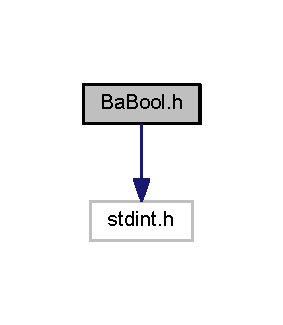
\includegraphics[width=136pt]{BaBool_8h__incl}
\end{center}
\end{figure}
This graph shows which files directly or indirectly include this file\+:\nopagebreak
\begin{figure}[H]
\begin{center}
\leavevmode
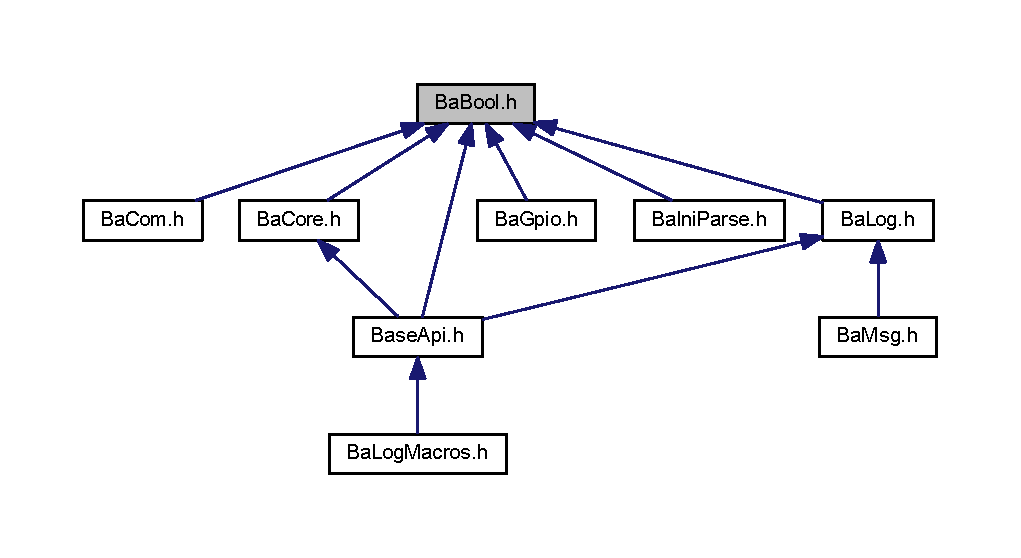
\includegraphics[width=350pt]{BaBool_8h__dep__incl}
\end{center}
\end{figure}
\subsection*{Typedefs}
\begin{DoxyCompactItemize}
\item 
\hypertarget{BaBool_8h_a5fe1eb8d6ba045ac2251a8f369c2e7b6}{}typedef int8\+\_\+t \hyperlink{BaBool_8h_a5fe1eb8d6ba045ac2251a8f369c2e7b6}{T\+Ba\+Bool}\label{BaBool_8h_a5fe1eb8d6ba045ac2251a8f369c2e7b6}

\begin{DoxyCompactList}\small\item\em General purpose pure C boolean type. \end{DoxyCompactList}\item 
\hypertarget{BaBool_8h_a84d5a0de4729ca4c89f2479c605dbf3d}{}typedef \hyperlink{BaBool_8h_a5fe1eb8d6ba045ac2251a8f369c2e7b6}{T\+Ba\+Bool} \hyperlink{BaBool_8h_a84d5a0de4729ca4c89f2479c605dbf3d}{T\+Ba\+Bool\+R\+C}\label{BaBool_8h_a84d5a0de4729ca4c89f2479c605dbf3d}

\begin{DoxyCompactList}\small\item\em General purpose pure C boolean return code type. \end{DoxyCompactList}\end{DoxyCompactItemize}


\subsection{Detailed Description}
General purpose pure C boolean type. 


\hypertarget{BaCom_8h}{}\section{Ba\+Com.\+h File Reference}
\label{BaCom_8h}\index{Ba\+Com.\+h@{Ba\+Com.\+h}}


Communications A\+P\+I.  


{\ttfamily \#include \char`\"{}Ba\+Bool.\+h\char`\"{}}\\*
Include dependency graph for Ba\+Com.\+h\+:\nopagebreak
\begin{figure}[H]
\begin{center}
\leavevmode
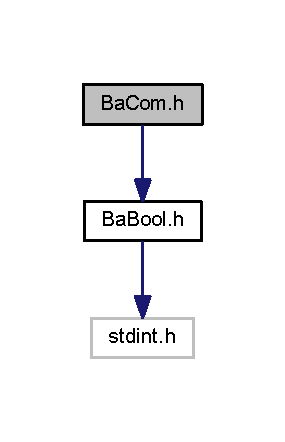
\includegraphics[width=137pt]{BaCom_8h__incl}
\end{center}
\end{figure}
\subsection*{Macros}
\begin{DoxyCompactItemize}
\item 
\hypertarget{BaCom_8h_a560d10625971945890a829c2cfd32769}{}\#define \hyperlink{BaCom_8h_a560d10625971945890a829c2cfd32769}{B\+A\+C\+O\+M\+\_\+\+S\+E\+R\+I\+A\+L\+D\+E\+V}~\char`\"{}/dev/tty\+A\+M\+A0\char`\"{}\label{BaCom_8h_a560d10625971945890a829c2cfd32769}

\begin{DoxyCompactList}\small\item\em Serial device path. \end{DoxyCompactList}\end{DoxyCompactItemize}
\subsection*{Typedefs}
\begin{DoxyCompactItemize}
\item 
\hypertarget{BaCom_8h_a0c2d065555852132f1e554bba19040db}{}typedef enum \hyperlink{BaCom_8h_a51ae55d0c5491b76a6070eb31390691d}{E\+Ba\+Com\+Baud} \hyperlink{BaCom_8h_a0c2d065555852132f1e554bba19040db}{E\+Ba\+Com\+Baud}\label{BaCom_8h_a0c2d065555852132f1e554bba19040db}

\begin{DoxyCompactList}\small\item\em Baud enumeration. \end{DoxyCompactList}\end{DoxyCompactItemize}
\subsection*{Enumerations}
\begin{DoxyCompactItemize}
\item 
\hypertarget{BaCom_8h_a51ae55d0c5491b76a6070eb31390691d}{}enum \hyperlink{BaCom_8h_a51ae55d0c5491b76a6070eb31390691d}{E\+Ba\+Com\+Baud} \label{BaCom_8h_a51ae55d0c5491b76a6070eb31390691d}
\begin{DoxyCompactList}\small\item\em Baud enumeration. \end{DoxyCompactList}
\end{DoxyCompactItemize}
\subsection*{Functions}
\begin{Indent}{\bf Init/\+Exit Functions}\par
\begin{DoxyCompactItemize}
\item 
T\+Ba\+Com\+Ser\+Hdl \hyperlink{BaCom_8h_afd029cee32185ec1613ba18b144439a2}{Ba\+Com\+Ser\+Init} (const char $\ast$device, \hyperlink{BaCom_8h_a51ae55d0c5491b76a6070eb31390691d}{E\+Ba\+Com\+Baud} baud)
\begin{DoxyCompactList}\small\item\em Initializes the resources and reserves G\+P\+I\+Os 14 and 15 for. \end{DoxyCompactList}\item 
\hyperlink{BaBool_8h_a84d5a0de4729ca4c89f2479c605dbf3d}{T\+Ba\+Bool\+R\+C} \hyperlink{BaCom_8h_a607a0ab43460b1e999519a8b6697e7f2}{Ba\+Com\+Ser\+Exit} (T\+Ba\+Com\+Ser\+Hdl hdl)
\begin{DoxyCompactList}\small\item\em Frees resources. \end{DoxyCompactList}\end{DoxyCompactItemize}
\end{Indent}


\subsection{Detailed Description}
Communications A\+P\+I. 


\begin{DoxyItemize}
\item I2\+C
\item S\+P\+I
\item Serial 
\end{DoxyItemize}

\subsection{Function Documentation}
\hypertarget{BaCom_8h_afd029cee32185ec1613ba18b144439a2}{}\index{Ba\+Com.\+h@{Ba\+Com.\+h}!Ba\+Com\+Ser\+Init@{Ba\+Com\+Ser\+Init}}
\index{Ba\+Com\+Ser\+Init@{Ba\+Com\+Ser\+Init}!Ba\+Com.\+h@{Ba\+Com.\+h}}
\subsubsection[{Ba\+Com\+Ser\+Init(const char $\ast$device, E\+Ba\+Com\+Baud baud)}]{\setlength{\rightskip}{0pt plus 5cm}T\+Ba\+Com\+Ser\+Hdl Ba\+Com\+Ser\+Init (
\begin{DoxyParamCaption}
\item[{const char $\ast$}]{device, }
\item[{{\bf E\+Ba\+Com\+Baud}}]{baud}
\end{DoxyParamCaption}
)}\label{BaCom_8h_afd029cee32185ec1613ba18b144439a2}


Initializes the resources and reserves G\+P\+I\+Os 14 and 15 for. 

\begin{DoxyReturn}{Returns}
Handle on success, otherwise error 
\end{DoxyReturn}

\begin{DoxyParams}{Parameters}
{\em device} & Device path, e.\+g. B\+A\+C\+O\+M\+\_\+\+S\+E\+R\+I\+A\+L\+D\+E\+V \\
\hline
{\em baud} & Baud rate \\
\hline
\end{DoxyParams}
\hypertarget{BaCom_8h_a607a0ab43460b1e999519a8b6697e7f2}{}\index{Ba\+Com.\+h@{Ba\+Com.\+h}!Ba\+Com\+Ser\+Exit@{Ba\+Com\+Ser\+Exit}}
\index{Ba\+Com\+Ser\+Exit@{Ba\+Com\+Ser\+Exit}!Ba\+Com.\+h@{Ba\+Com.\+h}}
\subsubsection[{Ba\+Com\+Ser\+Exit(\+T\+Ba\+Com\+Ser\+Hdl hdl)}]{\setlength{\rightskip}{0pt plus 5cm}{\bf T\+Ba\+Bool\+R\+C} Ba\+Com\+Ser\+Exit (
\begin{DoxyParamCaption}
\item[{T\+Ba\+Com\+Ser\+Hdl}]{hdl}
\end{DoxyParamCaption}
)}\label{BaCom_8h_a607a0ab43460b1e999519a8b6697e7f2}


Frees resources. 

\begin{DoxyReturn}{Returns}
Error or success 
\end{DoxyReturn}

\begin{DoxyParams}{Parameters}
{\em hdl} & Serial communication handle \\
\hline
\end{DoxyParams}

\hypertarget{BaCore_8h}{}\section{Ba\+Core.\+h File Reference}
\label{BaCore_8h}\index{Ba\+Core.\+h@{Ba\+Core.\+h}}


OS level A\+PI.  


{\ttfamily \#include $<$time.\+h$>$}\newline
{\ttfamily \#include \char`\"{}Ba\+Bool.\+h\char`\"{}}\newline
Include dependency graph for Ba\+Core.\+h\+:
\nopagebreak
\begin{figure}[H]
\begin{center}
\leavevmode
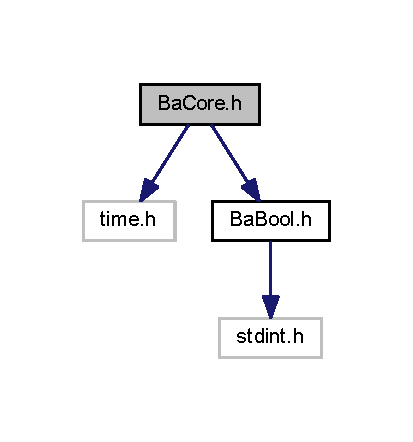
\includegraphics[width=198pt]{BaCore_8h__incl}
\end{center}
\end{figure}
This graph shows which files directly or indirectly include this file\+:
\nopagebreak
\begin{figure}[H]
\begin{center}
\leavevmode
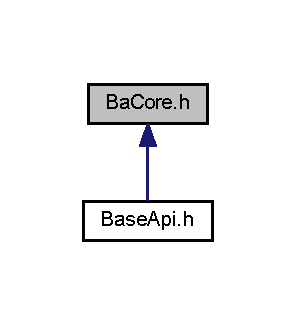
\includegraphics[width=308pt]{BaCore_8h__dep__incl}
\end{center}
\end{figure}
\subsection*{Classes}
\begin{DoxyCompactItemize}
\item 
struct \hyperlink{structTBaCoreTimeStamp}{T\+Ba\+Core\+Time\+Stamp}
\begin{DoxyCompactList}\small\item\em Time stamp structure. \end{DoxyCompactList}\item 
struct \hyperlink{structTBaCoreThreadArg}{T\+Ba\+Core\+Thread\+Arg}
\begin{DoxyCompactList}\small\item\em Thread function arguments. \end{DoxyCompactList}\item 
struct \hyperlink{structTBaCoreThreadInfo}{T\+Ba\+Core\+Thread\+Info}
\begin{DoxyCompactList}\small\item\em Thread info. \end{DoxyCompactList}\end{DoxyCompactItemize}
\subsection*{Typedefs}
\begin{DoxyCompactItemize}
\item 
\mbox{\Hypertarget{BaCore_8h_ab12ee629b9995a0696756e25fe0a85ef}\label{BaCore_8h_ab12ee629b9995a0696756e25fe0a85ef}} 
typedef struct \hyperlink{structTBaCoreTimeStamp}{T\+Ba\+Core\+Time\+Stamp} \hyperlink{BaCore_8h_ab12ee629b9995a0696756e25fe0a85ef}{T\+Ba\+Core\+Time\+Stamp}
\begin{DoxyCompactList}\small\item\em Time stamp structure. \end{DoxyCompactList}\item 
\mbox{\Hypertarget{BaCore_8h_a26e10ffbac03a898c7f8921f65ee4544}\label{BaCore_8h_a26e10ffbac03a898c7f8921f65ee4544}} 
typedef int64\+\_\+t \hyperlink{BaCore_8h_a26e10ffbac03a898c7f8921f65ee4544}{T\+Ba\+Core\+Mon\+T\+Stamp\+Us}
\begin{DoxyCompactList}\small\item\em Monotonic timestamp in microseconds. \end{DoxyCompactList}\item 
\mbox{\Hypertarget{BaCore_8h_a157dc8d9ee9a32912cbc26f9b1dd7476}\label{BaCore_8h_a157dc8d9ee9a32912cbc26f9b1dd7476}} 
typedef enum \hyperlink{BaCore_8h_a2021b3f630464ad65ce8f08ab10dc910}{E\+Ba\+Core\+Prio} \hyperlink{BaCore_8h_a157dc8d9ee9a32912cbc26f9b1dd7476}{E\+Ba\+Core\+Prio}
\begin{DoxyCompactList}\small\item\em Thread priority and scheduler. RT is F\+I\+FO. \end{DoxyCompactList}\item 
\mbox{\Hypertarget{BaCore_8h_a9a294779f7323469261016b0f040c297}\label{BaCore_8h_a9a294779f7323469261016b0f040c297}} 
typedef struct \hyperlink{structTBaCoreThreadArg}{T\+Ba\+Core\+Thread\+Arg} \hyperlink{BaCore_8h_a9a294779f7323469261016b0f040c297}{T\+Ba\+Core\+Thread\+Arg}
\begin{DoxyCompactList}\small\item\em Thread function arguments. \end{DoxyCompactList}\item 
\mbox{\Hypertarget{BaCore_8h_a55c2b904410b0e5f7b9b3f1b747a0475}\label{BaCore_8h_a55c2b904410b0e5f7b9b3f1b747a0475}} 
typedef struct \hyperlink{structTBaCoreThreadInfo}{T\+Ba\+Core\+Thread\+Info} \hyperlink{BaCore_8h_a55c2b904410b0e5f7b9b3f1b747a0475}{T\+Ba\+Core\+Thread\+Info}
\begin{DoxyCompactList}\small\item\em Thread info. \end{DoxyCompactList}\item 
\mbox{\Hypertarget{BaCore_8h_a41dc05559f1b0abe2f8261fc5cece7a9}\label{BaCore_8h_a41dc05559f1b0abe2f8261fc5cece7a9}} 
typedef void($\ast$ \hyperlink{BaCore_8h_a41dc05559f1b0abe2f8261fc5cece7a9}{T\+Ba\+Core\+Fun}) (void $\ast$arg)
\begin{DoxyCompactList}\small\item\em General function of the A\+PI. \end{DoxyCompactList}\item 
\mbox{\Hypertarget{BaCore_8h_ae50095c02ffddc39ec0df7f19e52c559}\label{BaCore_8h_ae50095c02ffddc39ec0df7f19e52c559}} 
typedef void($\ast$ \hyperlink{BaCore_8h_ae50095c02ffddc39ec0df7f19e52c559}{T\+Ba\+Core\+Thread\+Fun}) (\hyperlink{structTBaCoreThreadArg}{T\+Ba\+Core\+Thread\+Arg} $\ast$p\+Arg)
\begin{DoxyCompactList}\small\item\em Functions for threads. \end{DoxyCompactList}\item 
\mbox{\Hypertarget{BaCore_8h_a2898da7dd1b0e998b8c64dca81dff404}\label{BaCore_8h_a2898da7dd1b0e998b8c64dca81dff404}} 
typedef const void $\ast$ \hyperlink{BaCore_8h_a2898da7dd1b0e998b8c64dca81dff404}{T\+Ba\+Core\+Thread\+Hdl}
\begin{DoxyCompactList}\small\item\em Thread handle. \end{DoxyCompactList}\end{DoxyCompactItemize}
\subsection*{Enumerations}
\begin{DoxyCompactItemize}
\item 
enum \hyperlink{BaCore_8h_a2021b3f630464ad65ce8f08ab10dc910}{E\+Ba\+Core\+Prio} \{ \newline
\hyperlink{BaCore_8h_a2021b3f630464ad65ce8f08ab10dc910a5c9348f0471954d02479b1de2d0e0a5c}{e\+Ba\+Core\+Prio\+\_\+\+Minimum} = 0, 
\hyperlink{BaCore_8h_a2021b3f630464ad65ce8f08ab10dc910a18ae3d0630a0ecdc0202911cdb8bd0c8}{e\+Ba\+Core\+Prio\+\_\+\+Low}, 
\hyperlink{BaCore_8h_a2021b3f630464ad65ce8f08ab10dc910a64a4f256f9b0bae0d04f2fd20e6c4333}{e\+Ba\+Core\+Prio\+\_\+\+Normal}, 
\hyperlink{BaCore_8h_a2021b3f630464ad65ce8f08ab10dc910a232e29885fc570166ff832fde62ac33e}{e\+Ba\+Core\+Prio\+\_\+\+High}, 
\newline
\hyperlink{BaCore_8h_a2021b3f630464ad65ce8f08ab10dc910a109bf2120ebb826d6e87117e7a515bd5}{e\+Ba\+Core\+Prio\+\_\+\+Highest}, 
\hyperlink{BaCore_8h_a2021b3f630464ad65ce8f08ab10dc910aec172ae856b35d50314f66288709eabc}{e\+Ba\+Core\+Prio\+\_\+\+R\+T\+\_\+\+Normal}, 
\hyperlink{BaCore_8h_a2021b3f630464ad65ce8f08ab10dc910a22b7231add58f0a5ac53bcbc1bea9eca}{e\+Ba\+Core\+Prio\+\_\+\+R\+T\+\_\+\+High}, 
\hyperlink{BaCore_8h_a2021b3f630464ad65ce8f08ab10dc910a62b2c0516fe37f9cb7d91f45dbedecfd}{e\+Ba\+Core\+Prio\+\_\+\+R\+T\+\_\+\+Highest}
 \}\begin{DoxyCompactList}\small\item\em Thread priority and scheduler. RT is F\+I\+FO. \end{DoxyCompactList}
\end{DoxyCompactItemize}
\subsection*{Functions}
\begin{Indent}\textbf{ Sleep functions}\par
\begin{DoxyCompactItemize}
\item 
void \hyperlink{BaCore_8h_a6c94c2551e1b136347b5b67ff948fb8a}{Ba\+Core\+Sleep} (int64\+\_\+t s)
\begin{DoxyCompactList}\small\item\em Puts the thread to sleep and causes context change. \end{DoxyCompactList}\item 
void \hyperlink{BaCore_8h_a0b02663d5b06d203f8886a8b9702a055}{Ba\+Core\+M\+Sleep} (int64\+\_\+t ms)
\begin{DoxyCompactList}\small\item\em Puts the thread to sleep and causes context change. \end{DoxyCompactList}\item 
void \hyperlink{BaCore_8h_a1d944ec09e121ad1d73c342ef0040a7a}{Ba\+Core\+U\+Sleep} (int64\+\_\+t us)
\begin{DoxyCompactList}\small\item\em Puts the thread to sleep and causes context change. \end{DoxyCompactList}\item 
void \hyperlink{BaCore_8h_a3bdde8e7955f8575a7a7bf94609a8f0a}{Ba\+Core\+N\+Sleep} (int64\+\_\+t ns)
\begin{DoxyCompactList}\small\item\em Puts the thread to sleep and causes context change. \end{DoxyCompactList}\end{DoxyCompactItemize}
\end{Indent}
\begin{Indent}\textbf{ Timing functions}\par
\begin{DoxyCompactItemize}
\item 
int64\+\_\+t \hyperlink{BaCore_8h_a5753216c928d411b57f70254302157c9}{Ba\+Core\+TimedS} (\hyperlink{BaCore_8h_a41dc05559f1b0abe2f8261fc5cece7a9}{T\+Ba\+Core\+Fun} fun, void $\ast$p\+Arg)
\begin{DoxyCompactList}\small\item\em Timing function. \end{DoxyCompactList}\item 
int64\+\_\+t \hyperlink{BaCore_8h_a2ab9ab9bd8d9002a4bd017d4421e9260}{Ba\+Core\+Timed\+Ms} (\hyperlink{BaCore_8h_a41dc05559f1b0abe2f8261fc5cece7a9}{T\+Ba\+Core\+Fun} fun, void $\ast$p\+Arg)
\begin{DoxyCompactList}\small\item\em Timing function. \end{DoxyCompactList}\item 
int64\+\_\+t \hyperlink{BaCore_8h_ac7c70166fe4345034332c00a46d4946f}{Ba\+Core\+Timed\+Us} (\hyperlink{BaCore_8h_a41dc05559f1b0abe2f8261fc5cece7a9}{T\+Ba\+Core\+Fun} fun, void $\ast$p\+Arg)
\begin{DoxyCompactList}\small\item\em Timing function. \end{DoxyCompactList}\item 
void \hyperlink{BaCore_8h_a5890e7e91b8c1895f6a474781c489eb8}{Ba\+Core\+Get\+T\+Stamp} (\hyperlink{structTBaCoreTimeStamp}{T\+Ba\+Core\+Time\+Stamp} $\ast$p\+Stamp)
\begin{DoxyCompactList}\small\item\em Gets the actual timestamp in local timeS. \end{DoxyCompactList}\item 
\mbox{\Hypertarget{BaCore_8h_addc3e044eb80deaba6bcbf17e7549b7b}\label{BaCore_8h_addc3e044eb80deaba6bcbf17e7549b7b}} 
\hyperlink{BaCore_8h_a26e10ffbac03a898c7f8921f65ee4544}{T\+Ba\+Core\+Mon\+T\+Stamp\+Us} \hyperlink{BaCore_8h_addc3e044eb80deaba6bcbf17e7549b7b}{Ba\+Core\+Get\+Mon\+T\+Stamp} ()
\begin{DoxyCompactList}\small\item\em Gets the actual monotonic timestamp in microseconds. \end{DoxyCompactList}\item 
const char $\ast$ \hyperlink{BaCore_8h_a505f6901474517229290f1f9278f5a99}{Ba\+Core\+T\+Stamp\+To\+Str} (const \hyperlink{structTBaCoreTimeStamp}{T\+Ba\+Core\+Time\+Stamp} $\ast$p\+Stamp, char p\+Buf\mbox{[}B\+A\+C\+O\+R\+E\+\_\+\+T\+S\+T\+A\+M\+P\+L\+EN\mbox{]})
\begin{DoxyCompactList}\small\item\em Converts time stamp structure to string. \end{DoxyCompactList}\end{DoxyCompactItemize}
\end{Indent}
\begin{Indent}\textbf{ Multi-\/threading}\par
\begin{DoxyCompactItemize}
\item 
\hyperlink{BaCore_8h_a2898da7dd1b0e998b8c64dca81dff404}{T\+Ba\+Core\+Thread\+Hdl} \hyperlink{BaCore_8h_a91ad70ff751bb8afd38fe7fd3bc7e1e1}{Ba\+Core\+Create\+Thread} (const char $\ast$name, \hyperlink{BaCore_8h_ae50095c02ffddc39ec0df7f19e52c559}{T\+Ba\+Core\+Thread\+Fun} routine, \hyperlink{structTBaCoreThreadArg}{T\+Ba\+Core\+Thread\+Arg} $\ast$p\+Arg, \hyperlink{BaCore_8h_a2021b3f630464ad65ce8f08ab10dc910}{E\+Ba\+Core\+Prio} prio)
\begin{DoxyCompactList}\small\item\em Thread factory. \end{DoxyCompactList}\item 
\hyperlink{BaBool_8h_a84d5a0de4729ca4c89f2479c605dbf3d}{T\+Ba\+Bool\+RC} \hyperlink{BaCore_8h_a0135e688ca9ae4e687e4c774917e1067}{Ba\+Core\+Destroy\+Thread} (\hyperlink{BaCore_8h_a2898da7dd1b0e998b8c64dca81dff404}{T\+Ba\+Core\+Thread\+Hdl} hdl, uint32\+\_\+t timeout\+Ms)
\begin{DoxyCompactList}\small\item\em Thread destructor. \end{DoxyCompactList}\item 
\hyperlink{BaBool_8h_a84d5a0de4729ca4c89f2479c605dbf3d}{T\+Ba\+Bool\+RC} \hyperlink{BaCore_8h_a3063c6580150f08a015d37bcd9cd3bb6}{Ba\+Core\+Get\+Thread\+Info} (const \hyperlink{BaCore_8h_a2898da7dd1b0e998b8c64dca81dff404}{T\+Ba\+Core\+Thread\+Hdl} hdl, \hyperlink{structTBaCoreThreadInfo}{T\+Ba\+Core\+Thread\+Info} $\ast$p\+Info)
\begin{DoxyCompactList}\small\item\em Get the thread info. \end{DoxyCompactList}\end{DoxyCompactItemize}
\end{Indent}


\subsection{Detailed Description}
OS level A\+PI. 

Core functions include\+:
\begin{DoxyItemize}
\item Timers
\item Threads
\item Sleeps 
\end{DoxyItemize}

\subsection{Enumeration Type Documentation}
\mbox{\Hypertarget{BaCore_8h_a2021b3f630464ad65ce8f08ab10dc910}\label{BaCore_8h_a2021b3f630464ad65ce8f08ab10dc910}} 
\index{Ba\+Core.\+h@{Ba\+Core.\+h}!E\+Ba\+Core\+Prio@{E\+Ba\+Core\+Prio}}
\index{E\+Ba\+Core\+Prio@{E\+Ba\+Core\+Prio}!Ba\+Core.\+h@{Ba\+Core.\+h}}
\subsubsection{\texorpdfstring{E\+Ba\+Core\+Prio}{EBaCorePrio}}
{\footnotesize\ttfamily enum \hyperlink{BaCore_8h_a2021b3f630464ad65ce8f08ab10dc910}{E\+Ba\+Core\+Prio}}



Thread priority and scheduler. RT is F\+I\+FO. 

\begin{DoxyEnumFields}{Enumerator}
\raisebox{\heightof{T}}[0pt][0pt]{\index{e\+Ba\+Core\+Prio\+\_\+\+Minimum@{e\+Ba\+Core\+Prio\+\_\+\+Minimum}!Ba\+Core.\+h@{Ba\+Core.\+h}}\index{Ba\+Core.\+h@{Ba\+Core.\+h}!e\+Ba\+Core\+Prio\+\_\+\+Minimum@{e\+Ba\+Core\+Prio\+\_\+\+Minimum}}}\mbox{\Hypertarget{BaCore_8h_a2021b3f630464ad65ce8f08ab10dc910a5c9348f0471954d02479b1de2d0e0a5c}\label{BaCore_8h_a2021b3f630464ad65ce8f08ab10dc910a5c9348f0471954d02479b1de2d0e0a5c}} 
e\+Ba\+Core\+Prio\+\_\+\+Minimum&0 \\
\hline

\raisebox{\heightof{T}}[0pt][0pt]{\index{e\+Ba\+Core\+Prio\+\_\+\+Low@{e\+Ba\+Core\+Prio\+\_\+\+Low}!Ba\+Core.\+h@{Ba\+Core.\+h}}\index{Ba\+Core.\+h@{Ba\+Core.\+h}!e\+Ba\+Core\+Prio\+\_\+\+Low@{e\+Ba\+Core\+Prio\+\_\+\+Low}}}\mbox{\Hypertarget{BaCore_8h_a2021b3f630464ad65ce8f08ab10dc910a18ae3d0630a0ecdc0202911cdb8bd0c8}\label{BaCore_8h_a2021b3f630464ad65ce8f08ab10dc910a18ae3d0630a0ecdc0202911cdb8bd0c8}} 
e\+Ba\+Core\+Prio\+\_\+\+Low&1 \\
\hline

\raisebox{\heightof{T}}[0pt][0pt]{\index{e\+Ba\+Core\+Prio\+\_\+\+Normal@{e\+Ba\+Core\+Prio\+\_\+\+Normal}!Ba\+Core.\+h@{Ba\+Core.\+h}}\index{Ba\+Core.\+h@{Ba\+Core.\+h}!e\+Ba\+Core\+Prio\+\_\+\+Normal@{e\+Ba\+Core\+Prio\+\_\+\+Normal}}}\mbox{\Hypertarget{BaCore_8h_a2021b3f630464ad65ce8f08ab10dc910a64a4f256f9b0bae0d04f2fd20e6c4333}\label{BaCore_8h_a2021b3f630464ad65ce8f08ab10dc910a64a4f256f9b0bae0d04f2fd20e6c4333}} 
e\+Ba\+Core\+Prio\+\_\+\+Normal&2 \\
\hline

\raisebox{\heightof{T}}[0pt][0pt]{\index{e\+Ba\+Core\+Prio\+\_\+\+High@{e\+Ba\+Core\+Prio\+\_\+\+High}!Ba\+Core.\+h@{Ba\+Core.\+h}}\index{Ba\+Core.\+h@{Ba\+Core.\+h}!e\+Ba\+Core\+Prio\+\_\+\+High@{e\+Ba\+Core\+Prio\+\_\+\+High}}}\mbox{\Hypertarget{BaCore_8h_a2021b3f630464ad65ce8f08ab10dc910a232e29885fc570166ff832fde62ac33e}\label{BaCore_8h_a2021b3f630464ad65ce8f08ab10dc910a232e29885fc570166ff832fde62ac33e}} 
e\+Ba\+Core\+Prio\+\_\+\+High&3 \\
\hline

\raisebox{\heightof{T}}[0pt][0pt]{\index{e\+Ba\+Core\+Prio\+\_\+\+Highest@{e\+Ba\+Core\+Prio\+\_\+\+Highest}!Ba\+Core.\+h@{Ba\+Core.\+h}}\index{Ba\+Core.\+h@{Ba\+Core.\+h}!e\+Ba\+Core\+Prio\+\_\+\+Highest@{e\+Ba\+Core\+Prio\+\_\+\+Highest}}}\mbox{\Hypertarget{BaCore_8h_a2021b3f630464ad65ce8f08ab10dc910a109bf2120ebb826d6e87117e7a515bd5}\label{BaCore_8h_a2021b3f630464ad65ce8f08ab10dc910a109bf2120ebb826d6e87117e7a515bd5}} 
e\+Ba\+Core\+Prio\+\_\+\+Highest&4 \\
\hline

\raisebox{\heightof{T}}[0pt][0pt]{\index{e\+Ba\+Core\+Prio\+\_\+\+R\+T\+\_\+\+Normal@{e\+Ba\+Core\+Prio\+\_\+\+R\+T\+\_\+\+Normal}!Ba\+Core.\+h@{Ba\+Core.\+h}}\index{Ba\+Core.\+h@{Ba\+Core.\+h}!e\+Ba\+Core\+Prio\+\_\+\+R\+T\+\_\+\+Normal@{e\+Ba\+Core\+Prio\+\_\+\+R\+T\+\_\+\+Normal}}}\mbox{\Hypertarget{BaCore_8h_a2021b3f630464ad65ce8f08ab10dc910aec172ae856b35d50314f66288709eabc}\label{BaCore_8h_a2021b3f630464ad65ce8f08ab10dc910aec172ae856b35d50314f66288709eabc}} 
e\+Ba\+Core\+Prio\+\_\+\+R\+T\+\_\+\+Normal&5 \\
\hline

\raisebox{\heightof{T}}[0pt][0pt]{\index{e\+Ba\+Core\+Prio\+\_\+\+R\+T\+\_\+\+High@{e\+Ba\+Core\+Prio\+\_\+\+R\+T\+\_\+\+High}!Ba\+Core.\+h@{Ba\+Core.\+h}}\index{Ba\+Core.\+h@{Ba\+Core.\+h}!e\+Ba\+Core\+Prio\+\_\+\+R\+T\+\_\+\+High@{e\+Ba\+Core\+Prio\+\_\+\+R\+T\+\_\+\+High}}}\mbox{\Hypertarget{BaCore_8h_a2021b3f630464ad65ce8f08ab10dc910a22b7231add58f0a5ac53bcbc1bea9eca}\label{BaCore_8h_a2021b3f630464ad65ce8f08ab10dc910a22b7231add58f0a5ac53bcbc1bea9eca}} 
e\+Ba\+Core\+Prio\+\_\+\+R\+T\+\_\+\+High&6 \\
\hline

\raisebox{\heightof{T}}[0pt][0pt]{\index{e\+Ba\+Core\+Prio\+\_\+\+R\+T\+\_\+\+Highest@{e\+Ba\+Core\+Prio\+\_\+\+R\+T\+\_\+\+Highest}!Ba\+Core.\+h@{Ba\+Core.\+h}}\index{Ba\+Core.\+h@{Ba\+Core.\+h}!e\+Ba\+Core\+Prio\+\_\+\+R\+T\+\_\+\+Highest@{e\+Ba\+Core\+Prio\+\_\+\+R\+T\+\_\+\+Highest}}}\mbox{\Hypertarget{BaCore_8h_a2021b3f630464ad65ce8f08ab10dc910a62b2c0516fe37f9cb7d91f45dbedecfd}\label{BaCore_8h_a2021b3f630464ad65ce8f08ab10dc910a62b2c0516fe37f9cb7d91f45dbedecfd}} 
e\+Ba\+Core\+Prio\+\_\+\+R\+T\+\_\+\+Highest&7 \\
\hline

\end{DoxyEnumFields}


\subsection{Function Documentation}
\mbox{\Hypertarget{BaCore_8h_a6c94c2551e1b136347b5b67ff948fb8a}\label{BaCore_8h_a6c94c2551e1b136347b5b67ff948fb8a}} 
\index{Ba\+Core.\+h@{Ba\+Core.\+h}!Ba\+Core\+Sleep@{Ba\+Core\+Sleep}}
\index{Ba\+Core\+Sleep@{Ba\+Core\+Sleep}!Ba\+Core.\+h@{Ba\+Core.\+h}}
\subsubsection{\texorpdfstring{Ba\+Core\+Sleep()}{BaCoreSleep()}}
{\footnotesize\ttfamily void Ba\+Core\+Sleep (\begin{DoxyParamCaption}\item[{int64\+\_\+t}]{s }\end{DoxyParamCaption})}



Puts the thread to sleep and causes context change. 

if s = 0 $\vert$$\vert$ ms = 0 $\vert$$\vert$ us = 0, there is no sleep if ns = 0, the thread sleeps for one tick as specified by nanosleep() 
\begin{DoxyParams}[1]{Parameters}
\mbox{\tt in}  & {\em s} & Sleep time in s \\
\hline
\end{DoxyParams}
\mbox{\Hypertarget{BaCore_8h_a0b02663d5b06d203f8886a8b9702a055}\label{BaCore_8h_a0b02663d5b06d203f8886a8b9702a055}} 
\index{Ba\+Core.\+h@{Ba\+Core.\+h}!Ba\+Core\+M\+Sleep@{Ba\+Core\+M\+Sleep}}
\index{Ba\+Core\+M\+Sleep@{Ba\+Core\+M\+Sleep}!Ba\+Core.\+h@{Ba\+Core.\+h}}
\subsubsection{\texorpdfstring{Ba\+Core\+M\+Sleep()}{BaCoreMSleep()}}
{\footnotesize\ttfamily void Ba\+Core\+M\+Sleep (\begin{DoxyParamCaption}\item[{int64\+\_\+t}]{ms }\end{DoxyParamCaption})}



Puts the thread to sleep and causes context change. 

if s = 0 $\vert$$\vert$ ms = 0 $\vert$$\vert$ us = 0, there is no sleep if ns = 0, the thread sleeps for one tick as specified by nanosleep() 
\begin{DoxyParams}[1]{Parameters}
\mbox{\tt in}  & {\em ms} & Sleep time in ms \\
\hline
\end{DoxyParams}
\mbox{\Hypertarget{BaCore_8h_a1d944ec09e121ad1d73c342ef0040a7a}\label{BaCore_8h_a1d944ec09e121ad1d73c342ef0040a7a}} 
\index{Ba\+Core.\+h@{Ba\+Core.\+h}!Ba\+Core\+U\+Sleep@{Ba\+Core\+U\+Sleep}}
\index{Ba\+Core\+U\+Sleep@{Ba\+Core\+U\+Sleep}!Ba\+Core.\+h@{Ba\+Core.\+h}}
\subsubsection{\texorpdfstring{Ba\+Core\+U\+Sleep()}{BaCoreUSleep()}}
{\footnotesize\ttfamily void Ba\+Core\+U\+Sleep (\begin{DoxyParamCaption}\item[{int64\+\_\+t}]{us }\end{DoxyParamCaption})}



Puts the thread to sleep and causes context change. 

if s = 0 $\vert$$\vert$ ms = 0 $\vert$$\vert$ us = 0, there is no sleep if ns = 0, the thread sleeps for one tick as specified by nanosleep() 
\begin{DoxyParams}[1]{Parameters}
\mbox{\tt in}  & {\em us} & Sleep time in us \\
\hline
\end{DoxyParams}
\mbox{\Hypertarget{BaCore_8h_a3bdde8e7955f8575a7a7bf94609a8f0a}\label{BaCore_8h_a3bdde8e7955f8575a7a7bf94609a8f0a}} 
\index{Ba\+Core.\+h@{Ba\+Core.\+h}!Ba\+Core\+N\+Sleep@{Ba\+Core\+N\+Sleep}}
\index{Ba\+Core\+N\+Sleep@{Ba\+Core\+N\+Sleep}!Ba\+Core.\+h@{Ba\+Core.\+h}}
\subsubsection{\texorpdfstring{Ba\+Core\+N\+Sleep()}{BaCoreNSleep()}}
{\footnotesize\ttfamily void Ba\+Core\+N\+Sleep (\begin{DoxyParamCaption}\item[{int64\+\_\+t}]{ns }\end{DoxyParamCaption})}



Puts the thread to sleep and causes context change. 

if s = 0 $\vert$$\vert$ ms = 0 $\vert$$\vert$ us = 0, there is no sleep if ns = 0, the thread sleeps for one tick as specified by nanosleep() 
\begin{DoxyParams}[1]{Parameters}
\mbox{\tt in}  & {\em ns} & Sleep time in ns \\
\hline
\end{DoxyParams}
\mbox{\Hypertarget{BaCore_8h_a5753216c928d411b57f70254302157c9}\label{BaCore_8h_a5753216c928d411b57f70254302157c9}} 
\index{Ba\+Core.\+h@{Ba\+Core.\+h}!Ba\+Core\+TimedS@{Ba\+Core\+TimedS}}
\index{Ba\+Core\+TimedS@{Ba\+Core\+TimedS}!Ba\+Core.\+h@{Ba\+Core.\+h}}
\subsubsection{\texorpdfstring{Ba\+Core\+Timed\+S()}{BaCoreTimedS()}}
{\footnotesize\ttfamily int64\+\_\+t Ba\+Core\+TimedS (\begin{DoxyParamCaption}\item[{\hyperlink{BaCore_8h_a41dc05559f1b0abe2f8261fc5cece7a9}{T\+Ba\+Core\+Fun}}]{fun,  }\item[{void $\ast$}]{p\+Arg }\end{DoxyParamCaption})}



Timing function. 

\begin{DoxyReturn}{Returns}
Time in the defined unit 
\end{DoxyReturn}

\begin{DoxyParams}[1]{Parameters}
\mbox{\tt in}  & {\em fun} & Function to be timed \\
\hline
\mbox{\tt in}  & {\em p\+Arg} & Function arguments \\
\hline
\end{DoxyParams}
\mbox{\Hypertarget{BaCore_8h_a2ab9ab9bd8d9002a4bd017d4421e9260}\label{BaCore_8h_a2ab9ab9bd8d9002a4bd017d4421e9260}} 
\index{Ba\+Core.\+h@{Ba\+Core.\+h}!Ba\+Core\+Timed\+Ms@{Ba\+Core\+Timed\+Ms}}
\index{Ba\+Core\+Timed\+Ms@{Ba\+Core\+Timed\+Ms}!Ba\+Core.\+h@{Ba\+Core.\+h}}
\subsubsection{\texorpdfstring{Ba\+Core\+Timed\+Ms()}{BaCoreTimedMs()}}
{\footnotesize\ttfamily int64\+\_\+t Ba\+Core\+Timed\+Ms (\begin{DoxyParamCaption}\item[{\hyperlink{BaCore_8h_a41dc05559f1b0abe2f8261fc5cece7a9}{T\+Ba\+Core\+Fun}}]{fun,  }\item[{void $\ast$}]{p\+Arg }\end{DoxyParamCaption})}



Timing function. 

\begin{DoxyReturn}{Returns}
Time in the defined unit 
\end{DoxyReturn}

\begin{DoxyParams}[1]{Parameters}
\mbox{\tt in}  & {\em fun} & Function to be timed \\
\hline
\mbox{\tt in}  & {\em p\+Arg} & Function arguments \\
\hline
\end{DoxyParams}
\mbox{\Hypertarget{BaCore_8h_ac7c70166fe4345034332c00a46d4946f}\label{BaCore_8h_ac7c70166fe4345034332c00a46d4946f}} 
\index{Ba\+Core.\+h@{Ba\+Core.\+h}!Ba\+Core\+Timed\+Us@{Ba\+Core\+Timed\+Us}}
\index{Ba\+Core\+Timed\+Us@{Ba\+Core\+Timed\+Us}!Ba\+Core.\+h@{Ba\+Core.\+h}}
\subsubsection{\texorpdfstring{Ba\+Core\+Timed\+Us()}{BaCoreTimedUs()}}
{\footnotesize\ttfamily int64\+\_\+t Ba\+Core\+Timed\+Us (\begin{DoxyParamCaption}\item[{\hyperlink{BaCore_8h_a41dc05559f1b0abe2f8261fc5cece7a9}{T\+Ba\+Core\+Fun}}]{fun,  }\item[{void $\ast$}]{p\+Arg }\end{DoxyParamCaption})}



Timing function. 

\begin{DoxyReturn}{Returns}
Time in the defined unit 
\end{DoxyReturn}

\begin{DoxyParams}[1]{Parameters}
\mbox{\tt in}  & {\em fun} & Function to be timed \\
\hline
\mbox{\tt in}  & {\em p\+Arg} & Function arguments \\
\hline
\end{DoxyParams}
\mbox{\Hypertarget{BaCore_8h_a5890e7e91b8c1895f6a474781c489eb8}\label{BaCore_8h_a5890e7e91b8c1895f6a474781c489eb8}} 
\index{Ba\+Core.\+h@{Ba\+Core.\+h}!Ba\+Core\+Get\+T\+Stamp@{Ba\+Core\+Get\+T\+Stamp}}
\index{Ba\+Core\+Get\+T\+Stamp@{Ba\+Core\+Get\+T\+Stamp}!Ba\+Core.\+h@{Ba\+Core.\+h}}
\subsubsection{\texorpdfstring{Ba\+Core\+Get\+T\+Stamp()}{BaCoreGetTStamp()}}
{\footnotesize\ttfamily void Ba\+Core\+Get\+T\+Stamp (\begin{DoxyParamCaption}\item[{\hyperlink{structTBaCoreTimeStamp}{T\+Ba\+Core\+Time\+Stamp} $\ast$}]{p\+Stamp }\end{DoxyParamCaption})}



Gets the actual timestamp in local timeS. 


\begin{DoxyParams}[1]{Parameters}
\mbox{\tt out}  & {\em p\+Stamp} & Time stamp \\
\hline
\end{DoxyParams}
\mbox{\Hypertarget{BaCore_8h_a505f6901474517229290f1f9278f5a99}\label{BaCore_8h_a505f6901474517229290f1f9278f5a99}} 
\index{Ba\+Core.\+h@{Ba\+Core.\+h}!Ba\+Core\+T\+Stamp\+To\+Str@{Ba\+Core\+T\+Stamp\+To\+Str}}
\index{Ba\+Core\+T\+Stamp\+To\+Str@{Ba\+Core\+T\+Stamp\+To\+Str}!Ba\+Core.\+h@{Ba\+Core.\+h}}
\subsubsection{\texorpdfstring{Ba\+Core\+T\+Stamp\+To\+Str()}{BaCoreTStampToStr()}}
{\footnotesize\ttfamily const char$\ast$ Ba\+Core\+T\+Stamp\+To\+Str (\begin{DoxyParamCaption}\item[{const \hyperlink{structTBaCoreTimeStamp}{T\+Ba\+Core\+Time\+Stamp} $\ast$}]{p\+Stamp,  }\item[{char}]{p\+Buf\mbox{[}\+B\+A\+C\+O\+R\+E\+\_\+\+T\+S\+T\+A\+M\+P\+L\+E\+N\mbox{]} }\end{DoxyParamCaption})}



Converts time stamp structure to string. 

If the user gives a buffer ({\ttfamily p\+Buf}), it is used and returned. If the buffer is null, the string is mallocated and user must free the returned pointer to avoid memory leaks. The string is 22 char long and has the following format\+: Y/\+M/D h\+:min\+:s.\+ms \begin{DoxyReturn}{Returns}
Time stamp string if success, otherwise, null 
\end{DoxyReturn}

\begin{DoxyParams}[1]{Parameters}
\mbox{\tt in}  & {\em p\+Stamp} & Time stamp to convert to string \\
\hline
\mbox{\tt in,out}  & {\em p\+Buf} & Optional buffer of length $>$= B\+A\+C\+O\+R\+E\+\_\+\+T\+S\+T\+A\+M\+P\+L\+EN. If null, the string is mallocated $\ast$ \\
\hline
\end{DoxyParams}
\mbox{\Hypertarget{BaCore_8h_a91ad70ff751bb8afd38fe7fd3bc7e1e1}\label{BaCore_8h_a91ad70ff751bb8afd38fe7fd3bc7e1e1}} 
\index{Ba\+Core.\+h@{Ba\+Core.\+h}!Ba\+Core\+Create\+Thread@{Ba\+Core\+Create\+Thread}}
\index{Ba\+Core\+Create\+Thread@{Ba\+Core\+Create\+Thread}!Ba\+Core.\+h@{Ba\+Core.\+h}}
\subsubsection{\texorpdfstring{Ba\+Core\+Create\+Thread()}{BaCoreCreateThread()}}
{\footnotesize\ttfamily \hyperlink{BaCore_8h_a2898da7dd1b0e998b8c64dca81dff404}{T\+Ba\+Core\+Thread\+Hdl} Ba\+Core\+Create\+Thread (\begin{DoxyParamCaption}\item[{const char $\ast$}]{name,  }\item[{\hyperlink{BaCore_8h_ae50095c02ffddc39ec0df7f19e52c559}{T\+Ba\+Core\+Thread\+Fun}}]{routine,  }\item[{\hyperlink{structTBaCoreThreadArg}{T\+Ba\+Core\+Thread\+Arg} $\ast$}]{p\+Arg,  }\item[{\hyperlink{BaCore_8h_a2021b3f630464ad65ce8f08ab10dc910}{E\+Ba\+Core\+Prio}}]{prio }\end{DoxyParamCaption})}



Thread factory. 

The maximum {\ttfamily name} size including null is 16 \begin{DoxyReturn}{Returns}
Thread handle 
\end{DoxyReturn}

\begin{DoxyParams}[1]{Parameters}
\mbox{\tt in}  & {\em name} & Thread name. Max size is 15 chars + null \\
\hline
\mbox{\tt in}  & {\em routine} & Thread entry function \\
\hline
\mbox{\tt in}  & {\em p\+Arg} & Arguments of thread function \\
\hline
\mbox{\tt in}  & {\em prio} & Thread priority \\
\hline
\end{DoxyParams}
\mbox{\Hypertarget{BaCore_8h_a0135e688ca9ae4e687e4c774917e1067}\label{BaCore_8h_a0135e688ca9ae4e687e4c774917e1067}} 
\index{Ba\+Core.\+h@{Ba\+Core.\+h}!Ba\+Core\+Destroy\+Thread@{Ba\+Core\+Destroy\+Thread}}
\index{Ba\+Core\+Destroy\+Thread@{Ba\+Core\+Destroy\+Thread}!Ba\+Core.\+h@{Ba\+Core.\+h}}
\subsubsection{\texorpdfstring{Ba\+Core\+Destroy\+Thread()}{BaCoreDestroyThread()}}
{\footnotesize\ttfamily \hyperlink{BaBool_8h_a84d5a0de4729ca4c89f2479c605dbf3d}{T\+Ba\+Bool\+RC} Ba\+Core\+Destroy\+Thread (\begin{DoxyParamCaption}\item[{\hyperlink{BaCore_8h_a2898da7dd1b0e998b8c64dca81dff404}{T\+Ba\+Core\+Thread\+Hdl}}]{hdl,  }\item[{uint32\+\_\+t}]{timeout\+Ms }\end{DoxyParamCaption})}



Thread destructor. 

It signals the thread to end and waits a maximum of {\ttfamily time\+Out\+Ms} ms. If it timeouts, the thread detaches, stays alive, and releases the resources when the thread routine returns. \begin{DoxyReturn}{Returns}
Error if bad handle or timeout and {\ttfamily time\+Out\+Ms} != 0, otherwise, success 
\end{DoxyReturn}

\begin{DoxyParams}[1]{Parameters}
\mbox{\tt in}  & {\em hdl} & Thread handle \\
\hline
\mbox{\tt in}  & {\em timeout\+Ms} & Timeout to wait in ms. If zero, no timeout and behaves like an asynchronous call \\
\hline
\end{DoxyParams}
\mbox{\Hypertarget{BaCore_8h_a3063c6580150f08a015d37bcd9cd3bb6}\label{BaCore_8h_a3063c6580150f08a015d37bcd9cd3bb6}} 
\index{Ba\+Core.\+h@{Ba\+Core.\+h}!Ba\+Core\+Get\+Thread\+Info@{Ba\+Core\+Get\+Thread\+Info}}
\index{Ba\+Core\+Get\+Thread\+Info@{Ba\+Core\+Get\+Thread\+Info}!Ba\+Core.\+h@{Ba\+Core.\+h}}
\subsubsection{\texorpdfstring{Ba\+Core\+Get\+Thread\+Info()}{BaCoreGetThreadInfo()}}
{\footnotesize\ttfamily \hyperlink{BaBool_8h_a84d5a0de4729ca4c89f2479c605dbf3d}{T\+Ba\+Bool\+RC} Ba\+Core\+Get\+Thread\+Info (\begin{DoxyParamCaption}\item[{const \hyperlink{BaCore_8h_a2898da7dd1b0e998b8c64dca81dff404}{T\+Ba\+Core\+Thread\+Hdl}}]{hdl,  }\item[{\hyperlink{structTBaCoreThreadInfo}{T\+Ba\+Core\+Thread\+Info} $\ast$}]{p\+Info }\end{DoxyParamCaption})}



Get the thread info. 

\begin{DoxyReturn}{Returns}
Error or success 
\end{DoxyReturn}

\begin{DoxyParams}[1]{Parameters}
\mbox{\tt in}  & {\em hdl} & Thread handle \\
\hline
\mbox{\tt out}  & {\em p\+Info} & Thread info \\
\hline
\end{DoxyParams}

\hypertarget{BaGenMacros_8h}{}\section{Ba\+Gen\+Macros.\+h File Reference}
\label{BaGenMacros_8h}\index{Ba\+Gen\+Macros.\+h@{Ba\+Gen\+Macros.\+h}}


General Macros or generic templated functions.  


\subsection*{Macros}
\begin{DoxyCompactItemize}
\item 
\mbox{\Hypertarget{BaGenMacros_8h_a3758dd5d300a594312c95bc393378df0}\label{BaGenMacros_8h_a3758dd5d300a594312c95bc393378df0}} 
\#define \hyperlink{BaGenMacros_8h_a3758dd5d300a594312c95bc393378df0}{L\+O\+C\+AL}~static
\begin{DoxyCompactList}\small\item\em Used to signalize a local function in the implementation file of a C-\/\+A\+PI. \end{DoxyCompactList}\item 
\mbox{\Hypertarget{BaGenMacros_8h_acae8431a4d7babf7652e7d3734af0e62}\label{BaGenMacros_8h_acae8431a4d7babf7652e7d3734af0e62}} 
\#define \hyperlink{BaGenMacros_8h_acae8431a4d7babf7652e7d3734af0e62}{S\+I\+GN}(X,  Y)~(Y $<$ 0 ? (X $<$ 0 ? X \+: -\/X) \+: (X $<$ 0 ? -\/X \+: X))
\begin{DoxyCompactList}\small\item\em Returns a value with the same value as x and the same sign as y. \end{DoxyCompactList}\item 
\mbox{\Hypertarget{BaGenMacros_8h_a2eb03319e5ccdc1a14b73a7d8b1724de}\label{BaGenMacros_8h_a2eb03319e5ccdc1a14b73a7d8b1724de}} 
\#define \hyperlink{BaGenMacros_8h_a2eb03319e5ccdc1a14b73a7d8b1724de}{S\+QR}(X)~((X)$\ast$(X))
\begin{DoxyCompactList}\small\item\em Generic square function. \end{DoxyCompactList}\item 
\mbox{\Hypertarget{BaGenMacros_8h_a178d25c580b4df2644472311a0756d86}\label{BaGenMacros_8h_a178d25c580b4df2644472311a0756d86}} 
\#define \hyperlink{BaGenMacros_8h_a178d25c580b4df2644472311a0756d86}{S\+W\+A\+PT}(T,  X,  Y)~do \{T z; z = X; X=Y; Y=z;\} while (0)
\begin{DoxyCompactList}\small\item\em Swap for typed variables. \end{DoxyCompactList}\item 
\mbox{\Hypertarget{BaGenMacros_8h_a919dba5d5cb6ad3ce4df87973d24bcf0}\label{BaGenMacros_8h_a919dba5d5cb6ad3ce4df87973d24bcf0}} 
\#define \hyperlink{BaGenMacros_8h_a919dba5d5cb6ad3ce4df87973d24bcf0}{F\+L\+T\+\_\+\+EQ}(F\+L\+T1,  F\+L\+T2,  D\+E\+L\+TA)~(fabs((F\+L\+T1) -\/ (F\+L\+T2)) $<$ (D\+E\+L\+TA))
\begin{DoxyCompactList}\small\item\em Float equality with a delta. Requires math.\+h. \end{DoxyCompactList}\item 
\mbox{\Hypertarget{BaGenMacros_8h_aeccbc832685b82394b474605a03f9025}\label{BaGenMacros_8h_aeccbc832685b82394b474605a03f9025}} 
\#define \hyperlink{BaGenMacros_8h_aeccbc832685b82394b474605a03f9025}{R\+O\+U\+N\+D\+\_\+\+H\+A\+LF}(X)
\begin{DoxyCompactList}\small\item\em Roundto the nearest half. \end{DoxyCompactList}\item 
\mbox{\Hypertarget{BaGenMacros_8h_aa0746d479d8433b89404db6bd60f5449}\label{BaGenMacros_8h_aa0746d479d8433b89404db6bd60f5449}} 
\#define \hyperlink{BaGenMacros_8h_aa0746d479d8433b89404db6bd60f5449}{I\+N\+R\+A\+N\+GE}(V\+AL,  \hyperlink{BaGenMacros_8h_ad2f3678bf5eae3684fc497130b946eae}{M\+IN},  \hyperlink{BaGenMacros_8h_aff9931d7524c88e07743af6535b20761}{M\+AX})~((\hyperlink{BaGenMacros_8h_ad2f3678bf5eae3684fc497130b946eae}{M\+IN}) $<$= (V\+AL) \&\& (V\+AL) $<$= (\hyperlink{BaGenMacros_8h_aff9931d7524c88e07743af6535b20761}{M\+AX}))
\begin{DoxyCompactList}\small\item\em Returns if min $<$= val $<$= max. \end{DoxyCompactList}\item 
\mbox{\Hypertarget{BaGenMacros_8h_a65784f44e83fca19bb1dd56db5137cf2}\label{BaGenMacros_8h_a65784f44e83fca19bb1dd56db5137cf2}} 
\#define \hyperlink{BaGenMacros_8h_a65784f44e83fca19bb1dd56db5137cf2}{A\+R\+R\+A\+Y\+S\+I\+ZE}(A\+RR)~(sizeof(A\+RR) / sizeof(A\+RR\mbox{[}0\mbox{]}))
\begin{DoxyCompactList}\small\item\em Array size macro. \end{DoxyCompactList}\item 
\mbox{\Hypertarget{BaGenMacros_8h_ae302a31e4e1696bc276d54feb360607e}\label{BaGenMacros_8h_ae302a31e4e1696bc276d54feb360607e}} 
\#define \hyperlink{BaGenMacros_8h_ae302a31e4e1696bc276d54feb360607e}{S\+E\+T\+A\+RR}(A\+RR,  N,  V\+AL)
\begin{DoxyCompactList}\small\item\em Set all fields of an array A\+RR of size N to V\+AL. \end{DoxyCompactList}\item 
\mbox{\Hypertarget{BaGenMacros_8h_af61d20e17d227ebaa2bd697b92cf4a0e}\label{BaGenMacros_8h_af61d20e17d227ebaa2bd697b92cf4a0e}} 
\#define \hyperlink{BaGenMacros_8h_af61d20e17d227ebaa2bd697b92cf4a0e}{Z\+E\+R\+O\+A\+RR}(A\+RR,  N)~\hyperlink{BaGenMacros_8h_ae302a31e4e1696bc276d54feb360607e}{S\+E\+T\+A\+RR}(A\+RR, N, 0)
\begin{DoxyCompactList}\small\item\em Set all fields of an array A\+RR of size N to 0. \end{DoxyCompactList}\item 
\mbox{\Hypertarget{BaGenMacros_8h_a633384e5d5fa26e07db9e7d078b06117}\label{BaGenMacros_8h_a633384e5d5fa26e07db9e7d078b06117}} 
\#define \hyperlink{BaGenMacros_8h_a633384e5d5fa26e07db9e7d078b06117}{F\+I\+L\+E\+\_\+\+N\+A\+M\+E\+\_\+}~(strrchr(\+\_\+\+\_\+\+F\+I\+L\+E\+\_\+\+\_\+, \textquotesingle{}/\textquotesingle{}) ? strrchr(\+\_\+\+\_\+\+F\+I\+L\+E\+\_\+\+\_\+, \textquotesingle{}/\textquotesingle{}) + 1 \+: \+\_\+\+\_\+\+F\+I\+L\+E\+\_\+\+\_\+)
\begin{DoxyCompactList}\small\item\em Calculates the file name without the path. Eg\+: My\+File.\+cpp. Requires string.\+h. \end{DoxyCompactList}\item 
\#define \hyperlink{BaGenMacros_8h_a8170837187d85e164f0c7c58c7ce5e89}{T\+I\+M\+E\+\_\+\+F\+U\+N\+\_\+}(fun)
\begin{DoxyCompactList}\small\item\em Times a function or code part and prints the time in seconds to console. \end{DoxyCompactList}\end{DoxyCompactItemize}
\begin{Indent}\textbf{ Min and max limit macros}\par
\begin{DoxyCompactItemize}
\item 
\mbox{\Hypertarget{BaGenMacros_8h_ad2f3678bf5eae3684fc497130b946eae}\label{BaGenMacros_8h_ad2f3678bf5eae3684fc497130b946eae}} 
\#define \hyperlink{BaGenMacros_8h_ad2f3678bf5eae3684fc497130b946eae}{M\+IN}(X,  Y)~((X) $<$ (Y) ? (X) \+: (Y))
\begin{DoxyCompactList}\small\item\em Min and max macros for C primitive types. \end{DoxyCompactList}\item 
\mbox{\Hypertarget{BaGenMacros_8h_aff9931d7524c88e07743af6535b20761}\label{BaGenMacros_8h_aff9931d7524c88e07743af6535b20761}} 
\#define \hyperlink{BaGenMacros_8h_aff9931d7524c88e07743af6535b20761}{M\+AX}(X,  Y)~((X) $>$ (Y) ? (X) \+: (Y))
\begin{DoxyCompactList}\small\item\em Min and max macros for C primitive types. \end{DoxyCompactList}\item 
\mbox{\Hypertarget{BaGenMacros_8h_ac62c5416118ba1652760cd62f822465c}\label{BaGenMacros_8h_ac62c5416118ba1652760cd62f822465c}} 
\#define \hyperlink{BaGenMacros_8h_ac62c5416118ba1652760cd62f822465c}{M\+I\+N\+M\+AX}(V\+AR,  MI,  MA)~(\hyperlink{BaGenMacros_8h_ad2f3678bf5eae3684fc497130b946eae}{M\+IN}(\hyperlink{BaGenMacros_8h_aff9931d7524c88e07743af6535b20761}{M\+AX}(V\+AR, MI), MA))
\begin{DoxyCompactList}\small\item\em Min and max macros for C primitive types. \end{DoxyCompactList}\end{DoxyCompactItemize}
\end{Indent}
\subsection*{Functions}
\begin{DoxyCompactItemize}
\item 
\mbox{\Hypertarget{BaGenMacros_8h_af94e4e21ed04253852b7d127965b5801}\label{BaGenMacros_8h_af94e4e21ed04253852b7d127965b5801}} 
{\footnotesize template$<$class T $>$ }\\void \hyperlink{BaGenMacros_8h_af94e4e21ed04253852b7d127965b5801}{S\+W\+AP} (T \&x, T \&y)
\begin{DoxyCompactList}\small\item\em Generic swap function. \end{DoxyCompactList}\end{DoxyCompactItemize}


\subsection{Detailed Description}
General Macros or generic templated functions. 

Do not include this header in another header file, only in implementation files, .c or .cpp. 

\subsection{Macro Definition Documentation}
\mbox{\Hypertarget{BaGenMacros_8h_a8170837187d85e164f0c7c58c7ce5e89}\label{BaGenMacros_8h_a8170837187d85e164f0c7c58c7ce5e89}} 
\index{Ba\+Gen\+Macros.\+h@{Ba\+Gen\+Macros.\+h}!T\+I\+M\+E\+\_\+\+F\+U\+N\+\_\+@{T\+I\+M\+E\+\_\+\+F\+U\+N\+\_\+}}
\index{T\+I\+M\+E\+\_\+\+F\+U\+N\+\_\+@{T\+I\+M\+E\+\_\+\+F\+U\+N\+\_\+}!Ba\+Gen\+Macros.\+h@{Ba\+Gen\+Macros.\+h}}
\subsubsection{\texorpdfstring{T\+I\+M\+E\+\_\+\+F\+U\+N\+\_\+}{TIME\_FUN\_}}
{\footnotesize\ttfamily \#define T\+I\+M\+E\+\_\+\+F\+U\+N\+\_\+(\begin{DoxyParamCaption}\item[{}]{fun }\end{DoxyParamCaption})}

{\bfseries Value\+:}
\begin{DoxyCode}
\textcolor{keyword}{auto} start = std::chrono::steady\_clock::now(); \(\backslash\)
    fun; \(\backslash\)
    std::chrono::duration<double> dur = (std::chrono::steady\_clock::now() - start); \(\backslash\)
    std::cout << #fun << \textcolor{stringliteral}{": "} << dur.count() << \textcolor{stringliteral}{" s"} << std::endl;
\end{DoxyCode}


Times a function or code part and prints the time in seconds to console. 

Requires $<$chrono$>$ 
\hypertarget{BaGpio_8h}{}\section{Ba\+Gpio.\+h File Reference}
\label{BaGpio_8h}\index{Ba\+Gpio.\+h@{Ba\+Gpio.\+h}}


G\+P\+I\+Os A\+P\+Is.  


{\ttfamily \#include \char`\"{}Ba\+Bool.\+h\char`\"{}}\\*
Include dependency graph for Ba\+Gpio.\+h\+:
\nopagebreak
\begin{figure}[H]
\begin{center}
\leavevmode
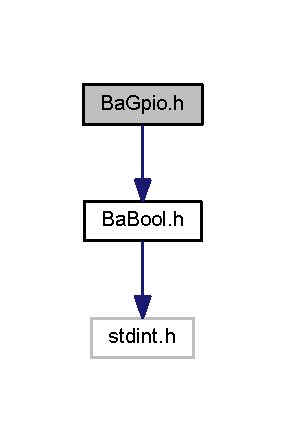
\includegraphics[width=137pt]{BaGpio_8h__incl}
\end{center}
\end{figure}
\subsection*{Classes}
\begin{DoxyCompactItemize}
\item 
class \hyperlink{classIBaGpio}{I\+Ba\+Gpio}
\begin{DoxyCompactList}\small\item\em C++ interface This is a C++ wrapper of the C A\+PI above adding multi process safety and a few extra functions. \end{DoxyCompactList}\end{DoxyCompactItemize}
\subsection*{Typedefs}
\begin{DoxyCompactItemize}
\item 
typedef uint8\+\_\+t \hyperlink{BaGpio_8h_aa287029c6ab2b66092b8e3b35ba41cb2}{T\+Ba\+Gpio}\hypertarget{BaGpio_8h_aa287029c6ab2b66092b8e3b35ba41cb2}{}\label{BaGpio_8h_aa287029c6ab2b66092b8e3b35ba41cb2}

\begin{DoxyCompactList}\small\item\em G\+P\+I\+Os range from 1 to 27. \end{DoxyCompactList}\item 
typedef void $\ast$ \hyperlink{BaGpio_8h_a0278073ad2b28a3a007b85f4b7e1cdb7}{T\+Ba\+Gpio\+S\+W\+P\+W\+M\+Hdl}\hypertarget{BaGpio_8h_a0278073ad2b28a3a007b85f4b7e1cdb7}{}\label{BaGpio_8h_a0278073ad2b28a3a007b85f4b7e1cdb7}

\begin{DoxyCompactList}\small\item\em Software P\+WM handle. \end{DoxyCompactList}\item 
typedef enum \hyperlink{BaGpio_8h_a63be35fa967e6932fc65444ce4a97f1f}{E\+Ba\+Gpio\+H\+W\+P\+W\+M\+Mode} \hyperlink{BaGpio_8h_abbc2af93a4290ff12e2e26ce87b86810}{E\+Ba\+Gpio\+H\+W\+P\+W\+M\+Mode}\hypertarget{BaGpio_8h_abbc2af93a4290ff12e2e26ce87b86810}{}\label{BaGpio_8h_abbc2af93a4290ff12e2e26ce87b86810}

\begin{DoxyCompactList}\small\item\em HW P\+WM mode flag. \end{DoxyCompactList}\end{DoxyCompactItemize}
\subsection*{Enumerations}
\subsection*{Functions}
\begin{Indent}{\bf Init/\+Exit Functions}\par
\begin{DoxyCompactItemize}
\item 
\hyperlink{BaBool_8h_a84d5a0de4729ca4c89f2479c605dbf3d}{T\+Ba\+Bool\+RC} \hyperlink{BaGpio_8h_ac45f705d6a118b9a6906eb4c2ead28e5}{Ba\+Gpio\+Init} ()
\begin{DoxyCompactList}\small\item\em Initializes and frees resources. \end{DoxyCompactList}\item 
\hyperlink{BaBool_8h_a84d5a0de4729ca4c89f2479c605dbf3d}{T\+Ba\+Bool\+RC} \hyperlink{BaGpio_8h_a4e73325028e7dc07512de8bc365f2aa5}{Ba\+Gpio\+Exit} ()
\begin{DoxyCompactList}\small\item\em Initializes and frees resources. \end{DoxyCompactList}\end{DoxyCompactItemize}
\end{Indent}
\begin{Indent}{\bf Hardware P\+WM setup functions}\par
\begin{DoxyCompactItemize}
\item 
\hyperlink{BaBool_8h_a84d5a0de4729ca4c89f2479c605dbf3d}{T\+Ba\+Bool\+RC} \hyperlink{BaGpio_8h_a7410dc8bd492a08566f8dce8f6d19409}{Ba\+Gpio\+Init\+H\+W\+P\+WM} ()
\begin{DoxyCompactList}\small\item\em Initialize the hardware P\+WM functionality with default frequency 1000 Hz and resolution 256 steps. \end{DoxyCompactList}\item 
\hyperlink{BaBool_8h_a84d5a0de4729ca4c89f2479c605dbf3d}{T\+Ba\+Bool\+RC} \hyperlink{BaGpio_8h_a03c0e46ed47943fea8e4693d0d779746}{Ba\+Gpio\+Exit\+H\+W\+P\+WM} ()
\begin{DoxyCompactList}\small\item\em Exit and release resources of the hardware P\+WM functionality. \end{DoxyCompactList}\item 
\hyperlink{BaBool_8h_a84d5a0de4729ca4c89f2479c605dbf3d}{T\+Ba\+Bool\+RC} \hyperlink{BaGpio_8h_a4212de0e0d110fc9c98bb0a03f91c720}{Ba\+Gpio\+Set\+Clk\+H\+W\+P\+WM} (double frequency, uint32\+\_\+t resolution, \hyperlink{BaGpio_8h_a63be35fa967e6932fc65444ce4a97f1f}{E\+Ba\+Gpio\+H\+W\+P\+W\+M\+Mode} mode)
\begin{DoxyCompactList}\small\item\em Set the frequency and resolution of the hardware P\+WM. \end{DoxyCompactList}\end{DoxyCompactItemize}
\end{Indent}
\begin{Indent}{\bf Basic G\+P\+IO operations}\par
\begin{DoxyCompactItemize}
\item 
\hyperlink{BaBool_8h_a84d5a0de4729ca4c89f2479c605dbf3d}{T\+Ba\+Bool\+RC} \hyperlink{BaGpio_8h_a1ff6ed95e15557ca3cc90f3339a94ccb}{Ba\+Gpio\+Clean\+Up} (\hyperlink{BaGpio_8h_aa287029c6ab2b66092b8e3b35ba41cb2}{T\+Ba\+Gpio} gpio)
\begin{DoxyCompactList}\small\item\em Cleans up the G\+P\+IO and leaves it on default state. \end{DoxyCompactList}\item 
\hyperlink{BaBool_8h_a84d5a0de4729ca4c89f2479c605dbf3d}{T\+Ba\+Bool\+RC} \hyperlink{BaGpio_8h_abbd38fa98845cf4593d50914e80163ec}{Ba\+Gpio\+Set\+Inp} (\hyperlink{BaGpio_8h_aa287029c6ab2b66092b8e3b35ba41cb2}{T\+Ba\+Gpio} gpio)
\begin{DoxyCompactList}\small\item\em Sets G\+P\+IO as input. \end{DoxyCompactList}\item 
\hyperlink{BaBool_8h_a84d5a0de4729ca4c89f2479c605dbf3d}{T\+Ba\+Bool\+RC} \hyperlink{BaGpio_8h_ade291c254be8b78a55e7e4cbd67dc280}{Ba\+Gpio\+Set\+Out} (\hyperlink{BaGpio_8h_aa287029c6ab2b66092b8e3b35ba41cb2}{T\+Ba\+Gpio} gpio)
\begin{DoxyCompactList}\small\item\em Sets G\+P\+IO as output. \end{DoxyCompactList}\item 
\hyperlink{BaBool_8h_a84d5a0de4729ca4c89f2479c605dbf3d}{T\+Ba\+Bool\+RC} \hyperlink{BaGpio_8h_a4e3556c9f680a78d0d64c055278e4757}{Ba\+Gpio\+Set\+Alt} (\hyperlink{BaGpio_8h_aa287029c6ab2b66092b8e3b35ba41cb2}{T\+Ba\+Gpio} gpio, int alt)
\begin{DoxyCompactList}\small\item\em Sets G\+P\+IO as alternative function. \end{DoxyCompactList}\item 
\hyperlink{BaBool_8h_a84d5a0de4729ca4c89f2479c605dbf3d}{T\+Ba\+Bool\+RC} \hyperlink{BaGpio_8h_a19bd984edf2725c2ba9143cd72a209ce}{Ba\+Gpio\+Set} (\hyperlink{BaGpio_8h_aa287029c6ab2b66092b8e3b35ba41cb2}{T\+Ba\+Gpio} gpio)
\begin{DoxyCompactList}\small\item\em Sets G\+P\+IO high. \end{DoxyCompactList}\item 
\hyperlink{BaBool_8h_a84d5a0de4729ca4c89f2479c605dbf3d}{T\+Ba\+Bool\+RC} \hyperlink{BaGpio_8h_a07a6c673d058de591cbbb1a204087b1c}{Ba\+Gpio\+Reset} (\hyperlink{BaGpio_8h_aa287029c6ab2b66092b8e3b35ba41cb2}{T\+Ba\+Gpio} gpio)
\begin{DoxyCompactList}\small\item\em Sets G\+P\+IO low. \end{DoxyCompactList}\item 
\hyperlink{BaBool_8h_a5fe1eb8d6ba045ac2251a8f369c2e7b6}{T\+Ba\+Bool} \hyperlink{BaGpio_8h_a33c51c0d60162284541644ab9b253728}{Ba\+Gpio\+Get} (\hyperlink{BaGpio_8h_aa287029c6ab2b66092b8e3b35ba41cb2}{T\+Ba\+Gpio} gpio)
\begin{DoxyCompactList}\small\item\em Gets the G\+P\+IO state high/low. \end{DoxyCompactList}\end{DoxyCompactItemize}
\end{Indent}
\begin{Indent}{\bf P\+WM Functions}\par
\begin{DoxyCompactItemize}
\item 
\hyperlink{BaBool_8h_a84d5a0de4729ca4c89f2479c605dbf3d}{T\+Ba\+Bool\+RC} \hyperlink{BaGpio_8h_a8cb36a42d8174d7feec21e7efe23a66e}{Ba\+Gpio\+Start\+H\+W\+P\+WM} (\hyperlink{BaGpio_8h_aa287029c6ab2b66092b8e3b35ba41cb2}{T\+Ba\+Gpio} gpio, float duty\+Cycle)
\begin{DoxyCompactList}\small\item\em Start the hardware P\+WM. \end{DoxyCompactList}\item 
\hyperlink{BaBool_8h_a84d5a0de4729ca4c89f2479c605dbf3d}{T\+Ba\+Bool\+RC} \hyperlink{BaGpio_8h_ac77888349ea2d6f446df57ee9805f859}{Ba\+Gpio\+Reset\+H\+W\+P\+W\+M\+Du\+Cy} (\hyperlink{BaGpio_8h_aa287029c6ab2b66092b8e3b35ba41cb2}{T\+Ba\+Gpio} gpio, float duty\+Cycle)
\begin{DoxyCompactList}\small\item\em Reset the duty cycle of the hardware P\+WM. \end{DoxyCompactList}\item 
\hyperlink{BaBool_8h_a84d5a0de4729ca4c89f2479c605dbf3d}{T\+Ba\+Bool\+RC} \hyperlink{BaGpio_8h_a03dc82924acee9df4ac55b298e549dfb}{Ba\+Gpio\+Stop\+H\+W\+P\+WM} (\hyperlink{BaGpio_8h_aa287029c6ab2b66092b8e3b35ba41cb2}{T\+Ba\+Gpio} gpio)
\begin{DoxyCompactList}\small\item\em Stop the hardware P\+WM. \end{DoxyCompactList}\item 
\hyperlink{BaGpio_8h_a0278073ad2b28a3a007b85f4b7e1cdb7}{T\+Ba\+Gpio\+S\+W\+P\+W\+M\+Hdl} \hyperlink{BaGpio_8h_aad89a86e462d6c700eb0f26a93d5c690}{Ba\+Gpio\+Start\+S\+W\+P\+WM} (\hyperlink{BaGpio_8h_aa287029c6ab2b66092b8e3b35ba41cb2}{T\+Ba\+Gpio} gpio, float dutyC, uint16\+\_\+t period\+Ms)
\begin{DoxyCompactList}\small\item\em Start software P\+WM on the desired G\+P\+IO with normal soft real-\/time priority. \end{DoxyCompactList}\item 
\hyperlink{BaBool_8h_a84d5a0de4729ca4c89f2479c605dbf3d}{T\+Ba\+Bool\+RC} \hyperlink{BaGpio_8h_ab2f6e0401076586a6f4b6d5fe7902b93}{Ba\+Gpio\+Reset\+S\+W\+P\+W\+M\+Du\+Cy} (\hyperlink{BaGpio_8h_a0278073ad2b28a3a007b85f4b7e1cdb7}{T\+Ba\+Gpio\+S\+W\+P\+W\+M\+Hdl} hdl, float dutyC)
\begin{DoxyCompactList}\small\item\em Reset the duty cycle of the software P\+WM. \end{DoxyCompactList}\item 
\hyperlink{BaBool_8h_a84d5a0de4729ca4c89f2479c605dbf3d}{T\+Ba\+Bool\+RC} \hyperlink{BaGpio_8h_a79b33d8a85223b99b6f6ad6d2fa6edc9}{Ba\+Gpio\+Stop\+S\+W\+P\+WM} (\hyperlink{BaGpio_8h_a0278073ad2b28a3a007b85f4b7e1cdb7}{T\+Ba\+Gpio\+S\+W\+P\+W\+M\+Hdl} hdl)
\begin{DoxyCompactList}\small\item\em Stop the software P\+WM. \end{DoxyCompactList}\end{DoxyCompactItemize}
\end{Indent}
\begin{Indent}{\bf C-\/\+Linkage object oriented factory}\par
\begin{DoxyCompactItemize}
\item 
\hyperlink{classIBaGpio}{I\+Ba\+Gpio} $\ast$ \hyperlink{BaGpio_8h_aebd32f84c3ed5166ee0f1bb99589b154}{I\+Ba\+Gpio\+Create} (\hyperlink{BaGpio_8h_aa287029c6ab2b66092b8e3b35ba41cb2}{T\+Ba\+Gpio} gpio)
\begin{DoxyCompactList}\small\item\em C++ interface object oriented factory. \end{DoxyCompactList}\item 
\hyperlink{BaBool_8h_a84d5a0de4729ca4c89f2479c605dbf3d}{T\+Ba\+Bool\+RC} \hyperlink{BaGpio_8h_a55b89951cd1565097e61c2f1eadfc948}{I\+Ba\+Gpio\+Delete} (\hyperlink{classIBaGpio}{I\+Ba\+Gpio} $\ast$p\+Hdl)
\begin{DoxyCompactList}\small\item\em C++ interface object oriented destructor. \end{DoxyCompactList}\end{DoxyCompactItemize}
\end{Indent}


\subsection{Detailed Description}
G\+P\+I\+Os A\+P\+Is. 

C A\+PI\+:~\newline

\begin{DoxyItemize}
\item The C A\+PI is thread-\/safe unless explicitly specified otherwise.
\item The C A\+PI has an initializations counter. Do not call the \hyperlink{BaGpio_8h_a4e73325028e7dc07512de8bc365f2aa5}{Ba\+Gpio\+Exit()} function without having called \hyperlink{BaGpio_8h_ac45f705d6a118b9a6906eb4c2ead28e5}{Ba\+Gpio\+Init()} first.
\item The C A\+PI is not multi-\/process safe. Processes can overwrite each other
\end{DoxyItemize}

C++ A\+PI~\newline
The object oriented C++ A\+PI is multiprocess safe between processes using this A\+PI 

\subsection{Enumeration Type Documentation}
\index{Ba\+Gpio.\+h@{Ba\+Gpio.\+h}!E\+Ba\+Gpio\+H\+W\+P\+W\+M\+Mode@{E\+Ba\+Gpio\+H\+W\+P\+W\+M\+Mode}}
\index{E\+Ba\+Gpio\+H\+W\+P\+W\+M\+Mode@{E\+Ba\+Gpio\+H\+W\+P\+W\+M\+Mode}!Ba\+Gpio.\+h@{Ba\+Gpio.\+h}}
\subsubsection[{\texorpdfstring{E\+Ba\+Gpio\+H\+W\+P\+W\+M\+Mode}{EBaGpioHWPWMMode}}]{\setlength{\rightskip}{0pt plus 5cm}enum {\bf E\+Ba\+Gpio\+H\+W\+P\+W\+M\+Mode}}\hypertarget{BaGpio_8h_a63be35fa967e6932fc65444ce4a97f1f}{}\label{BaGpio_8h_a63be35fa967e6932fc65444ce4a97f1f}


HW P\+WM mode flag. 

\begin{Desc}
\item[Enumerator]\par
\begin{description}
\index{E\+Ba\+Gpio\+H\+W\+P\+W\+M\+Mode\+\_\+\+Marked\+Space@{E\+Ba\+Gpio\+H\+W\+P\+W\+M\+Mode\+\_\+\+Marked\+Space}!Ba\+Gpio.\+h@{Ba\+Gpio.\+h}}\index{Ba\+Gpio.\+h@{Ba\+Gpio.\+h}!E\+Ba\+Gpio\+H\+W\+P\+W\+M\+Mode\+\_\+\+Marked\+Space@{E\+Ba\+Gpio\+H\+W\+P\+W\+M\+Mode\+\_\+\+Marked\+Space}}\item[{\em 
E\+Ba\+Gpio\+H\+W\+P\+W\+M\+Mode\+\_\+\+Marked\+Space\hypertarget{BaGpio_8h_a63be35fa967e6932fc65444ce4a97f1fa9adbab6b5a0d53ddf3fc7bf36763f404}{}\label{BaGpio_8h_a63be35fa967e6932fc65444ce4a97f1fa9adbab6b5a0d53ddf3fc7bf36763f404}
}]Traditional P\+WM mode. \index{E\+Ba\+Gpio\+H\+W\+P\+W\+M\+Mode\+\_\+\+Balanced@{E\+Ba\+Gpio\+H\+W\+P\+W\+M\+Mode\+\_\+\+Balanced}!Ba\+Gpio.\+h@{Ba\+Gpio.\+h}}\index{Ba\+Gpio.\+h@{Ba\+Gpio.\+h}!E\+Ba\+Gpio\+H\+W\+P\+W\+M\+Mode\+\_\+\+Balanced@{E\+Ba\+Gpio\+H\+W\+P\+W\+M\+Mode\+\_\+\+Balanced}}\item[{\em 
E\+Ba\+Gpio\+H\+W\+P\+W\+M\+Mode\+\_\+\+Balanced\hypertarget{BaGpio_8h_a63be35fa967e6932fc65444ce4a97f1fa5cb71a1a36c39d389b036c51dbbf3e36}{}\label{BaGpio_8h_a63be35fa967e6932fc65444ce4a97f1fa5cb71a1a36c39d389b036c51dbbf3e36}
}]Default mode. \end{description}
\end{Desc}


\subsection{Function Documentation}
\index{Ba\+Gpio.\+h@{Ba\+Gpio.\+h}!Ba\+Gpio\+Init@{Ba\+Gpio\+Init}}
\index{Ba\+Gpio\+Init@{Ba\+Gpio\+Init}!Ba\+Gpio.\+h@{Ba\+Gpio.\+h}}
\subsubsection[{\texorpdfstring{Ba\+Gpio\+Init()}{BaGpioInit()}}]{\setlength{\rightskip}{0pt plus 5cm}{\bf T\+Ba\+Bool\+RC} Ba\+Gpio\+Init (
\begin{DoxyParamCaption}
{}
\end{DoxyParamCaption}
)}\hypertarget{BaGpio_8h_ac45f705d6a118b9a6906eb4c2ead28e5}{}\label{BaGpio_8h_ac45f705d6a118b9a6906eb4c2ead28e5}


Initializes and frees resources. 

\begin{DoxyReturn}{Returns}
Error or success 
\end{DoxyReturn}


Referenced by Ba\+Gpio\+Stop\+S\+W\+P\+W\+M().

\index{Ba\+Gpio.\+h@{Ba\+Gpio.\+h}!Ba\+Gpio\+Exit@{Ba\+Gpio\+Exit}}
\index{Ba\+Gpio\+Exit@{Ba\+Gpio\+Exit}!Ba\+Gpio.\+h@{Ba\+Gpio.\+h}}
\subsubsection[{\texorpdfstring{Ba\+Gpio\+Exit()}{BaGpioExit()}}]{\setlength{\rightskip}{0pt plus 5cm}{\bf T\+Ba\+Bool\+RC} Ba\+Gpio\+Exit (
\begin{DoxyParamCaption}
{}
\end{DoxyParamCaption}
)}\hypertarget{BaGpio_8h_a4e73325028e7dc07512de8bc365f2aa5}{}\label{BaGpio_8h_a4e73325028e7dc07512de8bc365f2aa5}


Initializes and frees resources. 

\begin{DoxyReturn}{Returns}
Error or success 
\end{DoxyReturn}


Referenced by Ba\+Gpio\+Stop\+S\+W\+P\+W\+M().

\index{Ba\+Gpio.\+h@{Ba\+Gpio.\+h}!Ba\+Gpio\+Init\+H\+W\+P\+WM@{Ba\+Gpio\+Init\+H\+W\+P\+WM}}
\index{Ba\+Gpio\+Init\+H\+W\+P\+WM@{Ba\+Gpio\+Init\+H\+W\+P\+WM}!Ba\+Gpio.\+h@{Ba\+Gpio.\+h}}
\subsubsection[{\texorpdfstring{Ba\+Gpio\+Init\+H\+W\+P\+W\+M()}{BaGpioInitHWPWM()}}]{\setlength{\rightskip}{0pt plus 5cm}{\bf T\+Ba\+Bool\+RC} Ba\+Gpio\+Init\+H\+W\+P\+WM (
\begin{DoxyParamCaption}
{}
\end{DoxyParamCaption}
)}\hypertarget{BaGpio_8h_a7410dc8bd492a08566f8dce8f6d19409}{}\label{BaGpio_8h_a7410dc8bd492a08566f8dce8f6d19409}


Initialize the hardware P\+WM functionality with default frequency 1000 Hz and resolution 256 steps. 

W\+A\+R\+N\+I\+NG\+: The R\+PI uses the P\+WM subsystem to produce audio. As such please refrain from playing audio on the R\+PI while this code is running 

Referenced by Ba\+Gpio\+Stop\+S\+W\+P\+W\+M().

\index{Ba\+Gpio.\+h@{Ba\+Gpio.\+h}!Ba\+Gpio\+Exit\+H\+W\+P\+WM@{Ba\+Gpio\+Exit\+H\+W\+P\+WM}}
\index{Ba\+Gpio\+Exit\+H\+W\+P\+WM@{Ba\+Gpio\+Exit\+H\+W\+P\+WM}!Ba\+Gpio.\+h@{Ba\+Gpio.\+h}}
\subsubsection[{\texorpdfstring{Ba\+Gpio\+Exit\+H\+W\+P\+W\+M()}{BaGpioExitHWPWM()}}]{\setlength{\rightskip}{0pt plus 5cm}{\bf T\+Ba\+Bool\+RC} Ba\+Gpio\+Exit\+H\+W\+P\+WM (
\begin{DoxyParamCaption}
{}
\end{DoxyParamCaption}
)}\hypertarget{BaGpio_8h_a03c0e46ed47943fea8e4693d0d779746}{}\label{BaGpio_8h_a03c0e46ed47943fea8e4693d0d779746}


Exit and release resources of the hardware P\+WM functionality. 

\begin{DoxyReturn}{Returns}
Error or success 
\end{DoxyReturn}


Referenced by Ba\+Gpio\+Stop\+S\+W\+P\+W\+M().

\index{Ba\+Gpio.\+h@{Ba\+Gpio.\+h}!Ba\+Gpio\+Set\+Clk\+H\+W\+P\+WM@{Ba\+Gpio\+Set\+Clk\+H\+W\+P\+WM}}
\index{Ba\+Gpio\+Set\+Clk\+H\+W\+P\+WM@{Ba\+Gpio\+Set\+Clk\+H\+W\+P\+WM}!Ba\+Gpio.\+h@{Ba\+Gpio.\+h}}
\subsubsection[{\texorpdfstring{Ba\+Gpio\+Set\+Clk\+H\+W\+P\+W\+M(double frequency, uint32\+\_\+t resolution, E\+Ba\+Gpio\+H\+W\+P\+W\+M\+Mode mode)}{BaGpioSetClkHWPWM(double frequency, uint32_t resolution, EBaGpioHWPWMMode mode)}}]{\setlength{\rightskip}{0pt plus 5cm}{\bf T\+Ba\+Bool\+RC} Ba\+Gpio\+Set\+Clk\+H\+W\+P\+WM (
\begin{DoxyParamCaption}
\item[{double}]{frequency, }
\item[{uint32\+\_\+t}]{resolution, }
\item[{{\bf E\+Ba\+Gpio\+H\+W\+P\+W\+M\+Mode}}]{mode}
\end{DoxyParamCaption}
)}\hypertarget{BaGpio_8h_a4212de0e0d110fc9c98bb0a03f91c720}{}\label{BaGpio_8h_a4212de0e0d110fc9c98bb0a03f91c720}


Set the frequency and resolution of the hardware P\+WM. 

The clock frequency is 19.\+2 M\+Hz The maximum resolution is 4095 steps (12-\/bit) Please choose these wisely and bare in mind that the actual frequency is an estimate because only positive clock frequency divisors can be used. freq\+\_\+max @ min resolution (1-\/step) is 9.\+6 M\+Hz freq\+\_\+max @ max resolution (12-\/bit) is 2.\+34 k\+Hz Examples\+: freq\+\_\+max @ 1024-\/steps (10-\/bit) is 9.\+375 k\+Hz freq\+\_\+max @ 256-\/steps (8-\/bit) is 37.\+5 k\+Hz Conditions\+: frequency $\ast$ resolution $\ast$ 2 $<$ 19.\+2 M\+Hz resolution $<$= 4095 \begin{DoxyReturn}{Returns}
Error or success 
\end{DoxyReturn}

\begin{DoxyParams}[1]{Parameters}
\mbox{\tt in}  & {\em frequency} & desired frequency in Hz \\
\hline
\mbox{\tt in}  & {\em resolution} & desired resolution in steps \\
\hline
\mbox{\tt in}  & {\em mode} & P\+WM mode \\
\hline
\end{DoxyParams}


Referenced by Ba\+Gpio\+Init\+H\+W\+P\+W\+M(), and Ba\+Gpio\+Stop\+S\+W\+P\+W\+M().

\index{Ba\+Gpio.\+h@{Ba\+Gpio.\+h}!Ba\+Gpio\+Clean\+Up@{Ba\+Gpio\+Clean\+Up}}
\index{Ba\+Gpio\+Clean\+Up@{Ba\+Gpio\+Clean\+Up}!Ba\+Gpio.\+h@{Ba\+Gpio.\+h}}
\subsubsection[{\texorpdfstring{Ba\+Gpio\+Clean\+Up(\+T\+Ba\+Gpio gpio)}{BaGpioCleanUp(TBaGpio gpio)}}]{\setlength{\rightskip}{0pt plus 5cm}{\bf T\+Ba\+Bool\+RC} Ba\+Gpio\+Clean\+Up (
\begin{DoxyParamCaption}
\item[{{\bf T\+Ba\+Gpio}}]{gpio}
\end{DoxyParamCaption}
)}\hypertarget{BaGpio_8h_a1ff6ed95e15557ca3cc90f3339a94ccb}{}\label{BaGpio_8h_a1ff6ed95e15557ca3cc90f3339a94ccb}


Cleans up the G\+P\+IO and leaves it on default state. 

\begin{DoxyReturn}{Returns}
Error or success 
\end{DoxyReturn}

\begin{DoxyParams}[1]{Parameters}
\mbox{\tt in}  & {\em gpio} & G\+P\+IO number \\
\hline
\end{DoxyParams}


Referenced by Ba\+Gpio\+Stop\+S\+W\+P\+W\+M().

\index{Ba\+Gpio.\+h@{Ba\+Gpio.\+h}!Ba\+Gpio\+Set\+Inp@{Ba\+Gpio\+Set\+Inp}}
\index{Ba\+Gpio\+Set\+Inp@{Ba\+Gpio\+Set\+Inp}!Ba\+Gpio.\+h@{Ba\+Gpio.\+h}}
\subsubsection[{\texorpdfstring{Ba\+Gpio\+Set\+Inp(\+T\+Ba\+Gpio gpio)}{BaGpioSetInp(TBaGpio gpio)}}]{\setlength{\rightskip}{0pt plus 5cm}{\bf T\+Ba\+Bool\+RC} Ba\+Gpio\+Set\+Inp (
\begin{DoxyParamCaption}
\item[{{\bf T\+Ba\+Gpio}}]{gpio}
\end{DoxyParamCaption}
)}\hypertarget{BaGpio_8h_abbd38fa98845cf4593d50914e80163ec}{}\label{BaGpio_8h_abbd38fa98845cf4593d50914e80163ec}


Sets G\+P\+IO as input. 

\begin{DoxyReturn}{Returns}
Error or success 
\end{DoxyReturn}

\begin{DoxyParams}[1]{Parameters}
\mbox{\tt in}  & {\em gpio} & G\+P\+IO number \\
\hline
\end{DoxyParams}


Referenced by Ba\+Gpio\+Stop\+S\+W\+P\+W\+M().

\index{Ba\+Gpio.\+h@{Ba\+Gpio.\+h}!Ba\+Gpio\+Set\+Out@{Ba\+Gpio\+Set\+Out}}
\index{Ba\+Gpio\+Set\+Out@{Ba\+Gpio\+Set\+Out}!Ba\+Gpio.\+h@{Ba\+Gpio.\+h}}
\subsubsection[{\texorpdfstring{Ba\+Gpio\+Set\+Out(\+T\+Ba\+Gpio gpio)}{BaGpioSetOut(TBaGpio gpio)}}]{\setlength{\rightskip}{0pt plus 5cm}{\bf T\+Ba\+Bool\+RC} Ba\+Gpio\+Set\+Out (
\begin{DoxyParamCaption}
\item[{{\bf T\+Ba\+Gpio}}]{gpio}
\end{DoxyParamCaption}
)}\hypertarget{BaGpio_8h_ade291c254be8b78a55e7e4cbd67dc280}{}\label{BaGpio_8h_ade291c254be8b78a55e7e4cbd67dc280}


Sets G\+P\+IO as output. 

\begin{DoxyReturn}{Returns}
Error or success 
\end{DoxyReturn}

\begin{DoxyParams}[1]{Parameters}
\mbox{\tt in}  & {\em gpio} & G\+P\+IO number \\
\hline
\end{DoxyParams}


Referenced by Ba\+Gpio\+Start\+S\+W\+P\+W\+M(), and Ba\+Gpio\+Stop\+S\+W\+P\+W\+M().

\index{Ba\+Gpio.\+h@{Ba\+Gpio.\+h}!Ba\+Gpio\+Set\+Alt@{Ba\+Gpio\+Set\+Alt}}
\index{Ba\+Gpio\+Set\+Alt@{Ba\+Gpio\+Set\+Alt}!Ba\+Gpio.\+h@{Ba\+Gpio.\+h}}
\subsubsection[{\texorpdfstring{Ba\+Gpio\+Set\+Alt(\+T\+Ba\+Gpio gpio, int alt)}{BaGpioSetAlt(TBaGpio gpio, int alt)}}]{\setlength{\rightskip}{0pt plus 5cm}{\bf T\+Ba\+Bool\+RC} Ba\+Gpio\+Set\+Alt (
\begin{DoxyParamCaption}
\item[{{\bf T\+Ba\+Gpio}}]{gpio, }
\item[{int}]{alt}
\end{DoxyParamCaption}
)}\hypertarget{BaGpio_8h_a4e3556c9f680a78d0d64c055278e4757}{}\label{BaGpio_8h_a4e3556c9f680a78d0d64c055278e4757}


Sets G\+P\+IO as alternative function. 

\begin{DoxyReturn}{Returns}
Error or success 
\end{DoxyReturn}

\begin{DoxyParams}[1]{Parameters}
\mbox{\tt in}  & {\em gpio} & G\+P\+IO number \\
\hline
\mbox{\tt in}  & {\em alt} & Alternative function of G\+P\+IO \\
\hline
\end{DoxyParams}


Referenced by Ba\+Gpio\+Stop\+S\+W\+P\+W\+M().

\index{Ba\+Gpio.\+h@{Ba\+Gpio.\+h}!Ba\+Gpio\+Set@{Ba\+Gpio\+Set}}
\index{Ba\+Gpio\+Set@{Ba\+Gpio\+Set}!Ba\+Gpio.\+h@{Ba\+Gpio.\+h}}
\subsubsection[{\texorpdfstring{Ba\+Gpio\+Set(\+T\+Ba\+Gpio gpio)}{BaGpioSet(TBaGpio gpio)}}]{\setlength{\rightskip}{0pt plus 5cm}{\bf T\+Ba\+Bool\+RC} Ba\+Gpio\+Set (
\begin{DoxyParamCaption}
\item[{{\bf T\+Ba\+Gpio}}]{gpio}
\end{DoxyParamCaption}
)}\hypertarget{BaGpio_8h_a19bd984edf2725c2ba9143cd72a209ce}{}\label{BaGpio_8h_a19bd984edf2725c2ba9143cd72a209ce}


Sets G\+P\+IO high. 

Not thread safe for performance reasons \begin{DoxyReturn}{Returns}
Error or success 
\end{DoxyReturn}

\begin{DoxyParams}[1]{Parameters}
\mbox{\tt in}  & {\em gpio} & G\+P\+IO number \\
\hline
\end{DoxyParams}


Referenced by Ba\+Gpio\+Stop\+S\+W\+P\+W\+M().

\index{Ba\+Gpio.\+h@{Ba\+Gpio.\+h}!Ba\+Gpio\+Reset@{Ba\+Gpio\+Reset}}
\index{Ba\+Gpio\+Reset@{Ba\+Gpio\+Reset}!Ba\+Gpio.\+h@{Ba\+Gpio.\+h}}
\subsubsection[{\texorpdfstring{Ba\+Gpio\+Reset(\+T\+Ba\+Gpio gpio)}{BaGpioReset(TBaGpio gpio)}}]{\setlength{\rightskip}{0pt plus 5cm}{\bf T\+Ba\+Bool\+RC} Ba\+Gpio\+Reset (
\begin{DoxyParamCaption}
\item[{{\bf T\+Ba\+Gpio}}]{gpio}
\end{DoxyParamCaption}
)}\hypertarget{BaGpio_8h_a07a6c673d058de591cbbb1a204087b1c}{}\label{BaGpio_8h_a07a6c673d058de591cbbb1a204087b1c}


Sets G\+P\+IO low. 

Not thread safe for performance reasons \begin{DoxyReturn}{Returns}
Error or success 
\end{DoxyReturn}

\begin{DoxyParams}[1]{Parameters}
\mbox{\tt in}  & {\em gpio} & G\+P\+IO number \\
\hline
\end{DoxyParams}


Referenced by Ba\+Gpio\+Stop\+S\+W\+P\+W\+M().

\index{Ba\+Gpio.\+h@{Ba\+Gpio.\+h}!Ba\+Gpio\+Get@{Ba\+Gpio\+Get}}
\index{Ba\+Gpio\+Get@{Ba\+Gpio\+Get}!Ba\+Gpio.\+h@{Ba\+Gpio.\+h}}
\subsubsection[{\texorpdfstring{Ba\+Gpio\+Get(\+T\+Ba\+Gpio gpio)}{BaGpioGet(TBaGpio gpio)}}]{\setlength{\rightskip}{0pt plus 5cm}{\bf T\+Ba\+Bool} Ba\+Gpio\+Get (
\begin{DoxyParamCaption}
\item[{{\bf T\+Ba\+Gpio}}]{gpio}
\end{DoxyParamCaption}
)}\hypertarget{BaGpio_8h_a33c51c0d60162284541644ab9b253728}{}\label{BaGpio_8h_a33c51c0d60162284541644ab9b253728}


Gets the G\+P\+IO state high/low. 

\begin{DoxyReturn}{Returns}
high true, or low false 
\end{DoxyReturn}

\begin{DoxyParams}[1]{Parameters}
\mbox{\tt in}  & {\em gpio} & G\+P\+IO number \\
\hline
\end{DoxyParams}


Referenced by Ba\+Gpio\+Stop\+S\+W\+P\+W\+M().

\index{Ba\+Gpio.\+h@{Ba\+Gpio.\+h}!Ba\+Gpio\+Start\+H\+W\+P\+WM@{Ba\+Gpio\+Start\+H\+W\+P\+WM}}
\index{Ba\+Gpio\+Start\+H\+W\+P\+WM@{Ba\+Gpio\+Start\+H\+W\+P\+WM}!Ba\+Gpio.\+h@{Ba\+Gpio.\+h}}
\subsubsection[{\texorpdfstring{Ba\+Gpio\+Start\+H\+W\+P\+W\+M(\+T\+Ba\+Gpio gpio, float duty\+Cycle)}{BaGpioStartHWPWM(TBaGpio gpio, float dutyCycle)}}]{\setlength{\rightskip}{0pt plus 5cm}{\bf T\+Ba\+Bool\+RC} Ba\+Gpio\+Start\+H\+W\+P\+WM (
\begin{DoxyParamCaption}
\item[{{\bf T\+Ba\+Gpio}}]{gpio, }
\item[{float}]{duty\+Cycle}
\end{DoxyParamCaption}
)}\hypertarget{BaGpio_8h_a8cb36a42d8174d7feec21e7efe23a66e}{}\label{BaGpio_8h_a8cb36a42d8174d7feec21e7efe23a66e}


Start the hardware P\+WM. 

The \hyperlink{BaGpio_8h_a7410dc8bd492a08566f8dce8f6d19409}{Ba\+Gpio\+Init\+H\+W\+P\+W\+M()} function must be called before starting the HW P\+WM. Only G\+P\+I\+Os 12, 13, 18, and 19 can be rerouted to the P\+WM. \begin{DoxyReturn}{Returns}
Error or success 
\end{DoxyReturn}

\begin{DoxyParams}[1]{Parameters}
\mbox{\tt in}  & {\em gpio} & G\+P\+IO number \\
\hline
\mbox{\tt in}  & {\em duty\+Cycle} & Desired duty cycle \mbox{[}0..1\mbox{]} \\
\hline
\end{DoxyParams}


Referenced by Ba\+Gpio\+Stop\+S\+W\+P\+W\+M().

\index{Ba\+Gpio.\+h@{Ba\+Gpio.\+h}!Ba\+Gpio\+Reset\+H\+W\+P\+W\+M\+Du\+Cy@{Ba\+Gpio\+Reset\+H\+W\+P\+W\+M\+Du\+Cy}}
\index{Ba\+Gpio\+Reset\+H\+W\+P\+W\+M\+Du\+Cy@{Ba\+Gpio\+Reset\+H\+W\+P\+W\+M\+Du\+Cy}!Ba\+Gpio.\+h@{Ba\+Gpio.\+h}}
\subsubsection[{\texorpdfstring{Ba\+Gpio\+Reset\+H\+W\+P\+W\+M\+Du\+Cy(\+T\+Ba\+Gpio gpio, float duty\+Cycle)}{BaGpioResetHWPWMDuCy(TBaGpio gpio, float dutyCycle)}}]{\setlength{\rightskip}{0pt plus 5cm}{\bf T\+Ba\+Bool\+RC} Ba\+Gpio\+Reset\+H\+W\+P\+W\+M\+Du\+Cy (
\begin{DoxyParamCaption}
\item[{{\bf T\+Ba\+Gpio}}]{gpio, }
\item[{float}]{duty\+Cycle}
\end{DoxyParamCaption}
)}\hypertarget{BaGpio_8h_ac77888349ea2d6f446df57ee9805f859}{}\label{BaGpio_8h_ac77888349ea2d6f446df57ee9805f859}


Reset the duty cycle of the hardware P\+WM. 

\hyperlink{BaGpio_8h_a8cb36a42d8174d7feec21e7efe23a66e}{Ba\+Gpio\+Start\+H\+W\+P\+W\+M()} must be called before reseting the duty cycle. Not thread safe for performance reasons. \begin{DoxyReturn}{Returns}
Error or success 
\end{DoxyReturn}

\begin{DoxyParams}[1]{Parameters}
\mbox{\tt in}  & {\em gpio} & G\+P\+IO number \\
\hline
\mbox{\tt in}  & {\em duty\+Cycle} & Desired duty cycle \mbox{[}0..1\mbox{]} \\
\hline
\end{DoxyParams}


Referenced by Ba\+Gpio\+Stop\+S\+W\+P\+W\+M().

\index{Ba\+Gpio.\+h@{Ba\+Gpio.\+h}!Ba\+Gpio\+Stop\+H\+W\+P\+WM@{Ba\+Gpio\+Stop\+H\+W\+P\+WM}}
\index{Ba\+Gpio\+Stop\+H\+W\+P\+WM@{Ba\+Gpio\+Stop\+H\+W\+P\+WM}!Ba\+Gpio.\+h@{Ba\+Gpio.\+h}}
\subsubsection[{\texorpdfstring{Ba\+Gpio\+Stop\+H\+W\+P\+W\+M(\+T\+Ba\+Gpio gpio)}{BaGpioStopHWPWM(TBaGpio gpio)}}]{\setlength{\rightskip}{0pt plus 5cm}{\bf T\+Ba\+Bool\+RC} Ba\+Gpio\+Stop\+H\+W\+P\+WM (
\begin{DoxyParamCaption}
\item[{{\bf T\+Ba\+Gpio}}]{gpio}
\end{DoxyParamCaption}
)}\hypertarget{BaGpio_8h_a03dc82924acee9df4ac55b298e549dfb}{}\label{BaGpio_8h_a03dc82924acee9df4ac55b298e549dfb}


Stop the hardware P\+WM. 

\begin{DoxyReturn}{Returns}
Error or success 
\end{DoxyReturn}

\begin{DoxyParams}[1]{Parameters}
\mbox{\tt in}  & {\em gpio} & G\+P\+IO number \\
\hline
\end{DoxyParams}


Referenced by Ba\+Gpio\+Stop\+S\+W\+P\+W\+M().

\index{Ba\+Gpio.\+h@{Ba\+Gpio.\+h}!Ba\+Gpio\+Start\+S\+W\+P\+WM@{Ba\+Gpio\+Start\+S\+W\+P\+WM}}
\index{Ba\+Gpio\+Start\+S\+W\+P\+WM@{Ba\+Gpio\+Start\+S\+W\+P\+WM}!Ba\+Gpio.\+h@{Ba\+Gpio.\+h}}
\subsubsection[{\texorpdfstring{Ba\+Gpio\+Start\+S\+W\+P\+W\+M(\+T\+Ba\+Gpio gpio, float duty\+C, uint16\+\_\+t period\+Ms)}{BaGpioStartSWPWM(TBaGpio gpio, float dutyC, uint16_t periodMs)}}]{\setlength{\rightskip}{0pt plus 5cm}{\bf T\+Ba\+Gpio\+S\+W\+P\+W\+M\+Hdl} Ba\+Gpio\+Start\+S\+W\+P\+WM (
\begin{DoxyParamCaption}
\item[{{\bf T\+Ba\+Gpio}}]{gpio, }
\item[{float}]{dutyC, }
\item[{uint16\+\_\+t}]{period\+Ms}
\end{DoxyParamCaption}
)}\hypertarget{BaGpio_8h_aad89a86e462d6c700eb0f26a93d5c690}{}\label{BaGpio_8h_aad89a86e462d6c700eb0f26a93d5c690}


Start software P\+WM on the desired G\+P\+IO with normal soft real-\/time priority. 

The period must between 10 and 10000 ms. Input outside range will be limited. The faster the period, the more C\+PU usage. \begin{DoxyReturn}{Returns}
The software P\+WM handle if success, otherwise, null 
\end{DoxyReturn}

\begin{DoxyParams}[1]{Parameters}
\mbox{\tt in}  & {\em gpio} & Desired G\+P\+IO \\
\hline
\mbox{\tt in}  & {\em dutyC} & Initial duty cycle \mbox{[}0..1\mbox{]} \\
\hline
\mbox{\tt in}  & {\em period\+Ms} & P\+WM period in ms \mbox{[}10..10000\mbox{]} \\
\hline
\end{DoxyParams}


Referenced by Ba\+Gpio\+Stop\+S\+W\+P\+W\+M().

\index{Ba\+Gpio.\+h@{Ba\+Gpio.\+h}!Ba\+Gpio\+Reset\+S\+W\+P\+W\+M\+Du\+Cy@{Ba\+Gpio\+Reset\+S\+W\+P\+W\+M\+Du\+Cy}}
\index{Ba\+Gpio\+Reset\+S\+W\+P\+W\+M\+Du\+Cy@{Ba\+Gpio\+Reset\+S\+W\+P\+W\+M\+Du\+Cy}!Ba\+Gpio.\+h@{Ba\+Gpio.\+h}}
\subsubsection[{\texorpdfstring{Ba\+Gpio\+Reset\+S\+W\+P\+W\+M\+Du\+Cy(\+T\+Ba\+Gpio\+S\+W\+P\+W\+M\+Hdl hdl, float duty\+C)}{BaGpioResetSWPWMDuCy(TBaGpioSWPWMHdl hdl, float dutyC)}}]{\setlength{\rightskip}{0pt plus 5cm}{\bf T\+Ba\+Bool\+RC} Ba\+Gpio\+Reset\+S\+W\+P\+W\+M\+Du\+Cy (
\begin{DoxyParamCaption}
\item[{{\bf T\+Ba\+Gpio\+S\+W\+P\+W\+M\+Hdl}}]{hdl, }
\item[{float}]{dutyC}
\end{DoxyParamCaption}
)}\hypertarget{BaGpio_8h_ab2f6e0401076586a6f4b6d5fe7902b93}{}\label{BaGpio_8h_ab2f6e0401076586a6f4b6d5fe7902b93}


Reset the duty cycle of the software P\+WM. 

\begin{DoxyReturn}{Returns}
Error or success 
\end{DoxyReturn}

\begin{DoxyParams}[1]{Parameters}
\mbox{\tt in}  & {\em hdl} & Software P\+WM handle \\
\hline
\mbox{\tt in}  & {\em dutyC} & Desired duty cycle \mbox{[}0..1\mbox{]} \\
\hline
\end{DoxyParams}


Referenced by Ba\+Gpio\+Stop\+S\+W\+P\+W\+M().

\index{Ba\+Gpio.\+h@{Ba\+Gpio.\+h}!Ba\+Gpio\+Stop\+S\+W\+P\+WM@{Ba\+Gpio\+Stop\+S\+W\+P\+WM}}
\index{Ba\+Gpio\+Stop\+S\+W\+P\+WM@{Ba\+Gpio\+Stop\+S\+W\+P\+WM}!Ba\+Gpio.\+h@{Ba\+Gpio.\+h}}
\subsubsection[{\texorpdfstring{Ba\+Gpio\+Stop\+S\+W\+P\+W\+M(\+T\+Ba\+Gpio\+S\+W\+P\+W\+M\+Hdl hdl)}{BaGpioStopSWPWM(TBaGpioSWPWMHdl hdl)}}]{\setlength{\rightskip}{0pt plus 5cm}{\bf T\+Ba\+Bool\+RC} Ba\+Gpio\+Stop\+S\+W\+P\+WM (
\begin{DoxyParamCaption}
\item[{{\bf T\+Ba\+Gpio\+S\+W\+P\+W\+M\+Hdl}}]{hdl}
\end{DoxyParamCaption}
)}\hypertarget{BaGpio_8h_a79b33d8a85223b99b6f6ad6d2fa6edc9}{}\label{BaGpio_8h_a79b33d8a85223b99b6f6ad6d2fa6edc9}


Stop the software P\+WM. 

\begin{DoxyReturn}{Returns}
Error or success 
\end{DoxyReturn}

\begin{DoxyParams}[1]{Parameters}
\mbox{\tt in}  & {\em hdl} & Software P\+WM handle \\
\hline
\end{DoxyParams}
\index{Ba\+Gpio.\+h@{Ba\+Gpio.\+h}!I\+Ba\+Gpio\+Create@{I\+Ba\+Gpio\+Create}}
\index{I\+Ba\+Gpio\+Create@{I\+Ba\+Gpio\+Create}!Ba\+Gpio.\+h@{Ba\+Gpio.\+h}}
\subsubsection[{\texorpdfstring{I\+Ba\+Gpio\+Create(\+T\+Ba\+Gpio gpio)}{IBaGpioCreate(TBaGpio gpio)}}]{\setlength{\rightskip}{0pt plus 5cm}{\bf I\+Ba\+Gpio}$\ast$ I\+Ba\+Gpio\+Create (
\begin{DoxyParamCaption}
\item[{{\bf T\+Ba\+Gpio}}]{gpio}
\end{DoxyParamCaption}
)}\hypertarget{BaGpio_8h_aebd32f84c3ed5166ee0f1bb99589b154}{}\label{BaGpio_8h_aebd32f84c3ed5166ee0f1bb99589b154}


C++ interface object oriented factory. 

\begin{DoxyReturn}{Returns}
Pointer to C++ interface if success, otherwise, error 
\end{DoxyReturn}

\begin{DoxyParams}[1]{Parameters}
\mbox{\tt in}  & {\em gpio} & G\+P\+IO number \\
\hline
\end{DoxyParams}
\index{Ba\+Gpio.\+h@{Ba\+Gpio.\+h}!I\+Ba\+Gpio\+Delete@{I\+Ba\+Gpio\+Delete}}
\index{I\+Ba\+Gpio\+Delete@{I\+Ba\+Gpio\+Delete}!Ba\+Gpio.\+h@{Ba\+Gpio.\+h}}
\subsubsection[{\texorpdfstring{I\+Ba\+Gpio\+Delete(\+I\+Ba\+Gpio $\ast$p\+Hdl)}{IBaGpioDelete(IBaGpio *pHdl)}}]{\setlength{\rightskip}{0pt plus 5cm}{\bf T\+Ba\+Bool\+RC} I\+Ba\+Gpio\+Delete (
\begin{DoxyParamCaption}
\item[{{\bf I\+Ba\+Gpio} $\ast$}]{p\+Hdl}
\end{DoxyParamCaption}
)}\hypertarget{BaGpio_8h_a55b89951cd1565097e61c2f1eadfc948}{}\label{BaGpio_8h_a55b89951cd1565097e61c2f1eadfc948}


C++ interface object oriented destructor. 

\begin{DoxyReturn}{Returns}
Error or success 
\end{DoxyReturn}

\begin{DoxyParams}[1]{Parameters}
\mbox{\tt in}  & {\em p\+Hdl} & Interface handle \\
\hline
\end{DoxyParams}

\hypertarget{BaIniParse_8h}{}\section{Ba\+Ini\+Parse.\+h File Reference}
\label{BaIniParse_8h}\index{Ba\+Ini\+Parse.\+h@{Ba\+Ini\+Parse.\+h}}


Ini/config files parser based on iniparser from N.  


{\ttfamily \#include $<$stdio.\+h$>$}\newline
{\ttfamily \#include $<$string$>$}\newline
{\ttfamily \#include \char`\"{}Ba\+Bool.\+h\char`\"{}}\newline
Include dependency graph for Ba\+Ini\+Parse.\+h\+:
\nopagebreak
\begin{figure}[H]
\begin{center}
\leavevmode
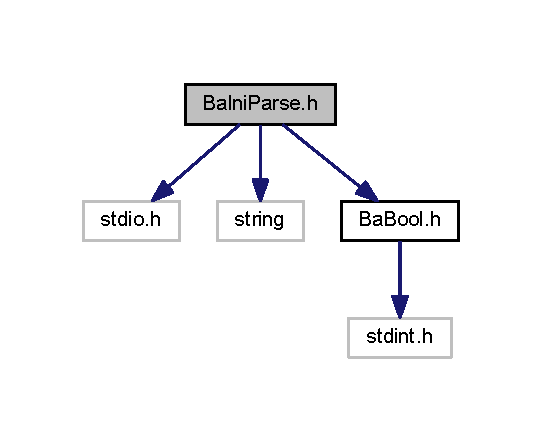
\includegraphics[width=260pt]{BaIniParse_8h__incl}
\end{center}
\end{figure}
\subsection*{Classes}
\begin{DoxyCompactItemize}
\item 
class \hyperlink{classIBaIniParser}{I\+Ba\+Ini\+Parser}
\begin{DoxyCompactList}\small\item\em I\+NI parser C++ interface. \end{DoxyCompactList}\end{DoxyCompactItemize}
\subsection*{Typedefs}
\begin{DoxyCompactItemize}
\item 
\mbox{\Hypertarget{BaIniParse_8h_a4aa7524aede4de49e1b9e3d9c4e4a6bc}\label{BaIniParse_8h_a4aa7524aede4de49e1b9e3d9c4e4a6bc}} 
typedef void $\ast$ \hyperlink{BaIniParse_8h_a4aa7524aede4de49e1b9e3d9c4e4a6bc}{T\+Ba\+Ini\+Parse\+Hdl}
\begin{DoxyCompactList}\small\item\em C I\+NI parser handle. \end{DoxyCompactList}\end{DoxyCompactItemize}
\subsection*{Functions}
\begin{DoxyCompactItemize}
\item 
\hyperlink{BaIniParse_8h_a4aa7524aede4de49e1b9e3d9c4e4a6bc}{T\+Ba\+Ini\+Parse\+Hdl} \hyperlink{BaIniParse_8h_a441bf1490f51fd14eb8429f00527e88e}{Ba\+Ini\+Parse\+Create} (const char $\ast$file)
\begin{DoxyCompactList}\small\item\em Create factory for an I\+NI parser. \end{DoxyCompactList}\item 
\hyperlink{BaBool_8h_a84d5a0de4729ca4c89f2479c605dbf3d}{T\+Ba\+Bool\+RC} \hyperlink{BaIniParse_8h_a0ffac10268e4667e5231e4d7c289315b}{Ba\+Ini\+Parse\+Destroy} (\hyperlink{BaIniParse_8h_a4aa7524aede4de49e1b9e3d9c4e4a6bc}{T\+Ba\+Ini\+Parse\+Hdl} hdl)
\begin{DoxyCompactList}\small\item\em Destroy and release resources of I\+NI parser. \end{DoxyCompactList}\item 
const char $\ast$ \hyperlink{BaIniParse_8h_a1211d49fa57e912fb47fc1f29d6ec666}{Ba\+Ini\+Parse\+Get\+String} (\hyperlink{BaIniParse_8h_a4aa7524aede4de49e1b9e3d9c4e4a6bc}{T\+Ba\+Ini\+Parse\+Hdl} hdl, const char $\ast$key, const char $\ast$def)
\begin{DoxyCompactList}\small\item\em Gets string value associated with a key or default if not found. \end{DoxyCompactList}\item 
int \hyperlink{BaIniParse_8h_abdf163061b63032b6d862e6c15a264b1}{Ba\+Ini\+Parse\+Get\+Int} (\hyperlink{BaIniParse_8h_a4aa7524aede4de49e1b9e3d9c4e4a6bc}{T\+Ba\+Ini\+Parse\+Hdl} hdl, const char $\ast$key, int def)
\begin{DoxyCompactList}\small\item\em Gets integer value associated with a key or default if not found or parse failed. \end{DoxyCompactList}\item 
double \hyperlink{BaIniParse_8h_af573c9d241b67f8fd8facc94f787a374}{Ba\+Ini\+Parse\+Get\+Double} (\hyperlink{BaIniParse_8h_a4aa7524aede4de49e1b9e3d9c4e4a6bc}{T\+Ba\+Ini\+Parse\+Hdl} hdl, const char $\ast$key, double def)
\begin{DoxyCompactList}\small\item\em Gets double value associated with a key or default if not found or parse failed. \end{DoxyCompactList}\item 
\hyperlink{BaBool_8h_a5fe1eb8d6ba045ac2251a8f369c2e7b6}{T\+Ba\+Bool} \hyperlink{BaIniParse_8h_a5a02622dba66acc86a5c92a73c229750}{Ba\+Ini\+Parse\+Get\+Bool} (\hyperlink{BaIniParse_8h_a4aa7524aede4de49e1b9e3d9c4e4a6bc}{T\+Ba\+Ini\+Parse\+Hdl} hdl, const char $\ast$key, \hyperlink{BaBool_8h_a5fe1eb8d6ba045ac2251a8f369c2e7b6}{T\+Ba\+Bool} def)
\begin{DoxyCompactList}\small\item\em Gets bool value associated with a key or default if not found or parse failed. \end{DoxyCompactList}\item 
\hyperlink{BaBool_8h_a84d5a0de4729ca4c89f2479c605dbf3d}{T\+Ba\+Bool\+RC} \hyperlink{BaIniParse_8h_a87077a113ba63b256fcfbbf0d1242797}{Ba\+Ini\+Parse\+Set} (\hyperlink{BaIniParse_8h_a4aa7524aede4de49e1b9e3d9c4e4a6bc}{T\+Ba\+Ini\+Parse\+Hdl} hdl, const char $\ast$key, const char $\ast$val)
\begin{DoxyCompactList}\small\item\em Add or overwrite a key-\/value pair. \end{DoxyCompactList}\item 
\hyperlink{BaBool_8h_a84d5a0de4729ca4c89f2479c605dbf3d}{T\+Ba\+Bool\+RC} \hyperlink{BaIniParse_8h_ae8e2fe9002a556cd48c55427da291479}{Ba\+Ini\+Parse\+Reset} (\hyperlink{BaIniParse_8h_a4aa7524aede4de49e1b9e3d9c4e4a6bc}{T\+Ba\+Ini\+Parse\+Hdl} hdl, const char $\ast$key)
\begin{DoxyCompactList}\small\item\em Reset or erase a key-\/value pair. \end{DoxyCompactList}\item 
\hyperlink{BaBool_8h_a5fe1eb8d6ba045ac2251a8f369c2e7b6}{T\+Ba\+Bool} \hyperlink{BaIniParse_8h_a8b195ded67f37d591e1b663383d327d5}{Ba\+Ini\+Parse\+Exists} (\hyperlink{BaIniParse_8h_a4aa7524aede4de49e1b9e3d9c4e4a6bc}{T\+Ba\+Ini\+Parse\+Hdl} hdl, const char $\ast$key)
\begin{DoxyCompactList}\small\item\em Gets if the entry exists. \end{DoxyCompactList}\item 
void \hyperlink{BaIniParse_8h_a30c3564a74b2ecaaac46348866bb3469}{Ba\+Ini\+Parse\+Dump\+Ini} (\hyperlink{BaIniParse_8h_a4aa7524aede4de49e1b9e3d9c4e4a6bc}{T\+Ba\+Ini\+Parse\+Hdl} hdl, F\+I\+LE $\ast$f)
\begin{DoxyCompactList}\small\item\em Dumps the entries in loadable I\+NI format. \end{DoxyCompactList}\item 
\hyperlink{BaBool_8h_a5fe1eb8d6ba045ac2251a8f369c2e7b6}{T\+Ba\+Bool} \hyperlink{BaIniParse_8h_ae81e8e51ad056d5d95935fa6088ce4b5}{Ba\+Ini\+Parse\+Dump\+Ini\+Sec} (\hyperlink{BaIniParse_8h_a4aa7524aede4de49e1b9e3d9c4e4a6bc}{T\+Ba\+Ini\+Parse\+Hdl} hdl, const char $\ast$sec, F\+I\+LE $\ast$f)
\begin{DoxyCompactList}\small\item\em Dump all entries in a particular section in loadable I\+NI format. \end{DoxyCompactList}\item 
\hyperlink{BaBool_8h_a5fe1eb8d6ba045ac2251a8f369c2e7b6}{T\+Ba\+Bool} \hyperlink{BaIniParse_8h_a93b569295cce8dded92c7f31ff5eeedc}{Ba\+Ini\+Parse\+Dump\+Ini\+Sec\+Less} (\hyperlink{BaIniParse_8h_a4aa7524aede4de49e1b9e3d9c4e4a6bc}{T\+Ba\+Ini\+Parse\+Hdl} hdl, F\+I\+LE $\ast$f)
\begin{DoxyCompactList}\small\item\em Dumps all section-\/less entries. \end{DoxyCompactList}\item 
void \hyperlink{BaIniParse_8h_a4b07cbe290b4c19c9902aceeb021837c}{Ba\+Ini\+Parse\+Dump} (\hyperlink{BaIniParse_8h_a4aa7524aede4de49e1b9e3d9c4e4a6bc}{T\+Ba\+Ini\+Parse\+Hdl} hdl, F\+I\+LE $\ast$f)
\begin{DoxyCompactList}\small\item\em Dumps all the raw entries in non-\/loadable format. \end{DoxyCompactList}\item 
\hyperlink{classIBaIniParser}{I\+Ba\+Ini\+Parser} $\ast$ \hyperlink{BaIniParse_8h_a20f257ac13e000d1b4451244173cdaf2}{I\+Ba\+Ini\+Parser\+Create} (const char $\ast$file)
\begin{DoxyCompactList}\small\item\em Create factory for an I\+NI parser. \end{DoxyCompactList}\item 
bool \hyperlink{BaIniParse_8h_ac602f997d7583090e6112abeba61d606}{I\+Ba\+Ini\+Parser\+Destroy} (\hyperlink{classIBaIniParser}{I\+Ba\+Ini\+Parser} $\ast$p\+Hdl)
\begin{DoxyCompactList}\small\item\em Destroy and release resources of I\+NI parser. \end{DoxyCompactList}\end{DoxyCompactItemize}


\subsection{Detailed Description}
Ini/config files parser based on iniparser from N. 

Devillard T\+O\+DO\+: Check if case insensitive is good 

\subsection{Function Documentation}
\mbox{\Hypertarget{BaIniParse_8h_a441bf1490f51fd14eb8429f00527e88e}\label{BaIniParse_8h_a441bf1490f51fd14eb8429f00527e88e}} 
\index{Ba\+Ini\+Parse.\+h@{Ba\+Ini\+Parse.\+h}!Ba\+Ini\+Parse\+Create@{Ba\+Ini\+Parse\+Create}}
\index{Ba\+Ini\+Parse\+Create@{Ba\+Ini\+Parse\+Create}!Ba\+Ini\+Parse.\+h@{Ba\+Ini\+Parse.\+h}}
\subsubsection{\texorpdfstring{Ba\+Ini\+Parse\+Create()}{BaIniParseCreate()}}
{\footnotesize\ttfamily \hyperlink{BaIniParse_8h_a4aa7524aede4de49e1b9e3d9c4e4a6bc}{T\+Ba\+Ini\+Parse\+Hdl} Ba\+Ini\+Parse\+Create (\begin{DoxyParamCaption}\item[{const char $\ast$}]{file }\end{DoxyParamCaption})}



Create factory for an I\+NI parser. 

If the file pointer is null it will be created with an empty dictionary. The data added to the dictionary can later be saved to disk with \hyperlink{BaIniParse_8h_a30c3564a74b2ecaaac46348866bb3469}{Ba\+Ini\+Parse\+Dump\+Ini}. \begin{DoxyReturn}{Returns}
Handle if success, otherwise, null 
\end{DoxyReturn}

\begin{DoxyParams}[1]{Parameters}
\mbox{\tt in}  & {\em file} & Path to file \\
\hline
\end{DoxyParams}
\mbox{\Hypertarget{BaIniParse_8h_a0ffac10268e4667e5231e4d7c289315b}\label{BaIniParse_8h_a0ffac10268e4667e5231e4d7c289315b}} 
\index{Ba\+Ini\+Parse.\+h@{Ba\+Ini\+Parse.\+h}!Ba\+Ini\+Parse\+Destroy@{Ba\+Ini\+Parse\+Destroy}}
\index{Ba\+Ini\+Parse\+Destroy@{Ba\+Ini\+Parse\+Destroy}!Ba\+Ini\+Parse.\+h@{Ba\+Ini\+Parse.\+h}}
\subsubsection{\texorpdfstring{Ba\+Ini\+Parse\+Destroy()}{BaIniParseDestroy()}}
{\footnotesize\ttfamily \hyperlink{BaBool_8h_a84d5a0de4729ca4c89f2479c605dbf3d}{T\+Ba\+Bool\+RC} Ba\+Ini\+Parse\+Destroy (\begin{DoxyParamCaption}\item[{\hyperlink{BaIniParse_8h_a4aa7524aede4de49e1b9e3d9c4e4a6bc}{T\+Ba\+Ini\+Parse\+Hdl}}]{hdl }\end{DoxyParamCaption})}



Destroy and release resources of I\+NI parser. 

\begin{DoxyReturn}{Returns}
True if success, otherwise, false 
\end{DoxyReturn}

\begin{DoxyParams}[1]{Parameters}
\mbox{\tt in}  & {\em hdl} & I\+NI parser handle to destroy \\
\hline
\end{DoxyParams}
\mbox{\Hypertarget{BaIniParse_8h_a1211d49fa57e912fb47fc1f29d6ec666}\label{BaIniParse_8h_a1211d49fa57e912fb47fc1f29d6ec666}} 
\index{Ba\+Ini\+Parse.\+h@{Ba\+Ini\+Parse.\+h}!Ba\+Ini\+Parse\+Get\+String@{Ba\+Ini\+Parse\+Get\+String}}
\index{Ba\+Ini\+Parse\+Get\+String@{Ba\+Ini\+Parse\+Get\+String}!Ba\+Ini\+Parse.\+h@{Ba\+Ini\+Parse.\+h}}
\subsubsection{\texorpdfstring{Ba\+Ini\+Parse\+Get\+String()}{BaIniParseGetString()}}
{\footnotesize\ttfamily const char$\ast$ Ba\+Ini\+Parse\+Get\+String (\begin{DoxyParamCaption}\item[{\hyperlink{BaIniParse_8h_a4aa7524aede4de49e1b9e3d9c4e4a6bc}{T\+Ba\+Ini\+Parse\+Hdl}}]{hdl,  }\item[{const char $\ast$}]{key,  }\item[{const char $\ast$}]{def }\end{DoxyParamCaption})}



Gets string value associated with a key or default if not found. 

\begin{DoxyReturn}{Returns}
the value or def. The returned string must not be edited or freed and invalidates if the instance handle is destroyed 
\end{DoxyReturn}

\begin{DoxyParams}[1]{Parameters}
\mbox{\tt in}  & {\em hdl} & Handle \\
\hline
\mbox{\tt in}  & {\em key} & Key as \char`\"{}section\+:key\char`\"{} \\
\hline
\mbox{\tt in}  & {\em def} & Default value to return if not found \\
\hline
\end{DoxyParams}
\mbox{\Hypertarget{BaIniParse_8h_abdf163061b63032b6d862e6c15a264b1}\label{BaIniParse_8h_abdf163061b63032b6d862e6c15a264b1}} 
\index{Ba\+Ini\+Parse.\+h@{Ba\+Ini\+Parse.\+h}!Ba\+Ini\+Parse\+Get\+Int@{Ba\+Ini\+Parse\+Get\+Int}}
\index{Ba\+Ini\+Parse\+Get\+Int@{Ba\+Ini\+Parse\+Get\+Int}!Ba\+Ini\+Parse.\+h@{Ba\+Ini\+Parse.\+h}}
\subsubsection{\texorpdfstring{Ba\+Ini\+Parse\+Get\+Int()}{BaIniParseGetInt()}}
{\footnotesize\ttfamily int Ba\+Ini\+Parse\+Get\+Int (\begin{DoxyParamCaption}\item[{\hyperlink{BaIniParse_8h_a4aa7524aede4de49e1b9e3d9c4e4a6bc}{T\+Ba\+Ini\+Parse\+Hdl}}]{hdl,  }\item[{const char $\ast$}]{key,  }\item[{int}]{def }\end{DoxyParamCaption})}



Gets integer value associated with a key or default if not found or parse failed. 

Supported values for integers include the usual C notation so decimal, octal (starting with 0) and hexadecimal (starting with 0x) are supported. Examples\+:
\begin{DoxyItemize}
\item \char`\"{}42\char`\"{} -\/$>$ 42
\item \char`\"{}042\char`\"{} -\/$>$ 34 (octal -\/$>$ decimal)
\item \char`\"{}0x42\char`\"{} -\/$>$ 66 (hexa -\/$>$ decimal)
\end{DoxyItemize}

\begin{DoxyReturn}{Returns}
the value or def 
\end{DoxyReturn}

\begin{DoxyParams}[1]{Parameters}
\mbox{\tt in}  & {\em hdl} & Handle \\
\hline
\mbox{\tt in}  & {\em key} & Key as \char`\"{}section\+:key\char`\"{} \\
\hline
\mbox{\tt in}  & {\em def} & Default value to return if not found \\
\hline
\end{DoxyParams}
\mbox{\Hypertarget{BaIniParse_8h_af573c9d241b67f8fd8facc94f787a374}\label{BaIniParse_8h_af573c9d241b67f8fd8facc94f787a374}} 
\index{Ba\+Ini\+Parse.\+h@{Ba\+Ini\+Parse.\+h}!Ba\+Ini\+Parse\+Get\+Double@{Ba\+Ini\+Parse\+Get\+Double}}
\index{Ba\+Ini\+Parse\+Get\+Double@{Ba\+Ini\+Parse\+Get\+Double}!Ba\+Ini\+Parse.\+h@{Ba\+Ini\+Parse.\+h}}
\subsubsection{\texorpdfstring{Ba\+Ini\+Parse\+Get\+Double()}{BaIniParseGetDouble()}}
{\footnotesize\ttfamily double Ba\+Ini\+Parse\+Get\+Double (\begin{DoxyParamCaption}\item[{\hyperlink{BaIniParse_8h_a4aa7524aede4de49e1b9e3d9c4e4a6bc}{T\+Ba\+Ini\+Parse\+Hdl}}]{hdl,  }\item[{const char $\ast$}]{key,  }\item[{double}]{def }\end{DoxyParamCaption})}



Gets double value associated with a key or default if not found or parse failed. 

Supported values for double include the usual C notation including the scientific notation. Examples\+:
\begin{DoxyItemize}
\item \char`\"{}3.\+14\char`\"{} -\/$>$ 3.\+14
\item \char`\"{}3.\+0e-\/3\char`\"{} -\/$>$ 0.\+003
\end{DoxyItemize}

\begin{DoxyReturn}{Returns}
the value or def 
\end{DoxyReturn}

\begin{DoxyParams}[1]{Parameters}
\mbox{\tt in}  & {\em hdl} & Handle \\
\hline
\mbox{\tt in}  & {\em key} & Key as \char`\"{}section\+:key\char`\"{} \\
\hline
\mbox{\tt in}  & {\em def} & Default value to return if not found \\
\hline
\end{DoxyParams}
\mbox{\Hypertarget{BaIniParse_8h_a5a02622dba66acc86a5c92a73c229750}\label{BaIniParse_8h_a5a02622dba66acc86a5c92a73c229750}} 
\index{Ba\+Ini\+Parse.\+h@{Ba\+Ini\+Parse.\+h}!Ba\+Ini\+Parse\+Get\+Bool@{Ba\+Ini\+Parse\+Get\+Bool}}
\index{Ba\+Ini\+Parse\+Get\+Bool@{Ba\+Ini\+Parse\+Get\+Bool}!Ba\+Ini\+Parse.\+h@{Ba\+Ini\+Parse.\+h}}
\subsubsection{\texorpdfstring{Ba\+Ini\+Parse\+Get\+Bool()}{BaIniParseGetBool()}}
{\footnotesize\ttfamily \hyperlink{BaBool_8h_a5fe1eb8d6ba045ac2251a8f369c2e7b6}{T\+Ba\+Bool} Ba\+Ini\+Parse\+Get\+Bool (\begin{DoxyParamCaption}\item[{\hyperlink{BaIniParse_8h_a4aa7524aede4de49e1b9e3d9c4e4a6bc}{T\+Ba\+Ini\+Parse\+Hdl}}]{hdl,  }\item[{const char $\ast$}]{key,  }\item[{\hyperlink{BaBool_8h_a5fe1eb8d6ba045ac2251a8f369c2e7b6}{T\+Ba\+Bool}}]{def }\end{DoxyParamCaption})}



Gets bool value associated with a key or default if not found or parse failed. 

A true is found if one of the following is matched\+:
\begin{DoxyItemize}
\item A string starting with \textquotesingle{}y\textquotesingle{}
\item A string starting with \textquotesingle{}Y\textquotesingle{}
\item A string starting with \textquotesingle{}t\textquotesingle{}
\item A string starting with \textquotesingle{}T\textquotesingle{}
\item A string starting with \textquotesingle{}1\textquotesingle{} A false is found if one of the following is matched\+:
\item A string starting with \textquotesingle{}n\textquotesingle{}
\item A string starting with \textquotesingle{}N\textquotesingle{}
\item A string starting with \textquotesingle{}f\textquotesingle{}
\item A string starting with \textquotesingle{}F\textquotesingle{}
\item A string starting with \textquotesingle{}0\textquotesingle{} \begin{DoxyReturn}{Returns}
the value or def 
\end{DoxyReturn}

\end{DoxyItemize}
\begin{DoxyParams}[1]{Parameters}
\mbox{\tt in}  & {\em hdl} & Handle \\
\hline
\mbox{\tt in}  & {\em key} & Key as \char`\"{}section\+:key\char`\"{} \\
\hline
\mbox{\tt in}  & {\em def} & Default value to return if not found \\
\hline
\end{DoxyParams}
\mbox{\Hypertarget{BaIniParse_8h_a87077a113ba63b256fcfbbf0d1242797}\label{BaIniParse_8h_a87077a113ba63b256fcfbbf0d1242797}} 
\index{Ba\+Ini\+Parse.\+h@{Ba\+Ini\+Parse.\+h}!Ba\+Ini\+Parse\+Set@{Ba\+Ini\+Parse\+Set}}
\index{Ba\+Ini\+Parse\+Set@{Ba\+Ini\+Parse\+Set}!Ba\+Ini\+Parse.\+h@{Ba\+Ini\+Parse.\+h}}
\subsubsection{\texorpdfstring{Ba\+Ini\+Parse\+Set()}{BaIniParseSet()}}
{\footnotesize\ttfamily \hyperlink{BaBool_8h_a84d5a0de4729ca4c89f2479c605dbf3d}{T\+Ba\+Bool\+RC} Ba\+Ini\+Parse\+Set (\begin{DoxyParamCaption}\item[{\hyperlink{BaIniParse_8h_a4aa7524aede4de49e1b9e3d9c4e4a6bc}{T\+Ba\+Ini\+Parse\+Hdl}}]{hdl,  }\item[{const char $\ast$}]{key,  }\item[{const char $\ast$}]{val }\end{DoxyParamCaption})}



Add or overwrite a key-\/value pair. 

\begin{DoxyReturn}{Returns}
Error or success 
\end{DoxyReturn}

\begin{DoxyParams}[1]{Parameters}
\mbox{\tt in}  & {\em hdl} & Handle \\
\hline
\mbox{\tt in}  & {\em key} & Key as \char`\"{}section\+:key\char`\"{} \\
\hline
\mbox{\tt in}  & {\em val} & Value \\
\hline
\end{DoxyParams}
\mbox{\Hypertarget{BaIniParse_8h_ae8e2fe9002a556cd48c55427da291479}\label{BaIniParse_8h_ae8e2fe9002a556cd48c55427da291479}} 
\index{Ba\+Ini\+Parse.\+h@{Ba\+Ini\+Parse.\+h}!Ba\+Ini\+Parse\+Reset@{Ba\+Ini\+Parse\+Reset}}
\index{Ba\+Ini\+Parse\+Reset@{Ba\+Ini\+Parse\+Reset}!Ba\+Ini\+Parse.\+h@{Ba\+Ini\+Parse.\+h}}
\subsubsection{\texorpdfstring{Ba\+Ini\+Parse\+Reset()}{BaIniParseReset()}}
{\footnotesize\ttfamily \hyperlink{BaBool_8h_a84d5a0de4729ca4c89f2479c605dbf3d}{T\+Ba\+Bool\+RC} Ba\+Ini\+Parse\+Reset (\begin{DoxyParamCaption}\item[{\hyperlink{BaIniParse_8h_a4aa7524aede4de49e1b9e3d9c4e4a6bc}{T\+Ba\+Ini\+Parse\+Hdl}}]{hdl,  }\item[{const char $\ast$}]{key }\end{DoxyParamCaption})}



Reset or erase a key-\/value pair. 

\begin{DoxyReturn}{Returns}
true if the element was erased 
\end{DoxyReturn}

\begin{DoxyParams}[1]{Parameters}
\mbox{\tt in}  & {\em hdl} & Handle \\
\hline
\mbox{\tt in}  & {\em key} & Key as \char`\"{}section\+:key\char`\"{} \\
\hline
\end{DoxyParams}
\mbox{\Hypertarget{BaIniParse_8h_a8b195ded67f37d591e1b663383d327d5}\label{BaIniParse_8h_a8b195ded67f37d591e1b663383d327d5}} 
\index{Ba\+Ini\+Parse.\+h@{Ba\+Ini\+Parse.\+h}!Ba\+Ini\+Parse\+Exists@{Ba\+Ini\+Parse\+Exists}}
\index{Ba\+Ini\+Parse\+Exists@{Ba\+Ini\+Parse\+Exists}!Ba\+Ini\+Parse.\+h@{Ba\+Ini\+Parse.\+h}}
\subsubsection{\texorpdfstring{Ba\+Ini\+Parse\+Exists()}{BaIniParseExists()}}
{\footnotesize\ttfamily \hyperlink{BaBool_8h_a5fe1eb8d6ba045ac2251a8f369c2e7b6}{T\+Ba\+Bool} Ba\+Ini\+Parse\+Exists (\begin{DoxyParamCaption}\item[{\hyperlink{BaIniParse_8h_a4aa7524aede4de49e1b9e3d9c4e4a6bc}{T\+Ba\+Ini\+Parse\+Hdl}}]{hdl,  }\item[{const char $\ast$}]{key }\end{DoxyParamCaption})}



Gets if the entry exists. 

\begin{DoxyReturn}{Returns}
True if entry exists 
\end{DoxyReturn}

\begin{DoxyParams}[1]{Parameters}
\mbox{\tt in}  & {\em hdl} & Handle \\
\hline
\mbox{\tt in}  & {\em key} & Key as \char`\"{}section\+:key\char`\"{} \\
\hline
\end{DoxyParams}
\mbox{\Hypertarget{BaIniParse_8h_a30c3564a74b2ecaaac46348866bb3469}\label{BaIniParse_8h_a30c3564a74b2ecaaac46348866bb3469}} 
\index{Ba\+Ini\+Parse.\+h@{Ba\+Ini\+Parse.\+h}!Ba\+Ini\+Parse\+Dump\+Ini@{Ba\+Ini\+Parse\+Dump\+Ini}}
\index{Ba\+Ini\+Parse\+Dump\+Ini@{Ba\+Ini\+Parse\+Dump\+Ini}!Ba\+Ini\+Parse.\+h@{Ba\+Ini\+Parse.\+h}}
\subsubsection{\texorpdfstring{Ba\+Ini\+Parse\+Dump\+Ini()}{BaIniParseDumpIni()}}
{\footnotesize\ttfamily void Ba\+Ini\+Parse\+Dump\+Ini (\begin{DoxyParamCaption}\item[{\hyperlink{BaIniParse_8h_a4aa7524aede4de49e1b9e3d9c4e4a6bc}{T\+Ba\+Ini\+Parse\+Hdl}}]{hdl,  }\item[{F\+I\+LE $\ast$}]{f }\end{DoxyParamCaption})}



Dumps the entries in loadable I\+NI format. 


\begin{DoxyParams}[1]{Parameters}
\mbox{\tt in}  & {\em hdl} & Handle \\
\hline
\mbox{\tt in}  & {\em f} & Opened output file (can also be stdout) \\
\hline
\end{DoxyParams}
\mbox{\Hypertarget{BaIniParse_8h_ae81e8e51ad056d5d95935fa6088ce4b5}\label{BaIniParse_8h_ae81e8e51ad056d5d95935fa6088ce4b5}} 
\index{Ba\+Ini\+Parse.\+h@{Ba\+Ini\+Parse.\+h}!Ba\+Ini\+Parse\+Dump\+Ini\+Sec@{Ba\+Ini\+Parse\+Dump\+Ini\+Sec}}
\index{Ba\+Ini\+Parse\+Dump\+Ini\+Sec@{Ba\+Ini\+Parse\+Dump\+Ini\+Sec}!Ba\+Ini\+Parse.\+h@{Ba\+Ini\+Parse.\+h}}
\subsubsection{\texorpdfstring{Ba\+Ini\+Parse\+Dump\+Ini\+Sec()}{BaIniParseDumpIniSec()}}
{\footnotesize\ttfamily \hyperlink{BaBool_8h_a5fe1eb8d6ba045ac2251a8f369c2e7b6}{T\+Ba\+Bool} Ba\+Ini\+Parse\+Dump\+Ini\+Sec (\begin{DoxyParamCaption}\item[{\hyperlink{BaIniParse_8h_a4aa7524aede4de49e1b9e3d9c4e4a6bc}{T\+Ba\+Ini\+Parse\+Hdl}}]{hdl,  }\item[{const char $\ast$}]{sec,  }\item[{F\+I\+LE $\ast$}]{f }\end{DoxyParamCaption})}



Dump all entries in a particular section in loadable I\+NI format. 

\begin{DoxyReturn}{Returns}
true if section exists 
\end{DoxyReturn}

\begin{DoxyParams}[1]{Parameters}
\mbox{\tt in}  & {\em hdl} & Handle \\
\hline
\mbox{\tt in}  & {\em sec} & Section name \\
\hline
\mbox{\tt in}  & {\em f} & Opened output file (can also be stdout) \\
\hline
\end{DoxyParams}
\mbox{\Hypertarget{BaIniParse_8h_a93b569295cce8dded92c7f31ff5eeedc}\label{BaIniParse_8h_a93b569295cce8dded92c7f31ff5eeedc}} 
\index{Ba\+Ini\+Parse.\+h@{Ba\+Ini\+Parse.\+h}!Ba\+Ini\+Parse\+Dump\+Ini\+Sec\+Less@{Ba\+Ini\+Parse\+Dump\+Ini\+Sec\+Less}}
\index{Ba\+Ini\+Parse\+Dump\+Ini\+Sec\+Less@{Ba\+Ini\+Parse\+Dump\+Ini\+Sec\+Less}!Ba\+Ini\+Parse.\+h@{Ba\+Ini\+Parse.\+h}}
\subsubsection{\texorpdfstring{Ba\+Ini\+Parse\+Dump\+Ini\+Sec\+Less()}{BaIniParseDumpIniSecLess()}}
{\footnotesize\ttfamily \hyperlink{BaBool_8h_a5fe1eb8d6ba045ac2251a8f369c2e7b6}{T\+Ba\+Bool} Ba\+Ini\+Parse\+Dump\+Ini\+Sec\+Less (\begin{DoxyParamCaption}\item[{\hyperlink{BaIniParse_8h_a4aa7524aede4de49e1b9e3d9c4e4a6bc}{T\+Ba\+Ini\+Parse\+Hdl}}]{hdl,  }\item[{F\+I\+LE $\ast$}]{f }\end{DoxyParamCaption})}



Dumps all section-\/less entries. 

\begin{DoxyReturn}{Returns}
true if section exists 
\end{DoxyReturn}

\begin{DoxyParams}[1]{Parameters}
\mbox{\tt in}  & {\em hdl} & Handle \\
\hline
\mbox{\tt in}  & {\em f} & Opened output file (can also be stdout) \\
\hline
\end{DoxyParams}
\mbox{\Hypertarget{BaIniParse_8h_a4b07cbe290b4c19c9902aceeb021837c}\label{BaIniParse_8h_a4b07cbe290b4c19c9902aceeb021837c}} 
\index{Ba\+Ini\+Parse.\+h@{Ba\+Ini\+Parse.\+h}!Ba\+Ini\+Parse\+Dump@{Ba\+Ini\+Parse\+Dump}}
\index{Ba\+Ini\+Parse\+Dump@{Ba\+Ini\+Parse\+Dump}!Ba\+Ini\+Parse.\+h@{Ba\+Ini\+Parse.\+h}}
\subsubsection{\texorpdfstring{Ba\+Ini\+Parse\+Dump()}{BaIniParseDump()}}
{\footnotesize\ttfamily void Ba\+Ini\+Parse\+Dump (\begin{DoxyParamCaption}\item[{\hyperlink{BaIniParse_8h_a4aa7524aede4de49e1b9e3d9c4e4a6bc}{T\+Ba\+Ini\+Parse\+Hdl}}]{hdl,  }\item[{F\+I\+LE $\ast$}]{f }\end{DoxyParamCaption})}



Dumps all the raw entries in non-\/loadable format. 


\begin{DoxyParams}[1]{Parameters}
\mbox{\tt in}  & {\em hdl} & Handle \\
\hline
\mbox{\tt in}  & {\em f} & Opened output file (can also be stdout) \\
\hline
\end{DoxyParams}
\mbox{\Hypertarget{BaIniParse_8h_a20f257ac13e000d1b4451244173cdaf2}\label{BaIniParse_8h_a20f257ac13e000d1b4451244173cdaf2}} 
\index{Ba\+Ini\+Parse.\+h@{Ba\+Ini\+Parse.\+h}!I\+Ba\+Ini\+Parser\+Create@{I\+Ba\+Ini\+Parser\+Create}}
\index{I\+Ba\+Ini\+Parser\+Create@{I\+Ba\+Ini\+Parser\+Create}!Ba\+Ini\+Parse.\+h@{Ba\+Ini\+Parse.\+h}}
\subsubsection{\texorpdfstring{I\+Ba\+Ini\+Parser\+Create()}{IBaIniParserCreate()}}
{\footnotesize\ttfamily \hyperlink{classIBaIniParser}{I\+Ba\+Ini\+Parser}$\ast$ I\+Ba\+Ini\+Parser\+Create (\begin{DoxyParamCaption}\item[{const char $\ast$}]{file }\end{DoxyParamCaption})}



Create factory for an I\+NI parser. 

If the file pointer is null it will be created with an empty dictionary. The data added to the dictionary can later be saved to disk with \hyperlink{classIBaIniParser_ac7c44f2ec3373a93f69bd4a465cfa2a7}{I\+Ba\+Ini\+Parser\+::\+Dump\+Ini()}. \begin{DoxyReturn}{Returns}
Handle if success, otherwise, null 
\end{DoxyReturn}

\begin{DoxyParams}[1]{Parameters}
\mbox{\tt in}  & {\em file} & Path to file \\
\hline
\end{DoxyParams}
\mbox{\Hypertarget{BaIniParse_8h_ac602f997d7583090e6112abeba61d606}\label{BaIniParse_8h_ac602f997d7583090e6112abeba61d606}} 
\index{Ba\+Ini\+Parse.\+h@{Ba\+Ini\+Parse.\+h}!I\+Ba\+Ini\+Parser\+Destroy@{I\+Ba\+Ini\+Parser\+Destroy}}
\index{I\+Ba\+Ini\+Parser\+Destroy@{I\+Ba\+Ini\+Parser\+Destroy}!Ba\+Ini\+Parse.\+h@{Ba\+Ini\+Parse.\+h}}
\subsubsection{\texorpdfstring{I\+Ba\+Ini\+Parser\+Destroy()}{IBaIniParserDestroy()}}
{\footnotesize\ttfamily bool I\+Ba\+Ini\+Parser\+Destroy (\begin{DoxyParamCaption}\item[{\hyperlink{classIBaIniParser}{I\+Ba\+Ini\+Parser} $\ast$}]{p\+Hdl }\end{DoxyParamCaption})}



Destroy and release resources of I\+NI parser. 

\begin{DoxyReturn}{Returns}
True if success, otherwise, false 
\end{DoxyReturn}

\begin{DoxyParams}[1]{Parameters}
\mbox{\tt in}  & {\em p\+Hdl} & I\+NI parser handle to destroy \\
\hline
\end{DoxyParams}

\hypertarget{BaLog_8h}{}\section{Ba\+Log.\+h File Reference}
\label{BaLog_8h}\index{Ba\+Log.\+h@{Ba\+Log.\+h}}


...  




\subsection{Detailed Description}
... 


\hypertarget{BaLogMacros_8h}{}\section{Ba\+Log\+Macros.\+h File Reference}
\label{BaLogMacros_8h}\index{Ba\+Log\+Macros.\+h@{Ba\+Log\+Macros.\+h}}


This header defines macros for logging more easily.  


{\ttfamily \#include \char`\"{}Base\+Api.\+h\char`\"{}}\newline
Include dependency graph for Ba\+Log\+Macros.\+h\+:
\nopagebreak
\begin{figure}[H]
\begin{center}
\leavevmode
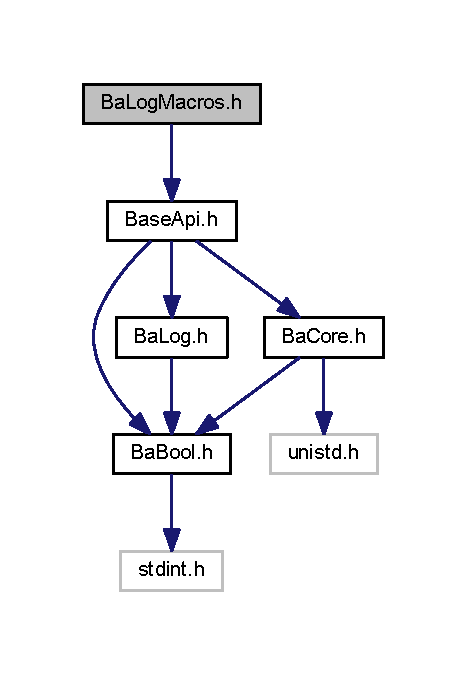
\includegraphics[width=224pt]{BaLogMacros_8h__incl}
\end{center}
\end{figure}
\subsection*{Macros}
\begin{Indent}\textbf{ Log Macros}\par
\begin{DoxyCompactItemize}
\item 
\#define \hyperlink{BaLogMacros_8h_af8f8c4db8a1f6b3502d826cdd2e8de52}{T\+R\+A\+C\+E\+\_\+}(fmt, ...)~\hyperlink{BaseApi_8h_a1914573ea9bce1d0ebe2c6ed0ac0ec2b}{Ba\+Api\+LogF}(\hyperlink{BaLog_8h_ab14f00a81932b8b62d2e8c4a2d7e3916a5109ed3aaf795c26ad4a42c30b658a02}{e\+Ba\+Log\+Prio\+\_\+\+Trace}, T\+AG, fmt, \#\#\+\_\+\+\_\+\+V\+A\+\_\+\+A\+R\+G\+S\+\_\+\+\_\+)
\begin{DoxyCompactList}\small\item\em Log with the given priority analog to {\ttfamily printf()} family. \end{DoxyCompactList}\item 
\#define \hyperlink{BaLogMacros_8h_afad173763727543cf4e09b6fb98046d0}{W\+A\+R\+N\+\_\+}(fmt, ...)~\hyperlink{BaseApi_8h_a1914573ea9bce1d0ebe2c6ed0ac0ec2b}{Ba\+Api\+LogF}(\hyperlink{BaLog_8h_ab14f00a81932b8b62d2e8c4a2d7e3916af0ab8313b1b5d47e5a9e2c405a7e1996}{e\+Ba\+Log\+Prio\+\_\+\+Warning}, T\+AG, fmt, \#\#\+\_\+\+\_\+\+V\+A\+\_\+\+A\+R\+G\+S\+\_\+\+\_\+)
\begin{DoxyCompactList}\small\item\em Log with the given priority analog to {\ttfamily printf()} family. \end{DoxyCompactList}\item 
\#define \hyperlink{BaLogMacros_8h_a6032afff6465e251362043298d374c8e}{E\+R\+R\+O\+R\+\_\+}(fmt, ...)~\hyperlink{BaseApi_8h_a1914573ea9bce1d0ebe2c6ed0ac0ec2b}{Ba\+Api\+LogF}(\hyperlink{BaLog_8h_ab14f00a81932b8b62d2e8c4a2d7e3916affcbdec070a745bc0b4a7ecd7bd2884f}{e\+Ba\+Log\+Prio\+\_\+\+Error}, T\+AG, fmt, \#\#\+\_\+\+\_\+\+V\+A\+\_\+\+A\+R\+G\+S\+\_\+\+\_\+)
\begin{DoxyCompactList}\small\item\em Log with the given priority analog to {\ttfamily printf()} family. \end{DoxyCompactList}\end{DoxyCompactItemize}
\end{Indent}


\subsection{Detailed Description}
This header defines macros for logging more easily. 

They expect that T\+AG is previously defined 

\subsection{Macro Definition Documentation}
\mbox{\Hypertarget{BaLogMacros_8h_af8f8c4db8a1f6b3502d826cdd2e8de52}\label{BaLogMacros_8h_af8f8c4db8a1f6b3502d826cdd2e8de52}} 
\index{Ba\+Log\+Macros.\+h@{Ba\+Log\+Macros.\+h}!T\+R\+A\+C\+E\+\_\+@{T\+R\+A\+C\+E\+\_\+}}
\index{T\+R\+A\+C\+E\+\_\+@{T\+R\+A\+C\+E\+\_\+}!Ba\+Log\+Macros.\+h@{Ba\+Log\+Macros.\+h}}
\subsubsection{\texorpdfstring{T\+R\+A\+C\+E\+\_\+}{TRACE\_}}
{\footnotesize\ttfamily \#define T\+R\+A\+C\+E\+\_\+(\begin{DoxyParamCaption}\item[{}]{fmt,  }\item[{}]{... }\end{DoxyParamCaption})~\hyperlink{BaseApi_8h_a1914573ea9bce1d0ebe2c6ed0ac0ec2b}{Ba\+Api\+LogF}(\hyperlink{BaLog_8h_ab14f00a81932b8b62d2e8c4a2d7e3916a5109ed3aaf795c26ad4a42c30b658a02}{e\+Ba\+Log\+Prio\+\_\+\+Trace}, T\+AG, fmt, \#\#\+\_\+\+\_\+\+V\+A\+\_\+\+A\+R\+G\+S\+\_\+\+\_\+)}



Log with the given priority analog to {\ttfamily printf()} family. 

This assumes that T\+AG is defined. see {\ttfamily \hyperlink{BaseApi_8h_a1914573ea9bce1d0ebe2c6ed0ac0ec2b}{Ba\+Api\+Log\+F()}} \mbox{\Hypertarget{BaLogMacros_8h_afad173763727543cf4e09b6fb98046d0}\label{BaLogMacros_8h_afad173763727543cf4e09b6fb98046d0}} 
\index{Ba\+Log\+Macros.\+h@{Ba\+Log\+Macros.\+h}!W\+A\+R\+N\+\_\+@{W\+A\+R\+N\+\_\+}}
\index{W\+A\+R\+N\+\_\+@{W\+A\+R\+N\+\_\+}!Ba\+Log\+Macros.\+h@{Ba\+Log\+Macros.\+h}}
\subsubsection{\texorpdfstring{W\+A\+R\+N\+\_\+}{WARN\_}}
{\footnotesize\ttfamily \#define W\+A\+R\+N\+\_\+(\begin{DoxyParamCaption}\item[{}]{fmt,  }\item[{}]{... }\end{DoxyParamCaption})~\hyperlink{BaseApi_8h_a1914573ea9bce1d0ebe2c6ed0ac0ec2b}{Ba\+Api\+LogF}(\hyperlink{BaLog_8h_ab14f00a81932b8b62d2e8c4a2d7e3916af0ab8313b1b5d47e5a9e2c405a7e1996}{e\+Ba\+Log\+Prio\+\_\+\+Warning}, T\+AG, fmt, \#\#\+\_\+\+\_\+\+V\+A\+\_\+\+A\+R\+G\+S\+\_\+\+\_\+)}



Log with the given priority analog to {\ttfamily printf()} family. 

This assumes that T\+AG is defined. see {\ttfamily \hyperlink{BaseApi_8h_a1914573ea9bce1d0ebe2c6ed0ac0ec2b}{Ba\+Api\+Log\+F()}} \mbox{\Hypertarget{BaLogMacros_8h_a6032afff6465e251362043298d374c8e}\label{BaLogMacros_8h_a6032afff6465e251362043298d374c8e}} 
\index{Ba\+Log\+Macros.\+h@{Ba\+Log\+Macros.\+h}!E\+R\+R\+O\+R\+\_\+@{E\+R\+R\+O\+R\+\_\+}}
\index{E\+R\+R\+O\+R\+\_\+@{E\+R\+R\+O\+R\+\_\+}!Ba\+Log\+Macros.\+h@{Ba\+Log\+Macros.\+h}}
\subsubsection{\texorpdfstring{E\+R\+R\+O\+R\+\_\+}{ERROR\_}}
{\footnotesize\ttfamily \#define E\+R\+R\+O\+R\+\_\+(\begin{DoxyParamCaption}\item[{}]{fmt,  }\item[{}]{... }\end{DoxyParamCaption})~\hyperlink{BaseApi_8h_a1914573ea9bce1d0ebe2c6ed0ac0ec2b}{Ba\+Api\+LogF}(\hyperlink{BaLog_8h_ab14f00a81932b8b62d2e8c4a2d7e3916affcbdec070a745bc0b4a7ecd7bd2884f}{e\+Ba\+Log\+Prio\+\_\+\+Error}, T\+AG, fmt, \#\#\+\_\+\+\_\+\+V\+A\+\_\+\+A\+R\+G\+S\+\_\+\+\_\+)}



Log with the given priority analog to {\ttfamily printf()} family. 

This assumes that T\+AG is defined. see {\ttfamily \hyperlink{BaseApi_8h_a1914573ea9bce1d0ebe2c6ed0ac0ec2b}{Ba\+Api\+Log\+F()}} 
\hypertarget{BaMsg_8h}{}\section{Ba\+Msg.\+h File Reference}
\label{BaMsg_8h}\index{Ba\+Msg.\+h@{Ba\+Msg.\+h}}


A\+P\+I for messages with state.  


{\ttfamily \#include \char`\"{}Ba\+Log.\+h\char`\"{}}\\*
Include dependency graph for Ba\+Msg.\+h\+:\nopagebreak
\begin{figure}[H]
\begin{center}
\leavevmode
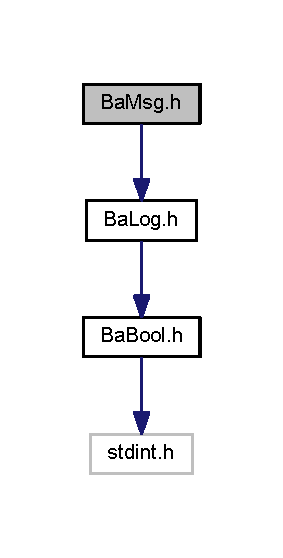
\includegraphics[width=136pt]{BaMsg_8h__incl}
\end{center}
\end{figure}
\subsection*{Macros}
\begin{DoxyCompactItemize}
\item 
\hypertarget{BaMsg_8h_a5ddf02d5c03db476fd91d87b1e3a8e6e}{}\#define \hyperlink{BaMsg_8h_a5ddf02d5c03db476fd91d87b1e3a8e6e}{B\+A\+M\+S\+G\+S\+E\+T\+S\+Y\+S\+L\+O\+G\+F}(log,  tag,  fmt, ...)~\hyperlink{BaMsg_8h_ab285acd845753344b3da6db1e60c80a2}{Ba\+Msg\+Set\+Sys\+Log\+F}(log, tag, \+\_\+\+\_\+\+L\+I\+N\+E\+\_\+\+\_\+, fmt, \+\_\+\+\_\+\+V\+A\+\_\+\+A\+R\+G\+S\+\_\+\+\_\+)\label{BaMsg_8h_a5ddf02d5c03db476fd91d87b1e3a8e6e}

\begin{DoxyCompactList}\small\item\em Syslog macro for C A\+P\+I. \end{DoxyCompactList}\item 
\hypertarget{BaMsg_8h_a79951ff6b5999141a69a4c6cbb32478a}{}\#define \hyperlink{BaMsg_8h_a79951ff6b5999141a69a4c6cbb32478a}{B\+A\+M\+S\+G\+S\+E\+T\+S\+Y\+S\+L\+O\+G}(log,  tag,  msg)~\hyperlink{BaMsg_8h_ae73c6be7d2b46e617ab2d2c222094b1f}{Ba\+Msg\+Set\+Sys\+Log}(log, tag, \+\_\+\+\_\+\+L\+I\+N\+E\+\_\+\+\_\+, msg)\label{BaMsg_8h_a79951ff6b5999141a69a4c6cbb32478a}

\begin{DoxyCompactList}\small\item\em Syslog macro for C A\+P\+I. \end{DoxyCompactList}\item 
\hypertarget{BaMsg_8h_a7758072566268146bb4c3171c6174afb}{}\#define \hyperlink{BaMsg_8h_a7758072566268146bb4c3171c6174afb}{I\+B\+A\+M\+S\+G\+S\+E\+T\+S\+Y\+S\+L\+O\+G\+F}(tag,  fmt, ...)~Set\+Sys\+Log\+F(tag, \+\_\+\+\_\+\+L\+I\+N\+E\+\_\+\+\_\+, fmt, \+\_\+\+\_\+\+V\+A\+\_\+\+A\+R\+G\+S\+\_\+\+\_\+)\label{BaMsg_8h_a7758072566268146bb4c3171c6174afb}

\begin{DoxyCompactList}\small\item\em Syslog macro for C++ A\+P\+I. \end{DoxyCompactList}\item 
\hypertarget{BaMsg_8h_a6210311bfa675d85ec0d390244b4b2f0}{}\#define \hyperlink{BaMsg_8h_a6210311bfa675d85ec0d390244b4b2f0}{I\+B\+A\+M\+S\+G\+S\+E\+T\+S\+Y\+S\+L\+O\+G}(tag,  msg)~Set\+Sys\+Log(tag, \+\_\+\+\_\+\+L\+I\+N\+E\+\_\+\+\_\+, msg)\label{BaMsg_8h_a6210311bfa675d85ec0d390244b4b2f0}

\begin{DoxyCompactList}\small\item\em Syslog macro for C++ A\+P\+I. \end{DoxyCompactList}\end{DoxyCompactItemize}
\subsection*{Typedefs}
\begin{DoxyCompactItemize}
\item 
\hypertarget{BaMsg_8h_aafa53fd0800007ea7994e44ad13a887a}{}typedef void $\ast$ \hyperlink{BaMsg_8h_aafa53fd0800007ea7994e44ad13a887a}{T\+Ba\+Msg\+Hdl}\label{BaMsg_8h_aafa53fd0800007ea7994e44ad13a887a}

\begin{DoxyCompactList}\small\item\em C message handle. \end{DoxyCompactList}\end{DoxyCompactItemize}
\subsection*{Functions}
\begin{Indent}{\bf Factory}\par
\begin{DoxyCompactItemize}
\item 
\hyperlink{BaMsg_8h_aafa53fd0800007ea7994e44ad13a887a}{T\+Ba\+Msg\+Hdl} \hyperlink{BaMsg_8h_a747950cb6c947a1b8f87d7b24f9dffb0}{Ba\+Msg\+Create} ()
\begin{DoxyCompactList}\small\item\em Create factory for a message with state. \end{DoxyCompactList}\item 
\hyperlink{BaBool_8h_a84d5a0de4729ca4c89f2479c605dbf3d}{T\+Ba\+Bool\+R\+C} \hyperlink{BaMsg_8h_aff9865961ff4eac198947bbca0f57bc2}{Ba\+Msg\+Destroy} (\hyperlink{BaMsg_8h_aafa53fd0800007ea7994e44ad13a887a}{T\+Ba\+Msg\+Hdl} hdl)
\begin{DoxyCompactList}\small\item\em Destroy and release resources of message with state. \end{DoxyCompactList}\end{DoxyCompactItemize}
\end{Indent}
\begin{Indent}{\bf Set to console}\par
\begin{DoxyCompactItemize}
\item 
void \hyperlink{BaMsg_8h_aa8eb770fb5565bdaea8e6f8d6abac22d}{Ba\+Msg\+Set\+Print\+F} (\hyperlink{BaMsg_8h_aafa53fd0800007ea7994e44ad13a887a}{T\+Ba\+Msg\+Hdl} hdl, const char $\ast$fmt,...)
\begin{DoxyCompactList}\small\item\em Prints a message to the console with state. \end{DoxyCompactList}\item 
void \hyperlink{BaMsg_8h_a947780e175568fa8f12109a1ca743ded}{Ba\+Msg\+Set\+Print} (\hyperlink{BaMsg_8h_aafa53fd0800007ea7994e44ad13a887a}{T\+Ba\+Msg\+Hdl} hdl, const char $\ast$msg)
\begin{DoxyCompactList}\small\item\em Prints a message to the console with state. \end{DoxyCompactList}\end{DoxyCompactItemize}
\end{Indent}
\begin{Indent}{\bf Set to syslog}\par
\begin{DoxyCompactItemize}
\item 
void \hyperlink{BaMsg_8h_ab285acd845753344b3da6db1e60c80a2}{Ba\+Msg\+Set\+Sys\+Log\+F} (\hyperlink{BaMsg_8h_aafa53fd0800007ea7994e44ad13a887a}{T\+Ba\+Msg\+Hdl} hdl, const char $\ast$tag, int line, const char $\ast$fmt,...)
\begin{DoxyCompactList}\small\item\em Logs a message to the syslog with state and maximum length of 65534 chars. \end{DoxyCompactList}\item 
void \hyperlink{BaMsg_8h_ae73c6be7d2b46e617ab2d2c222094b1f}{Ba\+Msg\+Set\+Sys\+Log} (\hyperlink{BaMsg_8h_aafa53fd0800007ea7994e44ad13a887a}{T\+Ba\+Msg\+Hdl} hdl, const char $\ast$tag, int line, const char $\ast$msg)
\begin{DoxyCompactList}\small\item\em Logs a message to the syslog with state and maximum length of 65534 chars. \end{DoxyCompactList}\end{DoxyCompactItemize}
\end{Indent}
\begin{Indent}{\bf Set to log}\par
\begin{DoxyCompactItemize}
\item 
void \hyperlink{BaMsg_8h_aa5c9afb0933a7a21900ae19bd319bb13}{Ba\+Msg\+Set\+Log\+F} (\hyperlink{BaMsg_8h_aafa53fd0800007ea7994e44ad13a887a}{T\+Ba\+Msg\+Hdl} hdl, \hyperlink{BaLog_8h_aafc4e99ec41825c3604bc4995a45b315}{T\+Ba\+Log\+Hdl} log, \hyperlink{BaLog_8h_ab14f00a81932b8b62d2e8c4a2d7e3916}{E\+Ba\+Log\+Prio} prio, const char $\ast$tag, const char $\ast$fmt,...)
\begin{DoxyCompactList}\small\item\em Logs a message to {\ttfamily p\+Log} with state and maximum length of 65534 chars. \end{DoxyCompactList}\item 
void \hyperlink{BaMsg_8h_ab8f315eeec9e46af1e6e515caee7b991}{Ba\+Msg\+Set\+Log} (\hyperlink{BaMsg_8h_aafa53fd0800007ea7994e44ad13a887a}{T\+Ba\+Msg\+Hdl} hdl, \hyperlink{BaLog_8h_aafc4e99ec41825c3604bc4995a45b315}{T\+Ba\+Log\+Hdl} log, \hyperlink{BaLog_8h_ab14f00a81932b8b62d2e8c4a2d7e3916}{E\+Ba\+Log\+Prio} prio, const char $\ast$tag, const char $\ast$msg)
\begin{DoxyCompactList}\small\item\em Logs a message to {\ttfamily p\+Log} with state and maximum length of 65534 chars. \end{DoxyCompactList}\end{DoxyCompactItemize}
\end{Indent}
\begin{Indent}{\bf Get, reset}\par
\begin{DoxyCompactItemize}
\item 
void \hyperlink{BaMsg_8h_a3a1e777dc423ee4faabffc481d4ab715}{Ba\+Msg\+Reset} (\hyperlink{BaMsg_8h_aafa53fd0800007ea7994e44ad13a887a}{T\+Ba\+Msg\+Hdl} hdl)
\begin{DoxyCompactList}\small\item\em Reset a set message. \end{DoxyCompactList}\item 
\hyperlink{BaBool_8h_a5fe1eb8d6ba045ac2251a8f369c2e7b6}{T\+Ba\+Bool} \hyperlink{BaMsg_8h_a97a02ca07716761fa22be88b52314a76}{Ba\+Msg\+Get} (\hyperlink{BaMsg_8h_aafa53fd0800007ea7994e44ad13a887a}{T\+Ba\+Msg\+Hdl} hdl)
\begin{DoxyCompactList}\small\item\em Get the state of the message. \end{DoxyCompactList}\end{DoxyCompactItemize}
\end{Indent}
\begin{Indent}{\bf C++ Factory}\par
\begin{DoxyCompactItemize}
\item 
I\+Ba\+Msg $\ast$ \hyperlink{BaMsg_8h_a4abd8e9092520542acb0a246d1454c67}{I\+Ba\+Msg\+Create} ()
\begin{DoxyCompactList}\small\item\em Create factory for a message with state. \end{DoxyCompactList}\item 
\hyperlink{BaBool_8h_a84d5a0de4729ca4c89f2479c605dbf3d}{T\+Ba\+Bool\+R\+C} \hyperlink{BaMsg_8h_a051e0750bf7aaa7339cffe55253dee36}{I\+Ba\+Msg\+Destroy} (I\+Ba\+Msg $\ast$p\+Hdl)
\begin{DoxyCompactList}\small\item\em Destroy and release resources of Message with state. \end{DoxyCompactList}\end{DoxyCompactItemize}
\end{Indent}


\subsection{Detailed Description}
A\+P\+I for messages with state. 

A message with state can be set and reset. If it is set, it cannot be set again before reseting it. These messages are mainly used to avoid cyclic messages. 

\subsection{Function Documentation}
\hypertarget{BaMsg_8h_a747950cb6c947a1b8f87d7b24f9dffb0}{}\index{Ba\+Msg.\+h@{Ba\+Msg.\+h}!Ba\+Msg\+Create@{Ba\+Msg\+Create}}
\index{Ba\+Msg\+Create@{Ba\+Msg\+Create}!Ba\+Msg.\+h@{Ba\+Msg.\+h}}
\subsubsection[{Ba\+Msg\+Create()}]{\setlength{\rightskip}{0pt plus 5cm}{\bf T\+Ba\+Msg\+Hdl} Ba\+Msg\+Create (
\begin{DoxyParamCaption}
{}
\end{DoxyParamCaption}
)}\label{BaMsg_8h_a747950cb6c947a1b8f87d7b24f9dffb0}


Create factory for a message with state. 

\begin{DoxyReturn}{Returns}
Handle if success, otherwise, null 
\end{DoxyReturn}
\hypertarget{BaMsg_8h_aff9865961ff4eac198947bbca0f57bc2}{}\index{Ba\+Msg.\+h@{Ba\+Msg.\+h}!Ba\+Msg\+Destroy@{Ba\+Msg\+Destroy}}
\index{Ba\+Msg\+Destroy@{Ba\+Msg\+Destroy}!Ba\+Msg.\+h@{Ba\+Msg.\+h}}
\subsubsection[{Ba\+Msg\+Destroy(\+T\+Ba\+Msg\+Hdl hdl)}]{\setlength{\rightskip}{0pt plus 5cm}{\bf T\+Ba\+Bool\+R\+C} Ba\+Msg\+Destroy (
\begin{DoxyParamCaption}
\item[{{\bf T\+Ba\+Msg\+Hdl}}]{hdl}
\end{DoxyParamCaption}
)}\label{BaMsg_8h_aff9865961ff4eac198947bbca0f57bc2}


Destroy and release resources of message with state. 

\begin{DoxyReturn}{Returns}
True if success, otherwise, false 
\end{DoxyReturn}

\begin{DoxyParams}[1]{Parameters}
\mbox{\tt in}  & {\em hdl} & Ba\+Log handle to destroy \\
\hline
\end{DoxyParams}
\hypertarget{BaMsg_8h_aa8eb770fb5565bdaea8e6f8d6abac22d}{}\index{Ba\+Msg.\+h@{Ba\+Msg.\+h}!Ba\+Msg\+Set\+Print\+F@{Ba\+Msg\+Set\+Print\+F}}
\index{Ba\+Msg\+Set\+Print\+F@{Ba\+Msg\+Set\+Print\+F}!Ba\+Msg.\+h@{Ba\+Msg.\+h}}
\subsubsection[{Ba\+Msg\+Set\+Print\+F(\+T\+Ba\+Msg\+Hdl hdl, const char $\ast$fmt,...)}]{\setlength{\rightskip}{0pt plus 5cm}void Ba\+Msg\+Set\+Print\+F (
\begin{DoxyParamCaption}
\item[{{\bf T\+Ba\+Msg\+Hdl}}]{hdl, }
\item[{const char $\ast$}]{fmt, }
\item[{}]{...}
\end{DoxyParamCaption}
)}\label{BaMsg_8h_aa8eb770fb5565bdaea8e6f8d6abac22d}


Prints a message to the console with state. 


\begin{DoxyParams}[1]{Parameters}
\mbox{\tt in}  & {\em hdl} & Handle \\
\hline
\mbox{\tt in}  & {\em fmt} & Message format \\
\hline
\end{DoxyParams}
\hypertarget{BaMsg_8h_a947780e175568fa8f12109a1ca743ded}{}\index{Ba\+Msg.\+h@{Ba\+Msg.\+h}!Ba\+Msg\+Set\+Print@{Ba\+Msg\+Set\+Print}}
\index{Ba\+Msg\+Set\+Print@{Ba\+Msg\+Set\+Print}!Ba\+Msg.\+h@{Ba\+Msg.\+h}}
\subsubsection[{Ba\+Msg\+Set\+Print(\+T\+Ba\+Msg\+Hdl hdl, const char $\ast$msg)}]{\setlength{\rightskip}{0pt plus 5cm}void Ba\+Msg\+Set\+Print (
\begin{DoxyParamCaption}
\item[{{\bf T\+Ba\+Msg\+Hdl}}]{hdl, }
\item[{const char $\ast$}]{msg}
\end{DoxyParamCaption}
)}\label{BaMsg_8h_a947780e175568fa8f12109a1ca743ded}


Prints a message to the console with state. 


\begin{DoxyParams}[1]{Parameters}
\mbox{\tt in}  & {\em hdl} & Handle \\
\hline
\mbox{\tt in}  & {\em msg} & Message format \\
\hline
\end{DoxyParams}
\hypertarget{BaMsg_8h_ab285acd845753344b3da6db1e60c80a2}{}\index{Ba\+Msg.\+h@{Ba\+Msg.\+h}!Ba\+Msg\+Set\+Sys\+Log\+F@{Ba\+Msg\+Set\+Sys\+Log\+F}}
\index{Ba\+Msg\+Set\+Sys\+Log\+F@{Ba\+Msg\+Set\+Sys\+Log\+F}!Ba\+Msg.\+h@{Ba\+Msg.\+h}}
\subsubsection[{Ba\+Msg\+Set\+Sys\+Log\+F(\+T\+Ba\+Msg\+Hdl hdl, const char $\ast$tag, int line, const char $\ast$fmt,...)}]{\setlength{\rightskip}{0pt plus 5cm}void Ba\+Msg\+Set\+Sys\+Log\+F (
\begin{DoxyParamCaption}
\item[{{\bf T\+Ba\+Msg\+Hdl}}]{hdl, }
\item[{const char $\ast$}]{tag, }
\item[{int}]{line, }
\item[{const char $\ast$}]{fmt, }
\item[{}]{...}
\end{DoxyParamCaption}
)}\label{BaMsg_8h_ab285acd845753344b3da6db1e60c80a2}


Logs a message to the syslog with state and maximum length of 65534 chars. 


\begin{DoxyParams}[1]{Parameters}
\mbox{\tt in}  & {\em hdl} & Handle \\
\hline
\mbox{\tt in}  & {\em tag} & Optional tag of maximum 6 chars + 7th terminating null \\
\hline
\mbox{\tt in}  & {\em line} & Line number, useful for debugging \\
\hline
\mbox{\tt in}  & {\em fmt} & Message format \\
\hline
\end{DoxyParams}
\hypertarget{BaMsg_8h_ae73c6be7d2b46e617ab2d2c222094b1f}{}\index{Ba\+Msg.\+h@{Ba\+Msg.\+h}!Ba\+Msg\+Set\+Sys\+Log@{Ba\+Msg\+Set\+Sys\+Log}}
\index{Ba\+Msg\+Set\+Sys\+Log@{Ba\+Msg\+Set\+Sys\+Log}!Ba\+Msg.\+h@{Ba\+Msg.\+h}}
\subsubsection[{Ba\+Msg\+Set\+Sys\+Log(\+T\+Ba\+Msg\+Hdl hdl, const char $\ast$tag, int line, const char $\ast$msg)}]{\setlength{\rightskip}{0pt plus 5cm}void Ba\+Msg\+Set\+Sys\+Log (
\begin{DoxyParamCaption}
\item[{{\bf T\+Ba\+Msg\+Hdl}}]{hdl, }
\item[{const char $\ast$}]{tag, }
\item[{int}]{line, }
\item[{const char $\ast$}]{msg}
\end{DoxyParamCaption}
)}\label{BaMsg_8h_ae73c6be7d2b46e617ab2d2c222094b1f}


Logs a message to the syslog with state and maximum length of 65534 chars. 


\begin{DoxyParams}[1]{Parameters}
\mbox{\tt in}  & {\em hdl} & Handle \\
\hline
\mbox{\tt in}  & {\em tag} & Optional tag of maximum 6 chars + 7th terminating null \\
\hline
\mbox{\tt in}  & {\em line} & Line number, useful for debugging \\
\hline
\mbox{\tt in}  & {\em msg} & Message format \\
\hline
\end{DoxyParams}
\hypertarget{BaMsg_8h_aa5c9afb0933a7a21900ae19bd319bb13}{}\index{Ba\+Msg.\+h@{Ba\+Msg.\+h}!Ba\+Msg\+Set\+Log\+F@{Ba\+Msg\+Set\+Log\+F}}
\index{Ba\+Msg\+Set\+Log\+F@{Ba\+Msg\+Set\+Log\+F}!Ba\+Msg.\+h@{Ba\+Msg.\+h}}
\subsubsection[{Ba\+Msg\+Set\+Log\+F(\+T\+Ba\+Msg\+Hdl hdl, T\+Ba\+Log\+Hdl log, E\+Ba\+Log\+Prio prio, const char $\ast$tag, const char $\ast$fmt,...)}]{\setlength{\rightskip}{0pt plus 5cm}void Ba\+Msg\+Set\+Log\+F (
\begin{DoxyParamCaption}
\item[{{\bf T\+Ba\+Msg\+Hdl}}]{hdl, }
\item[{{\bf T\+Ba\+Log\+Hdl}}]{log, }
\item[{{\bf E\+Ba\+Log\+Prio}}]{prio, }
\item[{const char $\ast$}]{tag, }
\item[{const char $\ast$}]{fmt, }
\item[{}]{...}
\end{DoxyParamCaption}
)}\label{BaMsg_8h_aa5c9afb0933a7a21900ae19bd319bb13}


Logs a message to {\ttfamily p\+Log} with state and maximum length of 65534 chars. 


\begin{DoxyParams}[1]{Parameters}
\mbox{\tt in}  & {\em hdl} & Handle \\
\hline
\mbox{\tt in}  & {\em log} & Handle of the target logger \\
\hline
\mbox{\tt in}  & {\em prio} & Message priority \\
\hline
\mbox{\tt in}  & {\em tag} & Optional tag of maximum 6 chars + 7th terminating null \\
\hline
\mbox{\tt in}  & {\em fmt} & Message format \\
\hline
\end{DoxyParams}
\hypertarget{BaMsg_8h_ab8f315eeec9e46af1e6e515caee7b991}{}\index{Ba\+Msg.\+h@{Ba\+Msg.\+h}!Ba\+Msg\+Set\+Log@{Ba\+Msg\+Set\+Log}}
\index{Ba\+Msg\+Set\+Log@{Ba\+Msg\+Set\+Log}!Ba\+Msg.\+h@{Ba\+Msg.\+h}}
\subsubsection[{Ba\+Msg\+Set\+Log(\+T\+Ba\+Msg\+Hdl hdl, T\+Ba\+Log\+Hdl log, E\+Ba\+Log\+Prio prio, const char $\ast$tag, const char $\ast$msg)}]{\setlength{\rightskip}{0pt plus 5cm}void Ba\+Msg\+Set\+Log (
\begin{DoxyParamCaption}
\item[{{\bf T\+Ba\+Msg\+Hdl}}]{hdl, }
\item[{{\bf T\+Ba\+Log\+Hdl}}]{log, }
\item[{{\bf E\+Ba\+Log\+Prio}}]{prio, }
\item[{const char $\ast$}]{tag, }
\item[{const char $\ast$}]{msg}
\end{DoxyParamCaption}
)}\label{BaMsg_8h_ab8f315eeec9e46af1e6e515caee7b991}


Logs a message to {\ttfamily p\+Log} with state and maximum length of 65534 chars. 


\begin{DoxyParams}[1]{Parameters}
\mbox{\tt in}  & {\em hdl} & Handle \\
\hline
\mbox{\tt in}  & {\em log} & Handle of the target logger \\
\hline
\mbox{\tt in}  & {\em prio} & Message priority \\
\hline
\mbox{\tt in}  & {\em tag} & Optional tag of maximum 6 chars + 7th terminating null \\
\hline
\mbox{\tt in}  & {\em msg} & Message format \\
\hline
\end{DoxyParams}
\hypertarget{BaMsg_8h_a3a1e777dc423ee4faabffc481d4ab715}{}\index{Ba\+Msg.\+h@{Ba\+Msg.\+h}!Ba\+Msg\+Reset@{Ba\+Msg\+Reset}}
\index{Ba\+Msg\+Reset@{Ba\+Msg\+Reset}!Ba\+Msg.\+h@{Ba\+Msg.\+h}}
\subsubsection[{Ba\+Msg\+Reset(\+T\+Ba\+Msg\+Hdl hdl)}]{\setlength{\rightskip}{0pt plus 5cm}void Ba\+Msg\+Reset (
\begin{DoxyParamCaption}
\item[{{\bf T\+Ba\+Msg\+Hdl}}]{hdl}
\end{DoxyParamCaption}
)}\label{BaMsg_8h_a3a1e777dc423ee4faabffc481d4ab715}


Reset a set message. 


\begin{DoxyParams}[1]{Parameters}
\mbox{\tt in}  & {\em hdl} & Handle \\
\hline
\end{DoxyParams}
\hypertarget{BaMsg_8h_a97a02ca07716761fa22be88b52314a76}{}\index{Ba\+Msg.\+h@{Ba\+Msg.\+h}!Ba\+Msg\+Get@{Ba\+Msg\+Get}}
\index{Ba\+Msg\+Get@{Ba\+Msg\+Get}!Ba\+Msg.\+h@{Ba\+Msg.\+h}}
\subsubsection[{Ba\+Msg\+Get(\+T\+Ba\+Msg\+Hdl hdl)}]{\setlength{\rightskip}{0pt plus 5cm}{\bf T\+Ba\+Bool} Ba\+Msg\+Get (
\begin{DoxyParamCaption}
\item[{{\bf T\+Ba\+Msg\+Hdl}}]{hdl}
\end{DoxyParamCaption}
)}\label{BaMsg_8h_a97a02ca07716761fa22be88b52314a76}


Get the state of the message. 

\begin{DoxyReturn}{Returns}
true if set, false if reset 
\end{DoxyReturn}

\begin{DoxyParams}[1]{Parameters}
\mbox{\tt in}  & {\em hdl} & Handle \\
\hline
\end{DoxyParams}
\hypertarget{BaMsg_8h_a4abd8e9092520542acb0a246d1454c67}{}\index{Ba\+Msg.\+h@{Ba\+Msg.\+h}!I\+Ba\+Msg\+Create@{I\+Ba\+Msg\+Create}}
\index{I\+Ba\+Msg\+Create@{I\+Ba\+Msg\+Create}!Ba\+Msg.\+h@{Ba\+Msg.\+h}}
\subsubsection[{I\+Ba\+Msg\+Create()}]{\setlength{\rightskip}{0pt plus 5cm}I\+Ba\+Msg$\ast$ I\+Ba\+Msg\+Create (
\begin{DoxyParamCaption}
{}
\end{DoxyParamCaption}
)}\label{BaMsg_8h_a4abd8e9092520542acb0a246d1454c67}


Create factory for a message with state. 

\begin{DoxyReturn}{Returns}
Handle if success, otherwise, null 
\end{DoxyReturn}
\hypertarget{BaMsg_8h_a051e0750bf7aaa7339cffe55253dee36}{}\index{Ba\+Msg.\+h@{Ba\+Msg.\+h}!I\+Ba\+Msg\+Destroy@{I\+Ba\+Msg\+Destroy}}
\index{I\+Ba\+Msg\+Destroy@{I\+Ba\+Msg\+Destroy}!Ba\+Msg.\+h@{Ba\+Msg.\+h}}
\subsubsection[{I\+Ba\+Msg\+Destroy(\+I\+Ba\+Msg $\ast$p\+Hdl)}]{\setlength{\rightskip}{0pt plus 5cm}{\bf T\+Ba\+Bool\+R\+C} I\+Ba\+Msg\+Destroy (
\begin{DoxyParamCaption}
\item[{I\+Ba\+Msg $\ast$}]{p\+Hdl}
\end{DoxyParamCaption}
)}\label{BaMsg_8h_a051e0750bf7aaa7339cffe55253dee36}


Destroy and release resources of Message with state. 

\begin{DoxyReturn}{Returns}
True if success, otherwise, false 
\end{DoxyReturn}

\begin{DoxyParams}[1]{Parameters}
\mbox{\tt in}  & {\em p\+Hdl} & Ba\+Log handle to destroy \\
\hline
\end{DoxyParams}


Referenced by Ba\+Msg\+Destroy().


\hypertarget{BaseApi_8h}{}\section{Base\+Api.\+h File Reference}
\label{BaseApi_8h}\index{Base\+Api.\+h@{Base\+Api.\+h}}


Includes the following\+:  


{\ttfamily \#include \char`\"{}Ba\+Bool.\+h\char`\"{}}\\*
{\ttfamily \#include \char`\"{}Ba\+Log.\+h\char`\"{}}\\*
{\ttfamily \#include \char`\"{}Ba\+Core.\+h\char`\"{}}\\*
Include dependency graph for Base\+Api.\+h\+:\nopagebreak
\begin{figure}[H]
\begin{center}
\leavevmode
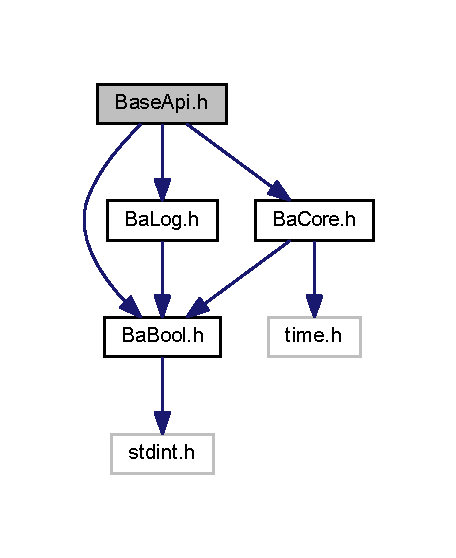
\includegraphics[width=219pt]{BaseApi_8h__incl}
\end{center}
\end{figure}
This graph shows which files directly or indirectly include this file\+:\nopagebreak
\begin{figure}[H]
\begin{center}
\leavevmode
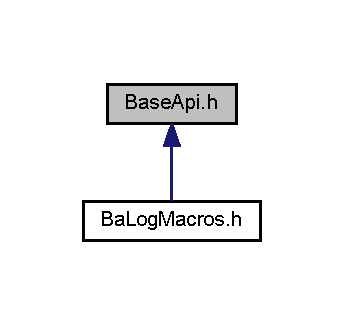
\includegraphics[width=165pt]{BaseApi_8h__dep__incl}
\end{center}
\end{figure}
\subsection*{Classes}
\begin{DoxyCompactItemize}
\item 
struct \hyperlink{structTBaApiCtrlTaskOpts}{T\+Ba\+Api\+Ctrl\+Task\+Opts}
\begin{DoxyCompactList}\small\item\em Options structure for the control task started with \hyperlink{BaseApi_8h_a60c99fae43923e540eaafa66bfe17508}{Ba\+Api\+Start\+Ctrl\+Task()} \end{DoxyCompactList}\item 
struct \hyperlink{structTBaApiCtrlTaskStats}{T\+Ba\+Api\+Ctrl\+Task\+Stats}
\begin{DoxyCompactList}\small\item\em Control task statistics. \end{DoxyCompactList}\end{DoxyCompactItemize}
\subsection*{Typedefs}
\begin{DoxyCompactItemize}
\item 
\hypertarget{BaseApi_8h_a948249cb0b015107c2cb5e88149b42cc}{}typedef struct \hyperlink{structTBaApiCtrlTaskOpts}{T\+Ba\+Api\+Ctrl\+Task\+Opts} \hyperlink{BaseApi_8h_a948249cb0b015107c2cb5e88149b42cc}{T\+Ba\+Api\+Ctrl\+Task\+Opts}\label{BaseApi_8h_a948249cb0b015107c2cb5e88149b42cc}

\begin{DoxyCompactList}\small\item\em Options structure for the control task started with \hyperlink{BaseApi_8h_a60c99fae43923e540eaafa66bfe17508}{Ba\+Api\+Start\+Ctrl\+Task()} \end{DoxyCompactList}\item 
\hypertarget{BaseApi_8h_ab5b91434be9ec71d18180600c490503b}{}typedef struct \hyperlink{structTBaApiCtrlTaskStats}{T\+Ba\+Api\+Ctrl\+Task\+Stats} \hyperlink{BaseApi_8h_ab5b91434be9ec71d18180600c490503b}{T\+Ba\+Api\+Ctrl\+Task\+Stats}\label{BaseApi_8h_ab5b91434be9ec71d18180600c490503b}

\begin{DoxyCompactList}\small\item\em Control task statistics. \end{DoxyCompactList}\end{DoxyCompactItemize}
\subsection*{Functions}
\begin{DoxyCompactItemize}
\item 
\hyperlink{BaBool_8h_a84d5a0de4729ca4c89f2479c605dbf3d}{T\+Ba\+Bool\+R\+C} \hyperlink{BaseApi_8h_a1914573ea9bce1d0ebe2c6ed0ac0ec2b}{Ba\+Api\+Log\+F} (\hyperlink{BaLog_8h_ab14f00a81932b8b62d2e8c4a2d7e3916}{E\+Ba\+Log\+Prio} prio, const char $\ast$tag, const char $\ast$fmt,...)
\begin{DoxyCompactList}\small\item\em Logging function that uses the the logger initialized with \hyperlink{BaseApi_8h_a67e6e46fba28f5337c7bfe6f8c15445d}{Ba\+Api\+Init\+Logger()} or \hyperlink{BaseApi_8h_a39fa5faacc955b4f2efb3fd0ea54be62}{Ba\+Api\+Init\+Logger\+Def()} \end{DoxyCompactList}\end{DoxyCompactItemize}
\begin{Indent}{\bf Resource Management}\par
\begin{DoxyCompactItemize}
\item 
\hyperlink{BaBool_8h_a84d5a0de4729ca4c89f2479c605dbf3d}{T\+Ba\+Bool\+R\+C} \hyperlink{BaseApi_8h_afd34d44879e18b4439f7758dc039e2e5}{Ba\+Api\+Init} ()
\begin{DoxyCompactList}\small\item\em todo\+: stub \end{DoxyCompactList}\item 
\hyperlink{BaBool_8h_a84d5a0de4729ca4c89f2479c605dbf3d}{T\+Ba\+Bool\+R\+C} \hyperlink{BaseApi_8h_a94ed4f951d7c8059ecc76fb973c027a3}{Ba\+Api\+Exit} ()
\begin{DoxyCompactList}\small\item\em todo\+: stub \end{DoxyCompactList}\item 
\hyperlink{BaBool_8h_a84d5a0de4729ca4c89f2479c605dbf3d}{T\+Ba\+Bool\+R\+C} \hyperlink{BaseApi_8h_a39fa5faacc955b4f2efb3fd0ea54be62}{Ba\+Api\+Init\+Logger\+Def} (const char $\ast$name)
\begin{DoxyCompactList}\small\item\em Initializes the logger that will be used throughout this A\+P\+I with default options. \end{DoxyCompactList}\item 
\hyperlink{BaBool_8h_a84d5a0de4729ca4c89f2479c605dbf3d}{T\+Ba\+Bool\+R\+C} \hyperlink{BaseApi_8h_a67e6e46fba28f5337c7bfe6f8c15445d}{Ba\+Api\+Init\+Logger} (T\+Ba\+Log\+Desc log)
\begin{DoxyCompactList}\small\item\em Initializes the logger that will be used throughout this A\+P\+I. \end{DoxyCompactList}\item 
\hyperlink{BaBool_8h_a84d5a0de4729ca4c89f2479c605dbf3d}{T\+Ba\+Bool\+R\+C} \hyperlink{BaseApi_8h_a8ec0422be53a6b3d78c1fbd310372711}{Ba\+Api\+Exit\+Logger} ()
\begin{DoxyCompactList}\small\item\em Releases the resources of the general logger. \end{DoxyCompactList}\end{DoxyCompactItemize}
\end{Indent}
\begin{Indent}{\bf Control Task}\par
\begin{DoxyCompactItemize}
\item 
\hyperlink{BaBool_8h_a84d5a0de4729ca4c89f2479c605dbf3d}{T\+Ba\+Bool\+R\+C} \hyperlink{BaseApi_8h_a60c99fae43923e540eaafa66bfe17508}{Ba\+Api\+Start\+Ctrl\+Task} (const \hyperlink{structTBaApiCtrlTaskOpts}{T\+Ba\+Api\+Ctrl\+Task\+Opts} $\ast$p\+Opts)
\begin{DoxyCompactList}\small\item\em Starts the one and only control task as a new process. \end{DoxyCompactList}\item 
\hyperlink{BaBool_8h_a84d5a0de4729ca4c89f2479c605dbf3d}{T\+Ba\+Bool\+R\+C} \hyperlink{BaseApi_8h_a55d72c35323e5ffaa7219d7fb54f4bf1}{Ba\+Api\+Stop\+Ctrl\+Task} ()
\begin{DoxyCompactList}\small\item\em Stops the one and only control task. \end{DoxyCompactList}\item 
\hyperlink{BaBool_8h_a84d5a0de4729ca4c89f2479c605dbf3d}{T\+Ba\+Bool\+R\+C} \hyperlink{BaseApi_8h_a81ad517fcd3fbf12c5fc57273eb0ce94}{Ba\+Api\+Start\+Ctrl\+Thread} (const \hyperlink{structTBaApiCtrlTaskOpts}{T\+Ba\+Api\+Ctrl\+Task\+Opts} $\ast$p\+Opts)
\begin{DoxyCompactList}\small\item\em Starts the one and only control thread as a new thread. \end{DoxyCompactList}\item 
\hyperlink{BaBool_8h_a84d5a0de4729ca4c89f2479c605dbf3d}{T\+Ba\+Bool\+R\+C} \hyperlink{BaseApi_8h_abf560df382cc0fa41c71a555a567befd}{Ba\+Api\+Stop\+Ctrl\+Thread} ()
\begin{DoxyCompactList}\small\item\em Stops the one and only control thread. \end{DoxyCompactList}\item 
\hyperlink{BaBool_8h_a84d5a0de4729ca4c89f2479c605dbf3d}{T\+Ba\+Bool\+R\+C} \hyperlink{BaseApi_8h_a2a738f0b607a8c4fb3b2bcfd0e4f5bcc}{Ba\+Api\+Get\+Ctrl\+Task\+Stats} (\hyperlink{structTBaApiCtrlTaskStats}{T\+Ba\+Api\+Ctrl\+Task\+Stats} $\ast$p\+Stats)
\begin{DoxyCompactList}\small\item\em Gets the task statistics. \end{DoxyCompactList}\end{DoxyCompactItemize}
\end{Indent}


\subsection{Detailed Description}
Includes the following\+: 


\begin{DoxyItemize}
\item A\+P\+I wide logger
\item Control task 
\end{DoxyItemize}

\subsection{Function Documentation}
\hypertarget{BaseApi_8h_afd34d44879e18b4439f7758dc039e2e5}{}\index{Base\+Api.\+h@{Base\+Api.\+h}!Ba\+Api\+Init@{Ba\+Api\+Init}}
\index{Ba\+Api\+Init@{Ba\+Api\+Init}!Base\+Api.\+h@{Base\+Api.\+h}}
\subsubsection[{Ba\+Api\+Init()}]{\setlength{\rightskip}{0pt plus 5cm}{\bf T\+Ba\+Bool\+R\+C} Ba\+Api\+Init (
\begin{DoxyParamCaption}
{}
\end{DoxyParamCaption}
)}\label{BaseApi_8h_afd34d44879e18b4439f7758dc039e2e5}


todo\+: stub 

\begin{DoxyReturn}{Returns}
Error or success 
\end{DoxyReturn}
\hypertarget{BaseApi_8h_a94ed4f951d7c8059ecc76fb973c027a3}{}\index{Base\+Api.\+h@{Base\+Api.\+h}!Ba\+Api\+Exit@{Ba\+Api\+Exit}}
\index{Ba\+Api\+Exit@{Ba\+Api\+Exit}!Base\+Api.\+h@{Base\+Api.\+h}}
\subsubsection[{Ba\+Api\+Exit()}]{\setlength{\rightskip}{0pt plus 5cm}{\bf T\+Ba\+Bool\+R\+C} Ba\+Api\+Exit (
\begin{DoxyParamCaption}
{}
\end{DoxyParamCaption}
)}\label{BaseApi_8h_a94ed4f951d7c8059ecc76fb973c027a3}


todo\+: stub 

\begin{DoxyReturn}{Returns}
Error or success 
\end{DoxyReturn}
\hypertarget{BaseApi_8h_a39fa5faacc955b4f2efb3fd0ea54be62}{}\index{Base\+Api.\+h@{Base\+Api.\+h}!Ba\+Api\+Init\+Logger\+Def@{Ba\+Api\+Init\+Logger\+Def}}
\index{Ba\+Api\+Init\+Logger\+Def@{Ba\+Api\+Init\+Logger\+Def}!Base\+Api.\+h@{Base\+Api.\+h}}
\subsubsection[{Ba\+Api\+Init\+Logger\+Def(const char $\ast$name)}]{\setlength{\rightskip}{0pt plus 5cm}{\bf T\+Ba\+Bool\+R\+C} Ba\+Api\+Init\+Logger\+Def (
\begin{DoxyParamCaption}
\item[{const char $\ast$}]{name}
\end{DoxyParamCaption}
)}\label{BaseApi_8h_a39fa5faacc955b4f2efb3fd0ea54be62}


Initializes the logger that will be used throughout this A\+P\+I with default options. 

\begin{DoxyReturn}{Returns}
Error or success 
\end{DoxyReturn}

\begin{DoxyParams}[1]{Parameters}
\mbox{\tt in}  & {\em name} & Name of the default logger \\
\hline
\end{DoxyParams}
\hypertarget{BaseApi_8h_a67e6e46fba28f5337c7bfe6f8c15445d}{}\index{Base\+Api.\+h@{Base\+Api.\+h}!Ba\+Api\+Init\+Logger@{Ba\+Api\+Init\+Logger}}
\index{Ba\+Api\+Init\+Logger@{Ba\+Api\+Init\+Logger}!Base\+Api.\+h@{Base\+Api.\+h}}
\subsubsection[{Ba\+Api\+Init\+Logger(\+T\+Ba\+Log\+Desc log)}]{\setlength{\rightskip}{0pt plus 5cm}{\bf T\+Ba\+Bool\+R\+C} Ba\+Api\+Init\+Logger (
\begin{DoxyParamCaption}
\item[{T\+Ba\+Log\+Desc}]{log}
\end{DoxyParamCaption}
)}\label{BaseApi_8h_a67e6e46fba28f5337c7bfe6f8c15445d}


Initializes the logger that will be used throughout this A\+P\+I. 

\begin{DoxyReturn}{Returns}
Error or success 
\end{DoxyReturn}

\begin{DoxyParams}[1]{Parameters}
\mbox{\tt in}  & {\em log} & Logger handle \\
\hline
\end{DoxyParams}
\hypertarget{BaseApi_8h_a8ec0422be53a6b3d78c1fbd310372711}{}\index{Base\+Api.\+h@{Base\+Api.\+h}!Ba\+Api\+Exit\+Logger@{Ba\+Api\+Exit\+Logger}}
\index{Ba\+Api\+Exit\+Logger@{Ba\+Api\+Exit\+Logger}!Base\+Api.\+h@{Base\+Api.\+h}}
\subsubsection[{Ba\+Api\+Exit\+Logger()}]{\setlength{\rightskip}{0pt plus 5cm}{\bf T\+Ba\+Bool\+R\+C} Ba\+Api\+Exit\+Logger (
\begin{DoxyParamCaption}
{}
\end{DoxyParamCaption}
)}\label{BaseApi_8h_a8ec0422be53a6b3d78c1fbd310372711}


Releases the resources of the general logger. 

\begin{DoxyReturn}{Returns}
Error or success 
\end{DoxyReturn}
\hypertarget{BaseApi_8h_a1914573ea9bce1d0ebe2c6ed0ac0ec2b}{}\index{Base\+Api.\+h@{Base\+Api.\+h}!Ba\+Api\+Log\+F@{Ba\+Api\+Log\+F}}
\index{Ba\+Api\+Log\+F@{Ba\+Api\+Log\+F}!Base\+Api.\+h@{Base\+Api.\+h}}
\subsubsection[{Ba\+Api\+Log\+F(\+E\+Ba\+Log\+Prio prio, const char $\ast$tag, const char $\ast$fmt,...)}]{\setlength{\rightskip}{0pt plus 5cm}{\bf T\+Ba\+Bool\+R\+C} Ba\+Api\+Log\+F (
\begin{DoxyParamCaption}
\item[{{\bf E\+Ba\+Log\+Prio}}]{prio, }
\item[{const char $\ast$}]{tag, }
\item[{const char $\ast$}]{fmt, }
\item[{}]{...}
\end{DoxyParamCaption}
)}\label{BaseApi_8h_a1914573ea9bce1d0ebe2c6ed0ac0ec2b}


Logging function that uses the the logger initialized with \hyperlink{BaseApi_8h_a67e6e46fba28f5337c7bfe6f8c15445d}{Ba\+Api\+Init\+Logger()} or \hyperlink{BaseApi_8h_a39fa5faacc955b4f2efb3fd0ea54be62}{Ba\+Api\+Init\+Logger\+Def()} 

\begin{DoxyReturn}{Returns}
Error or success 
\end{DoxyReturn}

\begin{DoxyParams}[1]{Parameters}
\mbox{\tt in}  & {\em prio} & Priority \\
\hline
\mbox{\tt in}  & {\em tag} & Tag to track or group the message \\
\hline
\mbox{\tt in}  & {\em fmt} & The message format \\
\hline
\end{DoxyParams}
\hypertarget{BaseApi_8h_a60c99fae43923e540eaafa66bfe17508}{}\index{Base\+Api.\+h@{Base\+Api.\+h}!Ba\+Api\+Start\+Ctrl\+Task@{Ba\+Api\+Start\+Ctrl\+Task}}
\index{Ba\+Api\+Start\+Ctrl\+Task@{Ba\+Api\+Start\+Ctrl\+Task}!Base\+Api.\+h@{Base\+Api.\+h}}
\subsubsection[{Ba\+Api\+Start\+Ctrl\+Task(const T\+Ba\+Api\+Ctrl\+Task\+Opts $\ast$p\+Opts)}]{\setlength{\rightskip}{0pt plus 5cm}{\bf T\+Ba\+Bool\+R\+C} Ba\+Api\+Start\+Ctrl\+Task (
\begin{DoxyParamCaption}
\item[{const {\bf T\+Ba\+Api\+Ctrl\+Task\+Opts} $\ast$}]{p\+Opts}
\end{DoxyParamCaption}
)}\label{BaseApi_8h_a60c99fae43923e540eaafa66bfe17508}


Starts the one and only control task as a new process. 

This also automatically initializes the default logger if it not previously initialized via \hyperlink{BaseApi_8h_a67e6e46fba28f5337c7bfe6f8c15445d}{Ba\+Api\+Init\+Logger()}. If a specialized logger is required, one could initialize it in the init() callback \begin{DoxyReturn}{Returns}
Error or success 
\end{DoxyReturn}

\begin{DoxyParams}[1]{Parameters}
\mbox{\tt in}  & {\em p\+Opts} & Task options \\
\hline
\end{DoxyParams}
\hypertarget{BaseApi_8h_a55d72c35323e5ffaa7219d7fb54f4bf1}{}\index{Base\+Api.\+h@{Base\+Api.\+h}!Ba\+Api\+Stop\+Ctrl\+Task@{Ba\+Api\+Stop\+Ctrl\+Task}}
\index{Ba\+Api\+Stop\+Ctrl\+Task@{Ba\+Api\+Stop\+Ctrl\+Task}!Base\+Api.\+h@{Base\+Api.\+h}}
\subsubsection[{Ba\+Api\+Stop\+Ctrl\+Task()}]{\setlength{\rightskip}{0pt plus 5cm}{\bf T\+Ba\+Bool\+R\+C} Ba\+Api\+Stop\+Ctrl\+Task (
\begin{DoxyParamCaption}
{}
\end{DoxyParamCaption}
)}\label{BaseApi_8h_a55d72c35323e5ffaa7219d7fb54f4bf1}


Stops the one and only control task. 

\begin{DoxyReturn}{Returns}
Error or success 
\end{DoxyReturn}
\hypertarget{BaseApi_8h_a81ad517fcd3fbf12c5fc57273eb0ce94}{}\index{Base\+Api.\+h@{Base\+Api.\+h}!Ba\+Api\+Start\+Ctrl\+Thread@{Ba\+Api\+Start\+Ctrl\+Thread}}
\index{Ba\+Api\+Start\+Ctrl\+Thread@{Ba\+Api\+Start\+Ctrl\+Thread}!Base\+Api.\+h@{Base\+Api.\+h}}
\subsubsection[{Ba\+Api\+Start\+Ctrl\+Thread(const T\+Ba\+Api\+Ctrl\+Task\+Opts $\ast$p\+Opts)}]{\setlength{\rightskip}{0pt plus 5cm}{\bf T\+Ba\+Bool\+R\+C} Ba\+Api\+Start\+Ctrl\+Thread (
\begin{DoxyParamCaption}
\item[{const {\bf T\+Ba\+Api\+Ctrl\+Task\+Opts} $\ast$}]{p\+Opts}
\end{DoxyParamCaption}
)}\label{BaseApi_8h_a81ad517fcd3fbf12c5fc57273eb0ce94}


Starts the one and only control thread as a new thread. 

This is mainly for debugging and development. For proper releases use \hyperlink{BaseApi_8h_a60c99fae43923e540eaafa66bfe17508}{Ba\+Api\+Start\+Ctrl\+Task()}. \begin{DoxyReturn}{Returns}
Error or success 
\end{DoxyReturn}

\begin{DoxyParams}[1]{Parameters}
\mbox{\tt in}  & {\em p\+Opts} & Task options \\
\hline
\end{DoxyParams}
\hypertarget{BaseApi_8h_abf560df382cc0fa41c71a555a567befd}{}\index{Base\+Api.\+h@{Base\+Api.\+h}!Ba\+Api\+Stop\+Ctrl\+Thread@{Ba\+Api\+Stop\+Ctrl\+Thread}}
\index{Ba\+Api\+Stop\+Ctrl\+Thread@{Ba\+Api\+Stop\+Ctrl\+Thread}!Base\+Api.\+h@{Base\+Api.\+h}}
\subsubsection[{Ba\+Api\+Stop\+Ctrl\+Thread()}]{\setlength{\rightskip}{0pt plus 5cm}{\bf T\+Ba\+Bool\+R\+C} Ba\+Api\+Stop\+Ctrl\+Thread (
\begin{DoxyParamCaption}
{}
\end{DoxyParamCaption}
)}\label{BaseApi_8h_abf560df382cc0fa41c71a555a567befd}


Stops the one and only control thread. 

\begin{DoxyReturn}{Returns}
Error or success 
\end{DoxyReturn}
\hypertarget{BaseApi_8h_a2a738f0b607a8c4fb3b2bcfd0e4f5bcc}{}\index{Base\+Api.\+h@{Base\+Api.\+h}!Ba\+Api\+Get\+Ctrl\+Task\+Stats@{Ba\+Api\+Get\+Ctrl\+Task\+Stats}}
\index{Ba\+Api\+Get\+Ctrl\+Task\+Stats@{Ba\+Api\+Get\+Ctrl\+Task\+Stats}!Base\+Api.\+h@{Base\+Api.\+h}}
\subsubsection[{Ba\+Api\+Get\+Ctrl\+Task\+Stats(\+T\+Ba\+Api\+Ctrl\+Task\+Stats $\ast$p\+Stats)}]{\setlength{\rightskip}{0pt plus 5cm}{\bf T\+Ba\+Bool\+R\+C} Ba\+Api\+Get\+Ctrl\+Task\+Stats (
\begin{DoxyParamCaption}
\item[{{\bf T\+Ba\+Api\+Ctrl\+Task\+Stats} $\ast$}]{p\+Stats}
\end{DoxyParamCaption}
)}\label{BaseApi_8h_a2a738f0b607a8c4fb3b2bcfd0e4f5bcc}


Gets the task statistics. 

This is mostly meant to be called within the {\ttfamily update()} function so it gets the statistics from the control task \begin{DoxyReturn}{Returns}
Error or success 
\end{DoxyReturn}

\begin{DoxyParams}[1]{Parameters}
\mbox{\tt out}  & {\em p\+Stats} & Statistics \\
\hline
\end{DoxyParams}

\hypertarget{BaUtils_8hpp}{}\section{Ba\+Utils.\+hpp File Reference}
\label{BaUtils_8hpp}\index{Ba\+Utils.\+hpp@{Ba\+Utils.\+hpp}}


General useful functions.  


{\ttfamily \#include $<$string$>$}\\*
{\ttfamily \#include $<$istream$>$}\\*
Include dependency graph for Ba\+Utils.\+hpp\+:\nopagebreak
\begin{figure}[H]
\begin{center}
\leavevmode
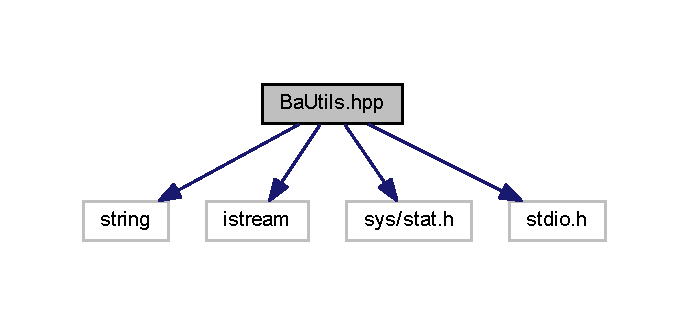
\includegraphics[width=188pt]{BaUtils_8hpp__incl}
\end{center}
\end{figure}


\subsection{Detailed Description}
General useful functions. 


%--- End generated contents ---

% Index
\backmatter
\newpage
\phantomsection
\clearemptydoublepage
\addcontentsline{toc}{chapter}{Index}
\printindex

\end{document}
